\documentclass[a4paper, 12pt, oneside]{memoir}


\usepackage[utf8]{inputenc}
\usepackage[T1]{fontenc}
\usepackage{charter}
% \usepackage[bitstream-charter]{mathdesign}
\usepackage[francais,english]{babel}
\usepackage[x11names, rgb]{xcolor}
\usepackage{geometry}
\usepackage[pdftex]{graphicx}
\usepackage{tikz}
\usepackage{pgfplots}%Needed at least by {axis} environment
\pgfplotsset{compat = 1.3}%1.3 needed by 'ylabel shift = 1 em'

\usepackage{graphicx}
\usepackage{listings}
\usepackage{picture}
\usepackage{epic}
\usepackage{verbatim}
\usepackage{textcomp}
\usepackage{tabularx}
\usepackage{multirow}
\usepackage{array}
% \usepackage[breaklinks=true,hidelinks]{hyperref}
\usepackage{memhfixc}
\usepackage[breaklinks=true]{hyperref}

\usepackage[numbers]{natbib}

\usepackage{framed}
\usepackage{listings}
\definecolor{colKeys}{rgb}{0,0,1}  % couleurs des mots-clés propres au language
\definecolor{colIdentifier}{rgb}{0,0,0}  % couleurs des mots à identifier
\definecolor{colComments}{rgb}{0,0.6,0}  % couleurs des commentaires
\definecolor{colString}{rgb}{0.6,0.1,0.1}

\setcounter{secnumdepth}{3}% Number up to subsubsection
\maxsecnumdepth{subsubsection}% 'secnumdepth' is reset by \mainmatter. You should use 'maxsecnumdepth'.
% \seccounter{tocdepth}{3}% Add subsubsection to the table of content.



% ----------------------
% Cover page
% ----------------------

% Logos
\newcommand{\ulb}{
\includegraphics[scale=1.1]{logo_ULB2.pdf}}
\newcommand{\polytech}{
\includegraphics[scale=0.35]{logo_polytech_FR.pdf}}

% Polices
\definecolor{ULBblue}{rgb}{0,0.2196,0.5765}
\newcommand{\fontTitle}{\sffamily \Huge\selectfont \color{ULBblue}}
\newcommand{\fontSubtitle}{\sffamily \LARGE \selectfont \color{ULBblue}}
\newcommand{\fontText}{\sffamily \selectfont}
\newcommand{\fontColor}{\sffamily \selectfont \color{ULBblue}}

% Titre
\newcommand{\titleA}{\fontTitle{Implementation of High-Level Cryptographic}} % Titre identique au titre remis au secrétariat
\newcommand{\titleB}{\fontTitle{Protocols using a SoC Platform}} % (dans la langue de rédaction a priori)
% Sous-titre
%\newcommand{\subtitle}{\fontSubtitle{Ligne du sous-titre du mémoire}}
% Titre du diplôme
\newcommand{\diplomaA}{\fontText{Mémoire présenté en vue de l’obtention du diplôme}} % A laisser en Français
\newcommand{\diplomaB}{\fontText{d'Ingénieur Civil en informatique à finalité spécialisée}}

% Etudiant
\newcommand{\student}{\textbf{\sffamily \large Quentin Delhaye}}

% Supervision
\newcommand{\promAa}{\fontColor{Directeur}}
\newcommand{\promAb}{\fontText{Professeur Frédéric Robert}}
% \newcommand{\promBa}{\fontColor{Co-Promoteur}}
% \newcommand{\promBb}{\fontText{Professeur [Prénom Nom]}}
\newcommand{\promCa}{\fontColor{Superviseur}}
\newcommand{\promCb}{\fontText{Sébastien Rabou (Barco Silex)}}
\newcommand{\deptA}{\fontColor{Service}}
\newcommand{\deptB}{\fontText{BEAMS}}

% Année académique
\newcommand{\yearA}{\fontColor{Année académique}}
\newcommand{\yearB}{\fontText{2014 - 2015}}

\begin{document}

\frontmatter

\documentclass[a4paper, 12pt]{report}

\usepackage[utf8]{inputenc}
\usepackage{color}
\usepackage[top=2.5cm, bottom=1.5cm, left=2.5cm, right=1cm]{geometry}
\usepackage[pdftex]{graphicx}
\usepackage{tikz}

% Logos
\newcommand{\ulb}{
\includegraphics[scale=1.1]{logo_ULB2.pdf}}
\newcommand{\polytech}{
\includegraphics[scale=0.35]{logo_polytech_FR.pdf}}

% Polices
\definecolor{ULBblue}{rgb}{0,0.2196,0.5765}
\newcommand{\fontTitle}{\sffamily \Huge\selectfont \color{ULBblue}}
\newcommand{\fontSubtitle}{\sffamily \LARGE \selectfont \color{ULBblue}}
\newcommand{\fontText}{\sffamily \selectfont}
\newcommand{\fontColor}{\sffamily \selectfont \color{ULBblue}}

% Titre
\newcommand{\titleA}{\fontTitle{Implementation of High-Level Cryptographic}} % Titre identique au titre remis au secrétariat
\newcommand{\titleB}{\fontTitle{Protocols using a SoC Plateform}} % (dans la langue de rédaction a priori)
% Sous-titre
%\newcommand{\subtitle}{\fontSubtitle{Ligne du sous-titre du mémoire}}
% Titre du diplôme
\newcommand{\diplomaA}{\fontText{Mémoire présenté en vue de l’obtention du diplôme}} % A laisser en Français
\newcommand{\diplomaB}{\fontText{d'Ingénieur Civil en informatique à finalité spécialisée}}

% Etudiant
\newcommand{\student}{\textbf{\sffamily \large Quentin Delhaye}}

% Supervision
\newcommand{\promAa}{\fontColor{Directeur}}
\newcommand{\promAb}{\fontText{Professeur Frédéric Robert}}
% \newcommand{\promBa}{\fontColor{Co-Promoteur}}
% \newcommand{\promBb}{\fontText{Professeur [Prénom Nom]}}
\newcommand{\promCa}{\fontColor{Superviseur}}
\newcommand{\promCb}{\fontText{Sébastien Rabou (Barco Silex)}}
\newcommand{\deptA}{\fontColor{Service}}
\newcommand{\deptB}{\fontText{BEAMS}}

% Année académique
\newcommand{\yearA}{\fontColor{Année académique}}
\newcommand{\yearB}{\fontText{2014 - 2015}}

\begin{document}

	\thispagestyle{empty}
	\newgeometry{top=2.5cm, bottom=1.5cm, left=2.5cm, right=1cm}
	\setlength{\unitlength}{1mm}
	\noindent\begin{picture}(175,257)
	
		\put(0,245){\polytech}
		\put(153,139.5){\ulb}
		
		\put(8,155){\makebox(150,10)[l]{\titleA}}
		\put(8,145){\makebox(150,10)[l]{\titleB}}
		% \put(8,135){\makebox(150,10)[l]{\subtitle}}
		
		\put(0,75){
		\begin{tikzpicture}[scale=0.1]
		\fill [fill=ULBblue](0,0) rectangle (0.8,90);
		\fill [fill=ULBblue](0,57) rectangle (152,57.8);
		\end{tikzpicture}}
		
		\put(8,120){\makebox(150,5)[l]{\diplomaA}}
		\put(8,115){\makebox(150,5)[l]{\diplomaB}}
		
		\put(8,75){\makebox(150,10)[l]{\selectfont \student}}
		
		% \put(8,44){\makebox(80,5)[l]{\promAa}}
		% \put(8,39){\makebox(80,5)[l]{\promAb}}
		\put(8,31){\makebox(80,5)[l]{\promAa}}
		\put(8,26){\makebox(80,5)[l]{\promAb}}
		% \put(8,31){\makebox(80,5)[l]{\promBa}} % Commenter la ligne si pas nécessaire
		% \put(8,26){\makebox(80,5)[l]{\promBb}} % Commenter la ligne si pas nécessaire
		\put(8,18){\makebox(80,5)[l]{\promCa}} % Commenter la ligne si pas nécessaire
		\put(8,13){\makebox(80,5)[l]{\promCb}} % Commenter la ligne si pas nécessaire
		\put(8,5){\makebox(80,5)[l]{\deptA}}
		\put(8,0){\makebox(80,5)[l]{\deptB}}
		
		\put(145,5){\makebox(30,5)[r]{\yearA}}
		\put(145,0){\makebox(30,5)[r]{\yearB}}
	
	\end{picture}
	\restoregeometry

\end{document}

% Template conçu par Benjamin Vanhemelryck et revu par François Bronchart - Mai 2013
\setcounter{page}{1}
\newgeometry{bottom=2.5cm}

\addcontentsline{toc}{chapter}{\numberline{}Aknowledgements}
\chapter*{Aknowledgements}

\thispagestyle{plain}% This way, we can have the page numbering in the foot.
\selectlanguage{english}
% \renewcommand{\abstractname}{\Large{The \lego Motorcyclist robot}}
\addcontentsline{toc}{chapter}{\numberline{}Abstract}
\begin{abstract}
	\begin{verse}
	\small \textit{
	by Quentin Delhaye, Arnaud Dumont, Camille Giaux, Pierre Lasbleis and  Gauthier Roig; Université Libre de Bruxelles, 2011–2012.}
	\normalsize
	\end{verse}
\end{abstract}

\clearpage

\thispagestyle{plain}
\selectlanguage{francais}
% \renewcommand{\abstractname}{\Large{Le robot motard \lego}}
\addcontentsline{toc}{chapter}{\numberline{}Résumé}
\begin{abstract}
	\begin{verse}
	\small \textit{
	par Quentin Delhaye, Arnaud Dumont, Camille Giaux, Pierre Lasbleis et Gauthier Roig ; Université Libre de Bruxelles, 2011–2012.}
	\normalsize
	\end{verse}
\end{abstract}

\selectlanguage{english}
\tableofcontents \pagebreak
\listoffigures \pagebreak

\mainmatter

\chapter{Introduction}
% What is hardware offloading?

Altera and Xilinx are trying to push those SoC plateforms to the market to popularize the FPGAs.

Power is critical nowadays, esapcially in datacenters.
Several solutions exists: abandonning general purpose processors altoghether and turn towards ARM cores, or add an FPGA to the processor for example.
Intel proposed the latter solution in 2014~\cite{intel-xeon-fpga} and is on its way to expand that market with the merger with Altera~\cite{intel-altera-merger}.

There a re diffirent ways to add cryptographic capabilities to an application:
\begin{itemize}
	\item Having the cipher built in.
	\item Using a cryptographic library, such as OpenSSL.
	\item Using the Linux Crypto API.
\end{itemize}

Present the two IP cores that will be used in this work: BA411E and BA414E.


\section{Challenge}

\section{Network security}%=> What is the problematic of the thesis? What is the challenge? What do we want to show?

\chapter{Technical background}\label{chap:theory}

This chapter will address the technical ground necessary to this work.
First comes a quick presentation of FPGAs and how they can be driven from the operating system.

\noindent Follows an overview of Linux operating systems, the distinction between user and kernel mode, and the design of device drivers.

\noindent Next comes an overview of the cryptographic field with the main primitives: message digests, symmetric ciphers and asymmetric ciphers.

\noindent Finally, the ground necessary to understand the inner working and challenges of some VPNs implementations using SSL/TLS and IPsec will be covered.



%%%%%%%%%%%%%%%%%%%%%%%%%%%%%%%%%%%%%%%%%%%%%%%%%%%%%%%%%%%%%%%%%%%%%%%%%%%%%%%%
\section{FPGA}
%%%%%%%%%%%%%%%%%%%%%%%%%%%%%%%%%%%%%%%%%%%%%%%%%%%%%%%%%%%%%%%%%%%%%%%%%%%%%%%%
The aim of this work is to study the impact of offloading cryptographic operations in hardware.
In order to reach that goal, an FPGA will be used.

A Field-Prgrammable Gate Array (FPGA) is an integrated circuit that can be programmed after the manufacturing, using a semiconductor intellectual property core (IP core).
In this work, we will use some of Barco Silex's crypto IP cores.

In order for the operating system to comunicate with the device, they will need to share some memory.
That memory can be directly mapped and accessed from the user-space using \texttt{/dev/mem}, or can use a direct memory access module (DMA).
From the operating system, we build a bunch of scatterlist in the kernel-space memory, then map those pages to memory descriptor that have a physical address on the DMA.
They can be mapped three different ways: \texttt{DMA\_BIDIRECTIONAL}, \texttt{DMA\_TO\_DEVICE} or \texttt{DMA\_FROM\_DEVICE}.
When the CPU write something in those descriptors and synchronize them with the DMA, it does not have to care about them anymore, the DMA in now in charge to send them to the device where registers are ready to read the incomming data.
The same goes from the device to the CPU: when the device wants to communicate data to the OS, it writes it on the DMA that will transfer them to the CPU, triggering a flag on the way to notify it.

\begin{figure}
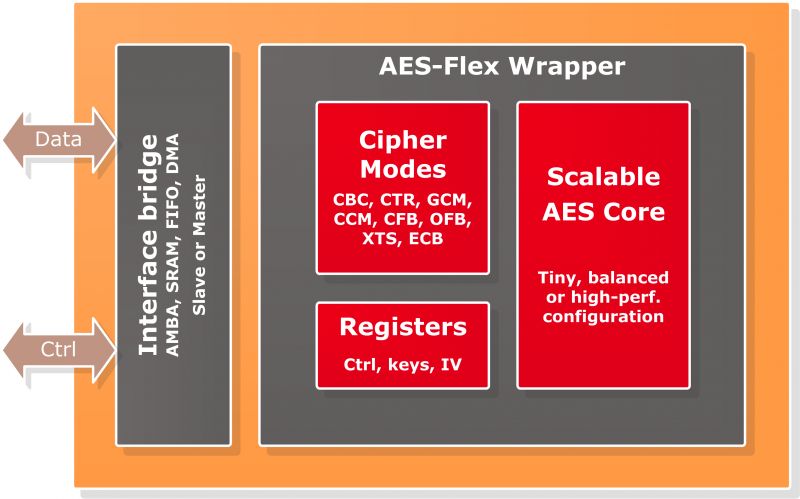
\includegraphics[width=\linewidth]{barco-ba411e-ipcore}
\caption{Barco Silex' AES IP Core}{There are two channels to comunicate with the IP core: the data and control paths~\cite{barco-ba411e}.}
\label{fig:barco-ba411e-ipcore}
\end{figure}

There are two types of interface with such a device: master or slave.
The figure~\ref{fig:barco-ba411e-ipcore}  represent one of Barco Silex' crypto IP cores that proposes two interfaces: one of each type.
\begin{itemize}
	\item The data path is a master. That is the operating system will not have a direct access to the memory registers of the hardware devide. Instead, they will communicate via a DMA bus: one peer places data on the DMA and notifies the other that he can fetch it.
	\item The control (ctrl) path is a slave. The operatin system can directly read and write on this part of the device memory.
\end{itemize}

A master interface has the advantage to offload a part of the memory management to the device, but there is a space overhead to connect the DMA as well as an extra delay to process its data.
A slave interface is usually used for sporadic data, avoiding the overhead of a DMA.
As an example, the data path of Barco Silex' symmetric cryptography IP core is a master, as there is a lot of data to process, whilst the same data path of their asymmetric cryptography IP core is a slave, for the operands are larger and the computation takes more time.



%%%%%%%%%%%%%%%%%%%%%%%%%%%%%%%%%%%%%%%%%%%%%%%%%%%%%%%%%%%%%%%%%%%%%%%%%%%%%%%%
\section{Operating system}
%%%%%%%%%%%%%%%%%%%%%%%%%%%%%%%%%%%%%%%%%%%%%%%%%%%%%%%%%%%%%%%%%%%%%%%%%%%%%%%%

%User/kernel space. Networking application: need to send the data through the kernel: huge overhead.

%Crypto API

Modern operating systems run on several levels of privilege.
Under Unix, the kernel runs under the highest level and it has no restriction, whereas applications run on the lowest level.
We call those two levels kernel space and user space, segragating the privilege and the memory between the two modes (\citet{tanenbaum2014} and \citet[chap. 2]{Corbet:2005:LDD:1209083}).
The figure~\ref{fig:user-kernel} shows this separation.
In order for the applications in the user space to reach the hardware, they need to go through the kernel and use the device drivers that are registered there.

\begin{figure}[ht]
\center
% Graphic for TeX using PGF
% Title: /home/para/documents/polytech2015/MA2/Master_thesis/master_thesis/user-kernel.dia
% Creator: Dia v0.97.3
% CreationDate: Thu May 28 03:32:07 2015
% For: para
% \usepackage{tikz}
% The following commands are not supported in PSTricks at present
% We define them conditionally, so when they are implemented,
% this pgf file will use them.
\ifx\du\undefined
  \newlength{\du}
\fi
\setlength{\du}{15\unitlength}
\begin{tikzpicture}
\pgftransformxscale{1.000000}
\pgftransformyscale{-1.000000}
\definecolor{dialinecolor}{rgb}{0.000000, 0.000000, 0.000000}
\pgfsetstrokecolor{dialinecolor}
\definecolor{dialinecolor}{rgb}{1.000000, 1.000000, 1.000000}
\pgfsetfillcolor{dialinecolor}
\pgfsetlinewidth{0.050000\du}
\pgfsetdash{}{0pt}
\pgfsetdash{}{0pt}
\pgfsetmiterjoin
\definecolor{dialinecolor}{rgb}{1.000000, 1.000000, 1.000000}
\pgfsetfillcolor{dialinecolor}
\fill (11.500000\du,7.400000\du)--(11.500000\du,9.200000\du)--(13.000000\du,9.200000\du)--(13.000000\du,7.400000\du)--cycle;
\definecolor{dialinecolor}{rgb}{0.000000, 0.000000, 0.000000}
\pgfsetstrokecolor{dialinecolor}
\draw (11.500000\du,7.400000\du)--(11.500000\du,9.200000\du)--(13.000000\du,9.200000\du)--(13.000000\du,7.400000\du)--cycle;
\pgfsetlinewidth{0.050000\du}
\pgfsetdash{}{0pt}
\pgfsetdash{}{0pt}
\pgfsetmiterjoin
\definecolor{dialinecolor}{rgb}{1.000000, 1.000000, 1.000000}
\pgfsetfillcolor{dialinecolor}
\fill (11.500000\du,7.400000\du)--(11.500000\du,9.400000\du)--(17.700000\du,9.400000\du)--(17.700000\du,7.400000\du)--cycle;
\definecolor{dialinecolor}{rgb}{0.000000, 0.000000, 0.000000}
\pgfsetstrokecolor{dialinecolor}
\draw (11.500000\du,7.400000\du)--(11.500000\du,9.400000\du)--(17.700000\du,9.400000\du)--(17.700000\du,7.400000\du)--cycle;
% setfont left to latex
\definecolor{dialinecolor}{rgb}{0.000000, 0.000000, 0.000000}
\pgfsetstrokecolor{dialinecolor}
\node at (12.250000\du,8.300000\du){User};
\pgfsetlinewidth{0.050000\du}
\pgfsetdash{}{0pt}
\pgfsetdash{}{0pt}
\pgfsetmiterjoin
\definecolor{dialinecolor}{rgb}{1.000000, 1.000000, 1.000000}
\pgfsetfillcolor{dialinecolor}
\fill (11.500000\du,9.600000\du)--(11.500000\du,12.700000\du)--(13.000000\du,12.700000\du)--(13.000000\du,9.600000\du)--cycle;
\definecolor{dialinecolor}{rgb}{0.000000, 0.000000, 0.000000}
\pgfsetstrokecolor{dialinecolor}
\draw (11.500000\du,9.600000\du)--(11.500000\du,12.700000\du)--(13.000000\du,12.700000\du)--(13.000000\du,9.600000\du)--cycle;
\pgfsetlinewidth{0.050000\du}
\pgfsetdash{}{0pt}
\pgfsetdash{}{0pt}
\pgfsetmiterjoin
\definecolor{dialinecolor}{rgb}{0.905882, 0.905882, 0.905882}
\pgfsetfillcolor{dialinecolor}
\fill (11.500000\du,9.600000\du)--(11.500000\du,12.700000\du)--(17.700000\du,12.700000\du)--(17.700000\du,9.600000\du)--cycle;
\definecolor{dialinecolor}{rgb}{0.000000, 0.000000, 0.000000}
\pgfsetstrokecolor{dialinecolor}
\draw (11.500000\du,9.600000\du)--(11.500000\du,12.700000\du)--(17.700000\du,12.700000\du)--(17.700000\du,9.600000\du)--cycle;
% setfont left to latex
\definecolor{dialinecolor}{rgb}{0.000000, 0.000000, 0.000000}
\pgfsetstrokecolor{dialinecolor}
\node at (12.250000\du,11.150000\du){Kernel};
\pgfsetlinewidth{0.050000\du}
\pgfsetdash{}{0pt}
\pgfsetdash{}{0pt}
\pgfsetmiterjoin
\definecolor{dialinecolor}{rgb}{1.000000, 1.000000, 1.000000}
\pgfsetfillcolor{dialinecolor}
\fill (11.500000\du,12.900000\du)--(11.500000\du,13.700000\du)--(17.700000\du,13.700000\du)--(17.700000\du,12.900000\du)--cycle;
\definecolor{dialinecolor}{rgb}{0.000000, 0.000000, 0.000000}
\pgfsetstrokecolor{dialinecolor}
\draw (11.500000\du,12.900000\du)--(11.500000\du,13.700000\du)--(17.700000\du,13.700000\du)--(17.700000\du,12.900000\du)--cycle;
% setfont left to latex
\definecolor{dialinecolor}{rgb}{0.000000, 0.000000, 0.000000}
\pgfsetstrokecolor{dialinecolor}
\node at (14.600000\du,13.300000\du){Hardware};
\pgfsetlinewidth{0.020000\du}
\pgfsetdash{}{0pt}
\pgfsetdash{}{0pt}
\pgfsetmiterjoin
\definecolor{dialinecolor}{rgb}{1.000000, 1.000000, 1.000000}
\pgfsetfillcolor{dialinecolor}
\fill (13.000000\du,7.700000\du)--(13.000000\du,8.400000\du)--(17.400000\du,8.400000\du)--(17.400000\du,7.700000\du)--cycle;
\definecolor{dialinecolor}{rgb}{0.000000, 0.000000, 0.000000}
\pgfsetstrokecolor{dialinecolor}
\draw (13.000000\du,7.700000\du)--(13.000000\du,8.400000\du)--(17.400000\du,8.400000\du)--(17.400000\du,7.700000\du)--cycle;
% setfont left to latex
\definecolor{dialinecolor}{rgb}{0.000000, 0.000000, 0.000000}
\pgfsetstrokecolor{dialinecolor}
\node at (15.200000\du,8.050000\du){Applications};
\pgfsetlinewidth{0.020000\du}
\pgfsetdash{}{0pt}
\pgfsetdash{}{0pt}
\pgfsetmiterjoin
\definecolor{dialinecolor}{rgb}{1.000000, 1.000000, 1.000000}
\pgfsetfillcolor{dialinecolor}
\fill (13.000000\du,8.600000\du)--(13.000000\du,9.200000\du)--(15.100000\du,9.200000\du)--(15.100000\du,8.600000\du)--cycle;
\definecolor{dialinecolor}{rgb}{0.000000, 0.000000, 0.000000}
\pgfsetstrokecolor{dialinecolor}
\draw (13.000000\du,8.600000\du)--(13.000000\du,9.200000\du)--(15.100000\du,9.200000\du)--(15.100000\du,8.600000\du)--cycle;
% setfont left to latex
\definecolor{dialinecolor}{rgb}{0.000000, 0.000000, 0.000000}
\pgfsetstrokecolor{dialinecolor}
\node at (14.050000\du,8.900000\du){Daemons};
\pgfsetlinewidth{0.020000\du}
\pgfsetdash{}{0pt}
\pgfsetdash{}{0pt}
\pgfsetmiterjoin
\definecolor{dialinecolor}{rgb}{1.000000, 1.000000, 1.000000}
\pgfsetfillcolor{dialinecolor}
\fill (15.300000\du,8.600000\du)--(15.300000\du,9.200000\du)--(17.400000\du,9.200000\du)--(17.400000\du,8.600000\du)--cycle;
\definecolor{dialinecolor}{rgb}{0.000000, 0.000000, 0.000000}
\pgfsetstrokecolor{dialinecolor}
\draw (15.300000\du,8.600000\du)--(15.300000\du,9.200000\du)--(17.400000\du,9.200000\du)--(17.400000\du,8.600000\du)--cycle;
% setfont left to latex
\definecolor{dialinecolor}{rgb}{0.000000, 0.000000, 0.000000}
\pgfsetstrokecolor{dialinecolor}
\node at (16.350000\du,8.900000\du){Libraries};
\pgfsetlinewidth{0.020000\du}
\pgfsetdash{}{0pt}
\pgfsetdash{}{0pt}
\pgfsetmiterjoin
\definecolor{dialinecolor}{rgb}{1.000000, 1.000000, 1.000000}
\pgfsetfillcolor{dialinecolor}
\fill (13.000000\du,9.800000\du)--(13.000000\du,10.500000\du)--(17.400000\du,10.500000\du)--(17.400000\du,9.800000\du)--cycle;
\definecolor{dialinecolor}{rgb}{0.000000, 0.000000, 0.000000}
\pgfsetstrokecolor{dialinecolor}
\draw (13.000000\du,9.800000\du)--(13.000000\du,10.500000\du)--(17.400000\du,10.500000\du)--(17.400000\du,9.800000\du)--cycle;
% setfont left to latex
\definecolor{dialinecolor}{rgb}{0.000000, 0.000000, 0.000000}
\pgfsetstrokecolor{dialinecolor}
\node at (15.200000\du,10.150000\du){System calls};
\pgfsetlinewidth{0.020000\du}
\pgfsetdash{}{0pt}
\pgfsetdash{}{0pt}
\pgfsetmiterjoin
\definecolor{dialinecolor}{rgb}{1.000000, 1.000000, 1.000000}
\pgfsetfillcolor{dialinecolor}
\fill (13.000000\du,10.700000\du)--(13.000000\du,11.500000\du)--(15.200000\du,11.500000\du)--(15.200000\du,10.700000\du)--cycle;
\definecolor{dialinecolor}{rgb}{0.000000, 0.000000, 0.000000}
\pgfsetstrokecolor{dialinecolor}
\draw (13.000000\du,10.700000\du)--(13.000000\du,11.500000\du)--(15.200000\du,11.500000\du)--(15.200000\du,10.700000\du)--cycle;
% setfont left to latex
\definecolor{dialinecolor}{rgb}{0.000000, 0.000000, 0.000000}
\pgfsetstrokecolor{dialinecolor}
\node at (14.100000\du,11.100000\du){File Systems};
\pgfsetlinewidth{0.020000\du}
\pgfsetdash{}{0pt}
\pgfsetdash{}{0pt}
\pgfsetmiterjoin
\definecolor{dialinecolor}{rgb}{1.000000, 1.000000, 1.000000}
\pgfsetfillcolor{dialinecolor}
\fill (13.000000\du,11.700000\du)--(13.000000\du,12.500000\du)--(17.400000\du,12.500000\du)--(17.400000\du,11.700000\du)--cycle;
\definecolor{dialinecolor}{rgb}{0.000000, 0.000000, 0.000000}
\pgfsetstrokecolor{dialinecolor}
\draw (13.000000\du,11.700000\du)--(13.000000\du,12.500000\du)--(17.400000\du,12.500000\du)--(17.400000\du,11.700000\du)--cycle;
% setfont left to latex
\definecolor{dialinecolor}{rgb}{0.000000, 0.000000, 0.000000}
\pgfsetstrokecolor{dialinecolor}
\node at (15.200000\du,12.100000\du){Device drivers};
\pgfsetlinewidth{0.020000\du}
\pgfsetdash{}{0pt}
\pgfsetdash{}{0pt}
\pgfsetmiterjoin
\definecolor{dialinecolor}{rgb}{1.000000, 1.000000, 1.000000}
\pgfsetfillcolor{dialinecolor}
\fill (15.400000\du,10.700000\du)--(15.400000\du,11.500000\du)--(17.400000\du,11.500000\du)--(17.400000\du,10.700000\du)--cycle;
\definecolor{dialinecolor}{rgb}{0.000000, 0.000000, 0.000000}
\pgfsetstrokecolor{dialinecolor}
\draw (15.400000\du,10.700000\du)--(15.400000\du,11.500000\du)--(17.400000\du,11.500000\du)--(17.400000\du,10.700000\du)--cycle;
% setfont left to latex
\definecolor{dialinecolor}{rgb}{0.000000, 0.000000, 0.000000}
\pgfsetstrokecolor{dialinecolor}
\node at (16.400000\du,11.021111\du){Process};
% setfont left to latex
\definecolor{dialinecolor}{rgb}{0.000000, 0.000000, 0.000000}
\pgfsetstrokecolor{dialinecolor}
\node at (16.400000\du,11.373889\du){Scheduling};
\end{tikzpicture}

\caption{User and kernel space separation}{The applications and libraries from the the user space communicates with the kernel space via the system calls.}
\label{fig:user-kernel}
\end{figure}

\subsection{Device Driver}\label{sec:theory-driver}
% General idea of it works
Device drivers allows the operating system to interact with hardware devices.
On a Linux operating system, a driver can be loaded into the system while it is running, simply registering itself into the kernel.
This dynamic loading and unloading offers a phenomenal modularity to the system, and consequently, a device driver is also called a kernel module.\newline{}

There are two ways to get the status of a hardware device: either by using interruption, or by actively polling the device, relentlessly asking if it finished its operations.
The first case is the cleanest and the most common: when the device has something to send to the driver, or if anything unexpected happened, it sends an interruption request (IRQ) to the processor, which will in turn execute the interruption service routine (ISR) registered by the driver~\citep[chap. 10]{Corbet:2005:LDD:1209083}.
The second case is the easiest and is always guaranteed to work, but won't let go of the processor willingly, loading it at 100\%, and avoiding any other task to be executed.
Fortunately, modern monolithic kernels such as the Linux kernel from 2.6 provide preemptive scheduling~\cite{Santhanam2003}, that is the scheduler interrupts the running task and assigns the processor ressources it used to an other one.
Hence, systems with a lot of processes in need for CPU ressources would not be stalled, but it would not change anything if the only process heavily requesting processor time is the one using the driver.\newline{}

The vast majority of drivers are meant to be run in kernel space, but some use cases may require the user space to directly access the hardware.
In those cases, one can use the Userspace I/O framework.

\citet{koch2011} explains that a device driver has two roles: accessing the device memory and dealing with its interruptions.
The device memory can already be accessed from the user space without the need for UIO via \texttt{/dev/mem}, but UIO improves this method by preventing the user space from mapping memory that does not belong to the device.

\noindent As for the interruptions, the user space alone is not enough.
When the device sends an IRQ, the system will react by executing an ISR.
The IRQ flag however needs to be deactivated at the end of the routine, and this must be done in kernel mode.
Hence, a small kernel module is still needed to handle this ISR.

\noindent Of course, this type of driver can also actively poll the status of the device, removing the need for a kernel module as it would not rely on interruptions.


\subsection{Linux Crypto API}
The Linux Crypto API is a cryptographic framework giving access to cryptographic capabilities in the kernel space~\cite{morris2003}.
Initially, it was developed to support IPsec operations, but it evolved into a general-purpose API.

By providing such an interface, the kernel applications\footnote{Used here as a misnomer to designate the code executed in kernel space.} can used cryptographic primitives without having to rely on their concrete implementation.
In order to add such an implementation, a kernel has to be developed and register itself with the Linux Crypto API upon its loading.
Those kernel modules can either be software implementation of some cryptogrpahic ciphers, or a device driver that will offload those operation to a dedicated hardware device.\newline{}

The user space can also gain access to the Linux Crypto API, by using an intermediary virtual device \texttt{/dev/crypto}, \textit{aka} CryptoDev~\cite{cryptodev}.
That support can be added by registering the CryptoDev kernel module with the kernel, and then access it from the user space, usually using a cryptographic library engine (see section~\ref{sec:implem-openssl}).


%%%%%%%%%%%%%%%%%%%%%%%%%%%%%%%%%%%%%%%%%%%%%%%%%%%%%%%%%%%%%%%%%%%%%%%%%%%%%%%%
\section{Cryptography}
%%%%%%%%%%%%%%%%%%%%%%%%%%%%%%%%%%%%%%%%%%%%%%%%%%%%%%%%%%%%%%%%%%%%%%%%%%%%%%%%

Cryptography is the keystone of security. As \citet{Menezes1996} defines it: ``Cryptography is the study of mathematical techniques related to aspects of information security such as confidentiality, data integrity, entity authentication, and data origin authentication."

The four main goals are:
\begin{description}
	\item[Confidentiality] keeping information secret from all but those who are authorized to see it.
	\item[Integrity] ensuring information has not been altered by unauthorized or unknown means.
	\item[Source Authentication] corroborating the source of information.
	\item[Non-repudiation] preventing the denial of previous commitments or actions.
\end{description}

In order to achieve those, four cryptographic primitives are needed: message digests, symmetric and asymmetric ciphers, and digital signatures.








\subsection{Message digest}
%Not the same as digital signature because we use the same key for both MAC values.
A message digest is the result of a one-way mathematical function of a fixed size.
For a given function, each message has a unique digest, comparable to a fingerprint.
Those hash functions are of two types~\cite{infof405}: manipulation detection codes (MDC) to guarantee integrity and message authentication codes (MAC) to guarantee both integrity and source authentication.


An MDC $h(x)$ can follow an iterative construction for a message $x$ including $t$ blocks:
\[
\begin{dcases}
	H_0 = \mbox{initial value}\\
	H_i = f(H_{i-1}, x_i), \mbox{with } i \in [1,t]\\
	h(x) = H_t\\
\end{dcases}
\]

In order to create a MAC, we can add a secret key $k$ to the process, $H_i$ becoming:
\[
	H_i = f(H_{i-1}, x_i, k), \mbox{with } i \in [1,t]\\
\]

HMAC is such function $f()$, as defined in RFC 2104~\cite{rfc2104}
\[
	HMAC(k, x) = h((k\oplus opad)|h((k\oplus ipad)|x))
\]
with a key $k$, and two padding block added for security concerns: an outer pad $opad$ and an inner pad $ipad$.

\noindent There exist a wide varety of MDCs, ranging from block cipher based such as Miyaguchi-Preneel, customized such as MD5, SHA-1 and SHA-2, or built using modular arithmetic such as MASH-1.

In both schemes, data integrity can be guaranteed because the flip of one bit will irremediably change the digest.
However, only a MAC can ensure source authentication since it is the only one based on a shared secret key.

Now rises the question of what and when authenticating.
\citet{Bellare2000} prooved that the most secure solution is to encrypt then compute the MAC from the ciphertext.
We will see in section~\ref{sec:theory-network} that if IPsec follows this recommandation, SSL/TLS does not and MAC first the plaintext then encrypt the message.











\subsection{Symmetric cryptography}\label{sec:symmetric}
Consider a cryptosystem $(P,C,K,E,D)$, with $P$ and $C$ the spaces of plaintexts and ciphertexts, $E$ and $D$ the encryption and decryption algorithms and a keyspace $K$.
\citet{Menezes1996} and \citet{infof405} define a symmetric scheme as a cryptosystem with two keys $e \in K$ and $d \in K$ respectively associated with the encryption and decryption algorithms.
Hence, for all messages $x$ in the message space $M$: $D_d(E_e(x)) = x$.
When using the key pair ($e$, $d$), it should be computationally easy to compute $d$ knowing only $e$, and $e$ from $d$.
In the rest of this work, we will consider the most common case: $e = d$, having thus a single key shared between the peers.

There exists numerous cipher types, and one of the most widespread is the block cipher.
A block cipher splits the message into blocks of fixed size and work on them separately.
An example of such a cipher is illustrated on the figure~\ref{fig:cbc-encrypt} with the Cipher Block Chaining (CBC) mode.
This particular mode is easy to implement and has been robust for a long time, before the rise of the padding oracle attack~\cite{vaudenay2002}.

\indent An other interresting block cipher mode is the Counter (CTR).
Each block of data is treated independently from the others (see figure~\ref{fig:ctr-encrypt}, making the scheme parallelizable and thus more interresting on hardware.

\begin{figure}
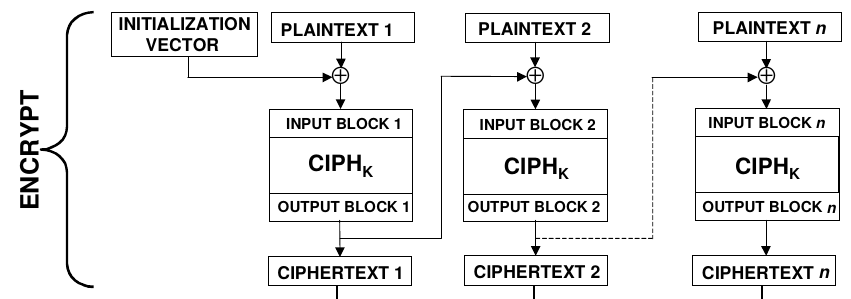
\includegraphics[width=\textwidth]{nist-cbc}
\caption{CBC encryption diagram}{The output of one block is used as the input of the next one. The decryption is very similar. Taken from the NIST recommendation~\cite{nist-sp800-38A}.}
\label{fig:cbc-encrypt}
\end{figure}

\begin{figure}
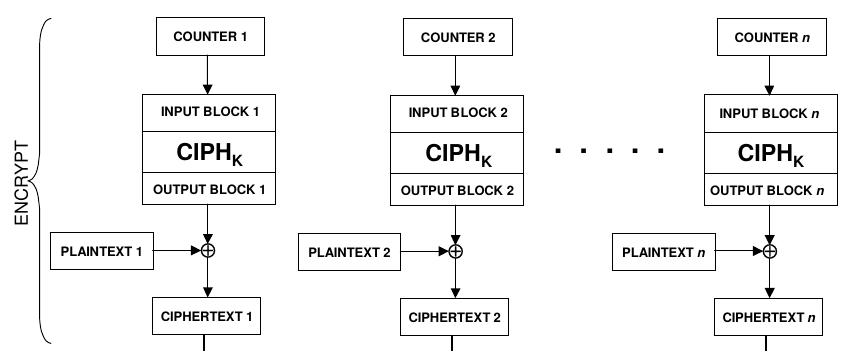
\includegraphics[width=\textwidth]{nist-ctr}
\caption{CTR encryption diagram}{Each block is processed independently from the others. The decryption is very similar. Taken from the NIST recommendation~\cite{nist-sp800-38A}.}
\label{fig:ctr-encrypt}
\end{figure}

Those modes can not work alone and have to be associated with a cipher (``CIPH" on figures~\ref{fig:cbc-encrypt}~and~\ref{fig:ctr-encrypt}).
In 1997, the NIST hosted a competition to choose the successor of the Data Encryption Standard (DES).
In 2000, Rijndael emerged victorious and was renamed Advanced Encryption Standard (AES).
It is still nowadays the most used symmetric block cipher used in a large variety of applications.\newline{}

Most applications want to use confidential and authenticated channels for their sensible communication.
In order to do so, they need to combine a symmetric cipher and a MAC.

\noindent New block cipher have emerged to answer the need for such combinations and formed the Authenticated Encryption with Associated Data (AEAD) mode of operation.
The most widespread mode in network applications is the Galois Counter Mode (GCM, see figure~\ref{fig:gcm-encrypt}), combining the CTR block cipher mode and a GHASH function using multiplications in the Galois field.
The advantage of this mode is that the authentication can be computed in parallel with the encryption, itself parallelizable.
This mode can thus be highly optimized in hardware, as proved Barco Silex with their BA415 IP core reaching up to 100Gbps~\cite{barco-ba415}.

\begin{figure}
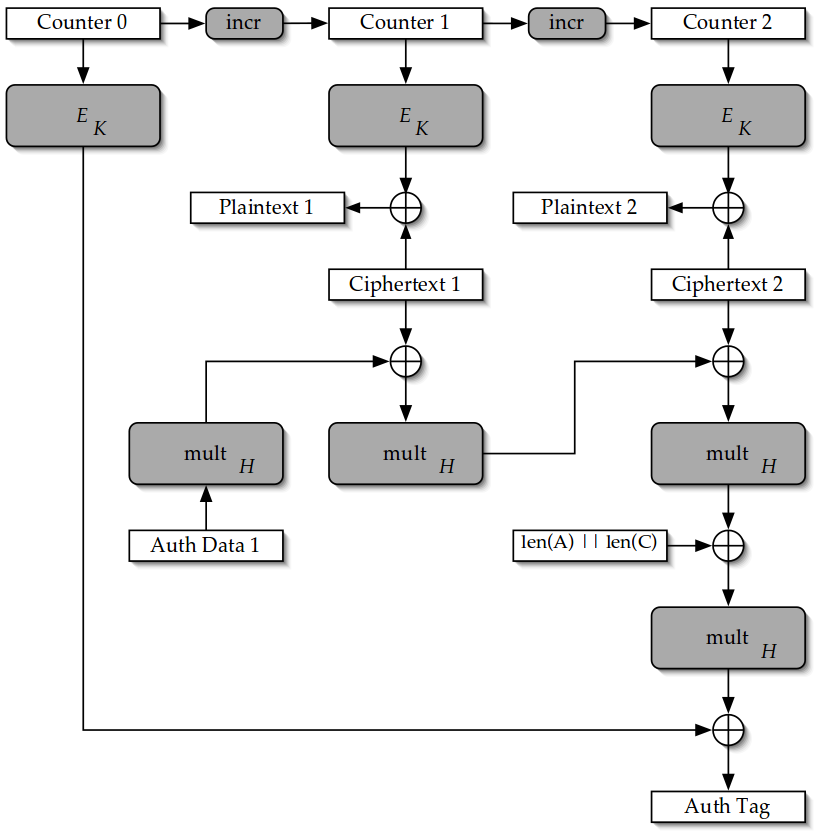
\includegraphics[width=\textwidth]{nist-gcm-encrypt}
\caption{GCM encryption diagram}{taken from the NIST specification~\cite{mcgrew2005}. The ciphertext blocks are formed by \textit{xor}-ing the encrypted counter and the plaintext. The tag is generated by a chain of ciphertext \textit{xor}-ing with Galois field multiplicated data. The decryption works excatly the same way, except the plaintext and ciphertext are swapped.}
\label{fig:gcm-encrypt}
\end{figure}









\subsection{Asymmetric cryptography}
Asymmetric cryptography relies on a pair of keys: one private known only to its owner, and one public available to anyone.
If we use the same notation for the cryptosystem as in section~\ref{sec:symmetric}, the public key would be $e$, and the private key $d$.
Such cryptography uses two kinds of operations: 
\begin{itemize}
	\item Encryption: the sender uses the public key of the recipient to encrypt the message $m$ into a ciphertext $c = E_e(m)$, and the recipient uses his private key to decrypt it: $m = D_d(m)$.
	\item Digital signature: the sender generates the signature $s$ of the message with his private key: $s = D_d(m)$, and the recipient uses the public key of the sender to verify the signature: $m = E_e(s)$.
	Since the sender can not deny having signed the message with his private key, this adds a non-repudiation of origin property to the scheme.
\end{itemize}

Eventhough the signature algorithms are often more efficient than the usual MACs and the key pairs key stay in use for very long period of time, asymmetric cryptography can not supplant its symmetric counterpart.
The throughput rates of modern asymmetric schemes are still well under the symmetric schemes, plus the key sizes are much larger.
Whereas the most efficient search for the symmetric key (ignoring the weaknesses specific to certain modes) is an exhaustive search, all public-key systems are vulnerable to more efficient attacks (\textit{e.g.} factorization or discrete logarithm).

In practice, public-key cryptography is used to estalish a secure channel between two or more peers and exchange a shared secret key that will be used the encrypt the subsequent communications.

\subsubsection{RSA}
RSA is a public-key scheme proposed in 1978 by three MIT researchers (who gave it their name)~\cite{Rivest:1978:MOD:359340.359342}.
A few years later, they founded RSA Laboratories, which is now in charge of maintaining its standards, alongside many others, as the first Public-Key Cryptography Standards, \textit{aka} PKCS \#1.
The last version of the standard is the version 2.2~\cite{pkcs1} and is defined as a precise key generation protocol allowing encryption and decryption.
The keys can be generated by respecting a few steps:
\begin{enumerate}
	\item randomy choose two large primes $p$ and $q$;
	\item compute the modulus $n = p q$, and consequently we have \[\phi(n) = (p-1)(q-1)\]with $\phi(n)$ as the Euler function;
	\item randomly choose the public exponent $e \in ]1,\phi(n)[\ s.t.\ GCD(e,\phi(n)) = 1$;
	\item compute $d \in ]1,\phi(n)[\ s.t.\ e \cdot d \equiv 1 (mod\ \phi(n))$
\end{enumerate}

With those parameters, we can form a public key with the pair $(n, e)$ and a private key with the pair $(n, d)$.

The encryption and decryption of a given message $m \in \mathds{Z}_n$ are defined as follows:
\begin{description}
	\item[Encryption] $c = m^e\ mod\ n$
	\item[Decryption] $m = c^d\ mod\ n$
\end{description}

The scheme is based on modular artihmetic, which is secure because of the factoring problem.
For an opponent to decrypt a ciphertext $c$ wihtout knowing the private key $(d, n)$, he would need to compute the $e^{th}$ roots of $c$, modulo $n$.
This operation is computationally hard, since an efficient solution is yet to be found for sufficiently large key size.


\subsubsection{Diffie-Hellman}
Diffie-Hellman is a secret key exchange protocol: two parties compute a shared secret $ZZ$ that can be used as a symmetric key during the following exchanges.
It uses the same kind of operation as RSA, that is modular exponentiation.
The protocol can be one of three types (\cite{rfc2631}, \cite{Frankel:2005:SGI:2206289}):
\begin{itemize}
	\item Static (DH): the actors use their authenticated certificate to compute the shared secret.
	\item Ephemeral (DHE): the actors create a new pair of public/private keys from which the secret key is derived.
	\item Anonymous: same as ephemeral, but without signing anything, hence not identifying neither of the actors, hence not providing any authentication. This mode is not advisable since it's vulnerable to main-in-the-middle attack.
\end{itemize}
A static scheme is easier to implement and requires much less operations, but using ephemeral keys is essential to ensure perfect forward secrecy.
Imagine that somehow, an opponent lays his hand on the shared secret.
If that secret has already been used, he can decipher all data transfered during past connections.
However, if the secret is new for every new connection, the compromission of the shared secret does not jeopardize past communications.
This is perfect forward secrecy: using a new key to protect the previous messages.

Hereunder is the generation algorithm of an ephemeral shared secret.
For a static secret, Alice and Bob will simply use their static certificate, sparing the modular exponentiation of the ephemeral public key generation.
\begin{enumerate}
	\item Alice generates once $p$ and $g$ (using precomputed parameters):
	\begin{description}[nosep]
		\item[p] large prime number
		\item[g] a generator of $\mathds{Z}_p^*$
	\end{description}
	\item Alice picks a random integer $x_a$ and computes $g^{x_a} mod\ p = y_a$.
	\item Alice sends $p$, $g$ and $y_a$ to Bob, signing everything using her private certificate.
	\item Bob checks the signature and picks $x_b$.
	\item Bob computes $y_a^{x_b} mod\ p = g^{x_a x_b} mod\ p = ZZ$, the shared secret to use as a premaster key from which will be derived the symmetric key for further communications.
	\item Bob sends $y_b = g^{x_b} mod\ p$, signing everything with his private certificate.
	\item Alice checks the signature and computes the same shared secret: $ZZ = y_b^{x_a} mod\ p = g^{x_a x_b} mod\ p$
\end{enumerate}

If the server is Alice, it has to do at least one signature generation, one signature verification and two modular exponentiations.
Note that the client, B in our case, could have one signature less because RFC 5246~\cite{rfc5246} leave it as an optional feature, and the server would then have one verification less.
However, any sane configuration will have both actors signing their ephemeral public key.
If the certificate use RSA, we end up with four modular exponentiations, which can become quite heavy computing wise for certain sizes of key.
We will see in chapter~\ref{chap:results} that while a 1024-bit key size is easily manageable by full software implementation, hardware offloading become a necessity for 4096-bit key sizes.
Moreover, 1024-bit parameter size, both RSA and Diffie-Hellman, are disallowed by the NIST recommandations since 2013~\cite{nist-sp800-131A}.












%%%%%%%%%%%%%%%%%%%%%%%%%%%%%%%%%%%%%%%%%%%%%%%%%%%%%%%%%%%%%%%%%%%%%%%%%%%%%%%%
\section{Network and VPN}\label{sec:theory-network}
%%%%%%%%%%%%%%%%%%%%%%%%%%%%%%%%%%%%%%%%%%%%%%%%%%%%%%%%%%%%%%%%%%%%%%%%%%%%%%%%

% Present the TCP/IP layering
Computer networks are described by two models: the TCP/IP stack and the OSI model, each splitting the network workflow into more or less abstract layers.
The RFC 1122~\cite{rfc1122} defines the TCP/IP, and the international standard ISO/IEC 7498-1~\cite{ISOIEC7498} defines the OSI stack as in the table~\ref{tab:tcp-ip-stack}.
The main difference between the two is the application layer of the TCP/IP stack which corresponds to the three upper layers of the OSI model.
Some references, such as~\citet{tanenbaum2011}, conceptually split the TCP/IP link layer into an additional physical layer.

\begin{table}[ht]
\center
\begin{tabularx}{\textwidth}{|l|l|l|X|} \hline
\multicolumn{2}{|c|}{TCP/IP layering} & \multicolumn{2}{c|}{OSI model} \\ \hline
Layer & Protocols & Layer & Protocols \\ \hline
\multirow{3}{*}{Application} & \multirow{3}{*}{FTP, SSH} & Application & FTP \\ \cline{3-4}
 & & Presentation & ASCII, JPEG \\ \cline{3-4}
 & & Session & RPC, PAP \\ \hline
Transport & TCP, UDP & Transport & TCP, UDP \\ \hline
Internet & IP, ICMP, IPsec & Network & IP, ICMP, IPsec \\ \hline
\multirow{2}{*}{Link} & \multirow{2}{*}{PPP, MAC, Ethernet, L2TP} & Data link & PPP, MAC, Ethernet, L2TP \\ \cline{3-4}
 & & Physical & USB, DSL, IEEE 802.11 \\ \hline
\end{tabularx}
\caption{TCP/IP and OSI model comparison}{They are globaly the same, except for the application layer of the TCP/IP stack which merge togheter the three upper layers of the OSI model. Between parenthsis are examples of protocols resting on each layer.}
\label{tab:tcp-ip-stack}
\end{table}


% First explain what a VPN is.
\citet{Frankel:2005:SGI:2206289} define a VPN as: ``virtual network built on top of existing physical networks that can provide a
secure communications mechanism for data and control information transmitted between networks."

There exist several major implementations of VPN: SSL, IPsec, L2TP and PPTP.
The later was developed by a vendor consortium leaded by Microsoft and proposed in the RFC 2637 and will not be discussed further.

\noindent L2TP (Layer 2 Tunneling Protocol) is a protocol that simply offers a tunnel without providing confidentiality~\cite{rfc3931}.
A common use case is to combine IPsec and L2TP, as defined in RFC 3193~\cite{rfc3193}.\newline{}

The present work will focus and SSL/TLS and IPsec, the figure~\ref{fig:ipsec-tls} showing their respective integration in the network stack.

\begin{figure}[ht]
\center
% Graphic for TeX using PGF
% Title: /home/para/documents/polytech2015/MA2/Master_thesis/master_thesis/tls-ipsec.dia
% Creator: Dia v0.97.3
% CreationDate: Thu May 28 14:34:18 2015
% For: para
% \usepackage{tikz}
% The following commands are not supported in PSTricks at present
% We define them conditionally, so when they are implemented,
% this pgf file will use them.
\ifx\du\undefined
  \newlength{\du}
\fi
\setlength{\du}{15\unitlength}
\begin{tikzpicture}
\pgftransformxscale{1.000000}
\pgftransformyscale{-1.000000}
\definecolor{dialinecolor}{rgb}{0.000000, 0.000000, 0.000000}
\pgfsetstrokecolor{dialinecolor}
\definecolor{dialinecolor}{rgb}{1.000000, 1.000000, 1.000000}
\pgfsetfillcolor{dialinecolor}
\pgfsetlinewidth{0.020000\du}
\pgfsetdash{}{0pt}
\pgfsetdash{}{0pt}
\pgfsetmiterjoin
\definecolor{dialinecolor}{rgb}{1.000000, 1.000000, 1.000000}
\pgfsetfillcolor{dialinecolor}
\fill (8.000000\du,3.500000\du)--(8.000000\du,4.100000\du)--(10.200000\du,4.100000\du)--(10.200000\du,3.500000\du)--cycle;
\definecolor{dialinecolor}{rgb}{0.000000, 0.000000, 0.000000}
\pgfsetstrokecolor{dialinecolor}
\draw (8.000000\du,3.500000\du)--(8.000000\du,4.100000\du)--(10.200000\du,4.100000\du)--(10.200000\du,3.500000\du)--cycle;
% setfont left to latex
\definecolor{dialinecolor}{rgb}{0.000000, 0.000000, 0.000000}
\pgfsetstrokecolor{dialinecolor}
\node at (9.100000\du,3.800000\du){Application};
\pgfsetlinewidth{0.020000\du}
\pgfsetdash{}{0pt}
\pgfsetdash{}{0pt}
\pgfsetmiterjoin
\definecolor{dialinecolor}{rgb}{1.000000, 1.000000, 1.000000}
\pgfsetfillcolor{dialinecolor}
\fill (8.000000\du,5.200000\du)--(8.000000\du,5.800000\du)--(10.200000\du,5.800000\du)--(10.200000\du,5.200000\du)--cycle;
\definecolor{dialinecolor}{rgb}{0.000000, 0.000000, 0.000000}
\pgfsetstrokecolor{dialinecolor}
\draw (8.000000\du,5.200000\du)--(8.000000\du,5.800000\du)--(10.200000\du,5.800000\du)--(10.200000\du,5.200000\du)--cycle;
% setfont left to latex
\definecolor{dialinecolor}{rgb}{0.000000, 0.000000, 0.000000}
\pgfsetstrokecolor{dialinecolor}
\node at (9.100000\du,5.500000\du){Transport};
\pgfsetlinewidth{0.020000\du}
\pgfsetdash{}{0pt}
\pgfsetdash{}{0pt}
\pgfsetmiterjoin
\definecolor{dialinecolor}{rgb}{1.000000, 1.000000, 1.000000}
\pgfsetfillcolor{dialinecolor}
\fill (8.000000\du,6.900000\du)--(8.000000\du,7.500000\du)--(10.200000\du,7.500000\du)--(10.200000\du,6.900000\du)--cycle;
\definecolor{dialinecolor}{rgb}{0.000000, 0.000000, 0.000000}
\pgfsetstrokecolor{dialinecolor}
\draw (8.000000\du,6.900000\du)--(8.000000\du,7.500000\du)--(10.200000\du,7.500000\du)--(10.200000\du,6.900000\du)--cycle;
% setfont left to latex
\definecolor{dialinecolor}{rgb}{0.000000, 0.000000, 0.000000}
\pgfsetstrokecolor{dialinecolor}
\node at (9.100000\du,7.200000\du){Internet};
\pgfsetlinewidth{0.020000\du}
\pgfsetdash{}{0pt}
\pgfsetdash{}{0pt}
\pgfsetmiterjoin
\definecolor{dialinecolor}{rgb}{1.000000, 1.000000, 1.000000}
\pgfsetfillcolor{dialinecolor}
\fill (8.000000\du,7.700000\du)--(8.000000\du,8.300000\du)--(10.200000\du,8.300000\du)--(10.200000\du,7.700000\du)--cycle;
\definecolor{dialinecolor}{rgb}{0.000000, 0.000000, 0.000000}
\pgfsetstrokecolor{dialinecolor}
\draw (8.000000\du,7.700000\du)--(8.000000\du,8.300000\du)--(10.200000\du,8.300000\du)--(10.200000\du,7.700000\du)--cycle;
% setfont left to latex
\definecolor{dialinecolor}{rgb}{0.000000, 0.000000, 0.000000}
\pgfsetstrokecolor{dialinecolor}
\node at (9.100000\du,8.000000\du){Link};
\pgfsetlinewidth{0.020000\du}
\pgfsetdash{}{0pt}
\pgfsetdash{}{0pt}
\pgfsetmiterjoin
\definecolor{dialinecolor}{rgb}{0.905882, 0.905882, 0.905882}
\pgfsetfillcolor{dialinecolor}
\fill (8.700000\du,4.300000\du)--(8.700000\du,4.900000\du)--(10.200000\du,4.900000\du)--(10.200000\du,4.300000\du)--cycle;
\definecolor{dialinecolor}{rgb}{0.000000, 0.000000, 0.000000}
\pgfsetstrokecolor{dialinecolor}
\draw (8.700000\du,4.300000\du)--(8.700000\du,4.900000\du)--(10.200000\du,4.900000\du)--(10.200000\du,4.300000\du)--cycle;
% setfont left to latex
\definecolor{dialinecolor}{rgb}{0.000000, 0.000000, 0.000000}
\pgfsetstrokecolor{dialinecolor}
\node at (9.450000\du,4.600000\du){SSL/TLS};
\pgfsetlinewidth{0.020000\du}
\pgfsetdash{}{0pt}
\pgfsetdash{}{0pt}
\pgfsetmiterjoin
\definecolor{dialinecolor}{rgb}{0.905882, 0.905882, 0.905882}
\pgfsetfillcolor{dialinecolor}
\fill (8.700000\du,6.000000\du)--(8.700000\du,6.600000\du)--(10.200000\du,6.600000\du)--(10.200000\du,6.000000\du)--cycle;
\definecolor{dialinecolor}{rgb}{0.000000, 0.000000, 0.000000}
\pgfsetstrokecolor{dialinecolor}
\draw (8.700000\du,6.000000\du)--(8.700000\du,6.600000\du)--(10.200000\du,6.600000\du)--(10.200000\du,6.000000\du)--cycle;
% setfont left to latex
\definecolor{dialinecolor}{rgb}{0.000000, 0.000000, 0.000000}
\pgfsetstrokecolor{dialinecolor}
\node at (9.450000\du,6.300000\du){IPsec};
\pgfsetlinewidth{0.050000\du}
\pgfsetdash{}{0pt}
\pgfsetdash{}{0pt}
\pgfsetbuttcap
{
\definecolor{dialinecolor}{rgb}{0.000000, 0.000000, 0.000000}
\pgfsetfillcolor{dialinecolor}
% was here!!!
\definecolor{dialinecolor}{rgb}{0.000000, 0.000000, 0.000000}
\pgfsetstrokecolor{dialinecolor}
\draw (9.450000\du,4.300000\du)--(9.450000\du,4.120000\du);
}
\pgfsetlinewidth{0.050000\du}
\pgfsetdash{}{0pt}
\pgfsetdash{}{0pt}
\pgfsetbuttcap
{
\definecolor{dialinecolor}{rgb}{0.000000, 0.000000, 0.000000}
\pgfsetfillcolor{dialinecolor}
% was here!!!
\definecolor{dialinecolor}{rgb}{0.000000, 0.000000, 0.000000}
\pgfsetstrokecolor{dialinecolor}
\draw (8.500000\du,4.120000\du)--(8.500000\du,5.180000\du);
}
\pgfsetlinewidth{0.050000\du}
\pgfsetdash{}{0pt}
\pgfsetdash{}{0pt}
\pgfsetbuttcap
{
\definecolor{dialinecolor}{rgb}{0.000000, 0.000000, 0.000000}
\pgfsetfillcolor{dialinecolor}
% was here!!!
\definecolor{dialinecolor}{rgb}{0.000000, 0.000000, 0.000000}
\pgfsetstrokecolor{dialinecolor}
\draw (8.500000\du,5.820000\du)--(8.500000\du,6.880000\du);
}
\pgfsetlinewidth{0.050000\du}
\pgfsetdash{}{0pt}
\pgfsetdash{}{0pt}
\pgfsetbuttcap
{
\definecolor{dialinecolor}{rgb}{0.000000, 0.000000, 0.000000}
\pgfsetfillcolor{dialinecolor}
% was here!!!
\definecolor{dialinecolor}{rgb}{0.000000, 0.000000, 0.000000}
\pgfsetstrokecolor{dialinecolor}
\draw (9.450000\du,6.000000\du)--(9.450000\du,5.820000\du);
}
\pgfsetlinewidth{0.050000\du}
\pgfsetdash{}{0pt}
\pgfsetdash{}{0pt}
\pgfsetbuttcap
{
\definecolor{dialinecolor}{rgb}{0.000000, 0.000000, 0.000000}
\pgfsetfillcolor{dialinecolor}
% was here!!!
\definecolor{dialinecolor}{rgb}{0.000000, 0.000000, 0.000000}
\pgfsetstrokecolor{dialinecolor}
\draw (9.450000\du,5.180000\du)--(9.450000\du,4.900000\du);
}
\pgfsetlinewidth{0.050000\du}
\pgfsetdash{}{0pt}
\pgfsetdash{}{0pt}
\pgfsetbuttcap
{
\definecolor{dialinecolor}{rgb}{0.000000, 0.000000, 0.000000}
\pgfsetfillcolor{dialinecolor}
% was here!!!
\definecolor{dialinecolor}{rgb}{0.000000, 0.000000, 0.000000}
\pgfsetstrokecolor{dialinecolor}
\draw (9.450000\du,6.880000\du)--(9.450000\du,6.600000\du);
}
\pgfsetlinewidth{0.050000\du}
\pgfsetdash{}{0pt}
\pgfsetdash{}{0pt}
\pgfsetbuttcap
{
\definecolor{dialinecolor}{rgb}{0.000000, 0.000000, 0.000000}
\pgfsetfillcolor{dialinecolor}
% was here!!!
\definecolor{dialinecolor}{rgb}{0.000000, 0.000000, 0.000000}
\pgfsetstrokecolor{dialinecolor}
\draw (9.100000\du,7.700000\du)--(9.100000\du,7.500000\du);
}
\pgfsetlinewidth{0.020000\du}
\pgfsetdash{}{0pt}
\pgfsetdash{}{0pt}
\pgfsetmiterjoin
\definecolor{dialinecolor}{rgb}{1.000000, 1.000000, 1.000000}
\pgfsetfillcolor{dialinecolor}
\fill (11.500000\du,3.500000\du)--(11.500000\du,4.100000\du)--(13.700000\du,4.100000\du)--(13.700000\du,3.500000\du)--cycle;
\definecolor{dialinecolor}{rgb}{0.000000, 0.000000, 0.000000}
\pgfsetstrokecolor{dialinecolor}
\draw (11.500000\du,3.500000\du)--(11.500000\du,4.100000\du)--(13.700000\du,4.100000\du)--(13.700000\du,3.500000\du)--cycle;
% setfont left to latex
\definecolor{dialinecolor}{rgb}{0.000000, 0.000000, 0.000000}
\pgfsetstrokecolor{dialinecolor}
\node at (12.600000\du,3.800000\du){Application};
\pgfsetlinewidth{0.020000\du}
\pgfsetdash{}{0pt}
\pgfsetdash{}{0pt}
\pgfsetmiterjoin
\definecolor{dialinecolor}{rgb}{1.000000, 1.000000, 1.000000}
\pgfsetfillcolor{dialinecolor}
\fill (11.500000\du,5.200000\du)--(11.500000\du,5.800000\du)--(13.700000\du,5.800000\du)--(13.700000\du,5.200000\du)--cycle;
\definecolor{dialinecolor}{rgb}{0.000000, 0.000000, 0.000000}
\pgfsetstrokecolor{dialinecolor}
\draw (11.500000\du,5.200000\du)--(11.500000\du,5.800000\du)--(13.700000\du,5.800000\du)--(13.700000\du,5.200000\du)--cycle;
% setfont left to latex
\definecolor{dialinecolor}{rgb}{0.000000, 0.000000, 0.000000}
\pgfsetstrokecolor{dialinecolor}
\node at (12.600000\du,5.500000\du){Transport};
\pgfsetlinewidth{0.020000\du}
\pgfsetdash{}{0pt}
\pgfsetdash{}{0pt}
\pgfsetmiterjoin
\definecolor{dialinecolor}{rgb}{1.000000, 1.000000, 1.000000}
\pgfsetfillcolor{dialinecolor}
\fill (11.500000\du,6.900000\du)--(11.500000\du,7.500000\du)--(13.700000\du,7.500000\du)--(13.700000\du,6.900000\du)--cycle;
\definecolor{dialinecolor}{rgb}{0.000000, 0.000000, 0.000000}
\pgfsetstrokecolor{dialinecolor}
\draw (11.500000\du,6.900000\du)--(11.500000\du,7.500000\du)--(13.700000\du,7.500000\du)--(13.700000\du,6.900000\du)--cycle;
% setfont left to latex
\definecolor{dialinecolor}{rgb}{0.000000, 0.000000, 0.000000}
\pgfsetstrokecolor{dialinecolor}
\node at (12.600000\du,7.200000\du){Internet};
\pgfsetlinewidth{0.020000\du}
\pgfsetdash{}{0pt}
\pgfsetdash{}{0pt}
\pgfsetmiterjoin
\definecolor{dialinecolor}{rgb}{1.000000, 1.000000, 1.000000}
\pgfsetfillcolor{dialinecolor}
\fill (11.500000\du,7.700000\du)--(11.500000\du,8.300000\du)--(13.700000\du,8.300000\du)--(13.700000\du,7.700000\du)--cycle;
\definecolor{dialinecolor}{rgb}{0.000000, 0.000000, 0.000000}
\pgfsetstrokecolor{dialinecolor}
\draw (11.500000\du,7.700000\du)--(11.500000\du,8.300000\du)--(13.700000\du,8.300000\du)--(13.700000\du,7.700000\du)--cycle;
% setfont left to latex
\definecolor{dialinecolor}{rgb}{0.000000, 0.000000, 0.000000}
\pgfsetstrokecolor{dialinecolor}
\node at (12.600000\du,8.000000\du){Link};
\pgfsetlinewidth{0.020000\du}
\pgfsetdash{}{0pt}
\pgfsetdash{}{0pt}
\pgfsetmiterjoin
\definecolor{dialinecolor}{rgb}{0.905882, 0.905882, 0.905882}
\pgfsetfillcolor{dialinecolor}
\fill (11.500000\du,4.300000\du)--(11.500000\du,4.900000\du)--(13.000000\du,4.900000\du)--(13.000000\du,4.300000\du)--cycle;
\definecolor{dialinecolor}{rgb}{0.000000, 0.000000, 0.000000}
\pgfsetstrokecolor{dialinecolor}
\draw (11.500000\du,4.300000\du)--(11.500000\du,4.900000\du)--(13.000000\du,4.900000\du)--(13.000000\du,4.300000\du)--cycle;
% setfont left to latex
\definecolor{dialinecolor}{rgb}{0.000000, 0.000000, 0.000000}
\pgfsetstrokecolor{dialinecolor}
\node at (12.250000\du,4.600000\du){SSL/TLS};
\pgfsetlinewidth{0.020000\du}
\pgfsetdash{}{0pt}
\pgfsetdash{}{0pt}
\pgfsetmiterjoin
\definecolor{dialinecolor}{rgb}{0.905882, 0.905882, 0.905882}
\pgfsetfillcolor{dialinecolor}
\fill (11.500000\du,6.000000\du)--(11.500000\du,6.600000\du)--(13.000000\du,6.600000\du)--(13.000000\du,6.000000\du)--cycle;
\definecolor{dialinecolor}{rgb}{0.000000, 0.000000, 0.000000}
\pgfsetstrokecolor{dialinecolor}
\draw (11.500000\du,6.000000\du)--(11.500000\du,6.600000\du)--(13.000000\du,6.600000\du)--(13.000000\du,6.000000\du)--cycle;
% setfont left to latex
\definecolor{dialinecolor}{rgb}{0.000000, 0.000000, 0.000000}
\pgfsetstrokecolor{dialinecolor}
\node at (12.250000\du,6.300000\du){IPsec};
\pgfsetlinewidth{0.050000\du}
\pgfsetdash{}{0pt}
\pgfsetdash{}{0pt}
\pgfsetbuttcap
{
\definecolor{dialinecolor}{rgb}{0.000000, 0.000000, 0.000000}
\pgfsetfillcolor{dialinecolor}
% was here!!!
\definecolor{dialinecolor}{rgb}{0.000000, 0.000000, 0.000000}
\pgfsetstrokecolor{dialinecolor}
\draw (12.250000\du,4.300000\du)--(12.250000\du,4.120000\du);
}
\pgfsetlinewidth{0.050000\du}
\pgfsetdash{}{0pt}
\pgfsetdash{}{0pt}
\pgfsetbuttcap
{
\definecolor{dialinecolor}{rgb}{0.000000, 0.000000, 0.000000}
\pgfsetfillcolor{dialinecolor}
% was here!!!
\definecolor{dialinecolor}{rgb}{0.000000, 0.000000, 0.000000}
\pgfsetstrokecolor{dialinecolor}
\draw (13.300000\du,4.120000\du)--(13.300000\du,5.180000\du);
}
\pgfsetlinewidth{0.050000\du}
\pgfsetdash{}{0pt}
\pgfsetdash{}{0pt}
\pgfsetbuttcap
{
\definecolor{dialinecolor}{rgb}{0.000000, 0.000000, 0.000000}
\pgfsetfillcolor{dialinecolor}
% was here!!!
\definecolor{dialinecolor}{rgb}{0.000000, 0.000000, 0.000000}
\pgfsetstrokecolor{dialinecolor}
\draw (13.300000\du,5.820000\du)--(13.300000\du,6.880000\du);
}
\pgfsetlinewidth{0.050000\du}
\pgfsetdash{}{0pt}
\pgfsetdash{}{0pt}
\pgfsetbuttcap
{
\definecolor{dialinecolor}{rgb}{0.000000, 0.000000, 0.000000}
\pgfsetfillcolor{dialinecolor}
% was here!!!
\definecolor{dialinecolor}{rgb}{0.000000, 0.000000, 0.000000}
\pgfsetstrokecolor{dialinecolor}
\draw (12.250000\du,6.000000\du)--(12.250000\du,5.820000\du);
}
\pgfsetlinewidth{0.050000\du}
\pgfsetdash{}{0pt}
\pgfsetdash{}{0pt}
\pgfsetbuttcap
{
\definecolor{dialinecolor}{rgb}{0.000000, 0.000000, 0.000000}
\pgfsetfillcolor{dialinecolor}
% was here!!!
\definecolor{dialinecolor}{rgb}{0.000000, 0.000000, 0.000000}
\pgfsetstrokecolor{dialinecolor}
\draw (12.250000\du,5.180000\du)--(12.250000\du,4.900000\du);
}
\pgfsetlinewidth{0.050000\du}
\pgfsetdash{}{0pt}
\pgfsetdash{}{0pt}
\pgfsetbuttcap
{
\definecolor{dialinecolor}{rgb}{0.000000, 0.000000, 0.000000}
\pgfsetfillcolor{dialinecolor}
% was here!!!
\definecolor{dialinecolor}{rgb}{0.000000, 0.000000, 0.000000}
\pgfsetstrokecolor{dialinecolor}
\draw (12.250000\du,6.880000\du)--(12.250000\du,6.600000\du);
}
\pgfsetlinewidth{0.050000\du}
\pgfsetdash{}{0pt}
\pgfsetdash{}{0pt}
\pgfsetbuttcap
{
\definecolor{dialinecolor}{rgb}{0.000000, 0.000000, 0.000000}
\pgfsetfillcolor{dialinecolor}
% was here!!!
\definecolor{dialinecolor}{rgb}{0.000000, 0.000000, 0.000000}
\pgfsetstrokecolor{dialinecolor}
\draw (12.600000\du,7.700000\du)--(12.600000\du,7.500000\du);
}
\pgfsetlinewidth{0.050000\du}
\pgfsetdash{}{0pt}
\pgfsetdash{}{0pt}
\pgfsetbuttcap
\pgfsetmiterjoin
\pgfsetlinewidth{0.000500\du}
\pgfsetbuttcap
\pgfsetmiterjoin
\pgfsetdash{}{0pt}
\definecolor{dialinecolor}{rgb}{0.000000, 0.588235, 0.831373}
\pgfsetfillcolor{dialinecolor}
\pgfpathmoveto{\pgfpoint{9.900000\du}{8.973111\du}}
\pgfpathlineto{\pgfpoint{9.900000\du}{9.289785\du}}
\pgfpathlineto{\pgfpoint{11.152729\du}{9.289785\du}}
\pgfpathlineto{\pgfpoint{11.152729\du}{8.973111\du}}
\pgfpathlineto{\pgfpoint{9.900000\du}{8.973111\du}}
\pgfusepath{fill}
\pgfsetbuttcap
\pgfsetmiterjoin
\pgfsetdash{}{0pt}
\definecolor{dialinecolor}{rgb}{0.666667, 0.901961, 1.000000}
\pgfsetstrokecolor{dialinecolor}
\pgfpathmoveto{\pgfpoint{9.900000\du}{8.973111\du}}
\pgfpathlineto{\pgfpoint{9.900000\du}{9.289785\du}}
\pgfpathlineto{\pgfpoint{11.152729\du}{9.289785\du}}
\pgfpathlineto{\pgfpoint{11.152729\du}{8.973111\du}}
\pgfpathlineto{\pgfpoint{9.900000\du}{8.973111\du}}
\pgfusepath{stroke}
\pgfsetbuttcap
\pgfsetmiterjoin
\pgfsetdash{}{0pt}
\definecolor{dialinecolor}{rgb}{0.000000, 0.352941, 0.501961}
\pgfsetfillcolor{dialinecolor}
\pgfpathmoveto{\pgfpoint{11.152729\du}{8.973111\du}}
\pgfpathlineto{\pgfpoint{11.540661\du}{8.600000\du}}
\pgfpathlineto{\pgfpoint{11.540661\du}{8.916674\du}}
\pgfpathlineto{\pgfpoint{11.152729\du}{9.289785\du}}
\pgfpathlineto{\pgfpoint{11.152729\du}{8.973111\du}}
\pgfusepath{fill}
\pgfsetbuttcap
\pgfsetmiterjoin
\pgfsetdash{}{0pt}
\definecolor{dialinecolor}{rgb}{0.666667, 0.901961, 1.000000}
\pgfsetstrokecolor{dialinecolor}
\pgfpathmoveto{\pgfpoint{11.152729\du}{8.973111\du}}
\pgfpathlineto{\pgfpoint{11.540661\du}{8.600000\du}}
\pgfpathlineto{\pgfpoint{11.540661\du}{8.916674\du}}
\pgfpathlineto{\pgfpoint{11.152729\du}{9.289785\du}}
\pgfpathlineto{\pgfpoint{11.152729\du}{8.973111\du}}
\pgfusepath{stroke}
\pgfsetbuttcap
\pgfsetmiterjoin
\pgfsetdash{}{0pt}
\definecolor{dialinecolor}{rgb}{0.000000, 0.705882, 1.000000}
\pgfsetfillcolor{dialinecolor}
\pgfpathmoveto{\pgfpoint{11.152729\du}{8.973111\du}}
\pgfpathlineto{\pgfpoint{11.540661\du}{8.600000\du}}
\pgfpathlineto{\pgfpoint{10.287077\du}{8.600000\du}}
\pgfpathlineto{\pgfpoint{9.900000\du}{8.973111\du}}
\pgfpathlineto{\pgfpoint{11.152729\du}{8.973111\du}}
\pgfusepath{fill}
\pgfsetbuttcap
\pgfsetmiterjoin
\pgfsetdash{}{0pt}
\definecolor{dialinecolor}{rgb}{0.666667, 0.901961, 1.000000}
\pgfsetstrokecolor{dialinecolor}
\pgfpathmoveto{\pgfpoint{11.152729\du}{8.973111\du}}
\pgfpathlineto{\pgfpoint{11.540661\du}{8.600000\du}}
\pgfpathlineto{\pgfpoint{10.287077\du}{8.600000\du}}
\pgfpathlineto{\pgfpoint{9.900000\du}{8.973111\du}}
\pgfpathlineto{\pgfpoint{11.152729\du}{8.973111\du}}
\pgfusepath{stroke}
\pgfsetbuttcap
\pgfsetmiterjoin
\pgfsetdash{}{0pt}
\definecolor{dialinecolor}{rgb}{0.000000, 0.000000, 0.000000}
\pgfsetfillcolor{dialinecolor}
\pgfpathmoveto{\pgfpoint{10.685556\du}{8.792399\du}}
\pgfpathlineto{\pgfpoint{10.640236\du}{8.836864\du}}
\pgfpathlineto{\pgfpoint{10.958905\du}{8.836864\du}}
\pgfpathlineto{\pgfpoint{10.913584\du}{8.893871\du}}
\pgfpathlineto{\pgfpoint{11.175531\du}{8.825748\du}}
\pgfpathlineto{\pgfpoint{11.039000\du}{8.769596\du}}
\pgfpathlineto{\pgfpoint{11.004510\du}{8.792399\du}}
\pgfpathlineto{\pgfpoint{10.685556\du}{8.792399\du}}
\pgfusepath{fill}
\pgfsetbuttcap
\pgfsetmiterjoin
\pgfsetdash{}{0pt}
\definecolor{dialinecolor}{rgb}{0.000000, 0.000000, 0.000000}
\pgfsetfillcolor{dialinecolor}
\pgfpathmoveto{\pgfpoint{10.845176\du}{8.645321\du}}
\pgfpathlineto{\pgfpoint{10.799570\du}{8.690356\du}}
\pgfpathlineto{\pgfpoint{11.118524\du}{8.690356\du}}
\pgfpathlineto{\pgfpoint{11.061517\du}{8.746793\du}}
\pgfpathlineto{\pgfpoint{11.334866\du}{8.668123\du}}
\pgfpathlineto{\pgfpoint{11.186933\du}{8.611116\du}}
\pgfpathlineto{\pgfpoint{11.164700\du}{8.645321\du}}
\pgfpathlineto{\pgfpoint{10.845176\du}{8.645321\du}}
\pgfusepath{fill}
\pgfsetbuttcap
\pgfsetmiterjoin
\pgfsetdash{}{0pt}
\definecolor{dialinecolor}{rgb}{0.000000, 0.000000, 0.000000}
\pgfsetfillcolor{dialinecolor}
\pgfpathmoveto{\pgfpoint{10.571542\du}{8.916674\du}}
\pgfpathlineto{\pgfpoint{10.618003\du}{8.871068\du}}
\pgfpathlineto{\pgfpoint{10.287077\du}{8.871068\du}}
\pgfpathlineto{\pgfpoint{10.344084\du}{8.814631\du}}
\pgfpathlineto{\pgfpoint{10.081567\du}{8.882185\du}}
\pgfpathlineto{\pgfpoint{10.218669\du}{8.939192\du}}
\pgfpathlineto{\pgfpoint{10.241757\du}{8.916674\du}}
\pgfpathlineto{\pgfpoint{10.571542\du}{8.916674\du}}
\pgfusepath{fill}
\pgfsetbuttcap
\pgfsetmiterjoin
\pgfsetdash{}{0pt}
\definecolor{dialinecolor}{rgb}{0.000000, 0.000000, 0.000000}
\pgfsetfillcolor{dialinecolor}
\pgfpathmoveto{\pgfpoint{10.720046\du}{8.757624\du}}
\pgfpathlineto{\pgfpoint{10.765651\du}{8.713444\du}}
\pgfpathlineto{\pgfpoint{10.446697\du}{8.713444\du}}
\pgfpathlineto{\pgfpoint{10.503989\du}{8.656437\du}}
\pgfpathlineto{\pgfpoint{10.230070\du}{8.735392\du}}
\pgfpathlineto{\pgfpoint{10.378004\du}{8.792399\du}}
\pgfpathlineto{\pgfpoint{10.400806\du}{8.757624\du}}
\pgfpathlineto{\pgfpoint{10.720046\du}{8.757624\du}}
\pgfusepath{fill}
\pgfsetbuttcap
\pgfsetmiterjoin
\pgfsetdash{}{0pt}
\definecolor{dialinecolor}{rgb}{1.000000, 1.000000, 1.000000}
\pgfsetfillcolor{dialinecolor}
\pgfpathmoveto{\pgfpoint{10.696958\du}{8.802945\du}}
\pgfpathlineto{\pgfpoint{10.651637\du}{8.848265\du}}
\pgfpathlineto{\pgfpoint{10.970591\du}{8.848265\du}}
\pgfpathlineto{\pgfpoint{10.924986\du}{8.904987\du}}
\pgfpathlineto{\pgfpoint{11.186933\du}{8.836864\du}}
\pgfpathlineto{\pgfpoint{11.049831\du}{8.780712\du}}
\pgfpathlineto{\pgfpoint{11.016197\du}{8.802945\du}}
\pgfpathlineto{\pgfpoint{10.696958\du}{8.802945\du}}
\pgfusepath{fill}
\pgfsetbuttcap
\pgfsetmiterjoin
\pgfsetdash{}{0pt}
\definecolor{dialinecolor}{rgb}{1.000000, 1.000000, 1.000000}
\pgfsetfillcolor{dialinecolor}
\pgfpathmoveto{\pgfpoint{10.856577\du}{8.656437\du}}
\pgfpathlineto{\pgfpoint{10.810972\du}{8.701472\du}}
\pgfpathlineto{\pgfpoint{11.129926\du}{8.701472\du}}
\pgfpathlineto{\pgfpoint{11.072919\du}{8.757624\du}}
\pgfpathlineto{\pgfpoint{11.346552\du}{8.678670\du}}
\pgfpathlineto{\pgfpoint{11.198619\du}{8.622518\du}}
\pgfpathlineto{\pgfpoint{11.175531\du}{8.656437\du}}
\pgfpathlineto{\pgfpoint{10.856577\du}{8.656437\du}}
\pgfusepath{fill}
\pgfsetbuttcap
\pgfsetmiterjoin
\pgfsetdash{}{0pt}
\definecolor{dialinecolor}{rgb}{1.000000, 1.000000, 1.000000}
\pgfsetfillcolor{dialinecolor}
\pgfpathmoveto{\pgfpoint{10.582944\du}{8.927790\du}}
\pgfpathlineto{\pgfpoint{10.628549\du}{8.882185\du}}
\pgfpathlineto{\pgfpoint{10.298764\du}{8.882185\du}}
\pgfpathlineto{\pgfpoint{10.354916\du}{8.825748\du}}
\pgfpathlineto{\pgfpoint{10.093254\du}{8.893871\du}}
\pgfpathlineto{\pgfpoint{10.230070\du}{8.950308\du}}
\pgfpathlineto{\pgfpoint{10.252588\du}{8.927790\du}}
\pgfpathlineto{\pgfpoint{10.582944\du}{8.927790\du}}
\pgfusepath{fill}
\pgfsetbuttcap
\pgfsetmiterjoin
\pgfsetdash{}{0pt}
\definecolor{dialinecolor}{rgb}{1.000000, 1.000000, 1.000000}
\pgfsetfillcolor{dialinecolor}
\pgfpathmoveto{\pgfpoint{10.730877\du}{8.769596\du}}
\pgfpathlineto{\pgfpoint{10.777053\du}{8.723990\du}}
\pgfpathlineto{\pgfpoint{10.457528\du}{8.723990\du}}
\pgfpathlineto{\pgfpoint{10.514820\du}{8.668123\du}}
\pgfpathlineto{\pgfpoint{10.241757\du}{8.746793\du}}
\pgfpathlineto{\pgfpoint{10.389690\du}{8.802945\du}}
\pgfpathlineto{\pgfpoint{10.411923\du}{8.769596\du}}
\pgfpathlineto{\pgfpoint{10.730877\du}{8.769596\du}}
\pgfusepath{fill}
\pgfsetlinewidth{0.050000\du}
\pgfsetdash{}{0pt}
\pgfsetdash{}{0pt}
\pgfsetmiterjoin
\pgfsetbuttcap
{
\definecolor{dialinecolor}{rgb}{0.000000, 0.000000, 0.000000}
\pgfsetfillcolor{dialinecolor}
% was here!!!
{\pgfsetcornersarced{\pgfpoint{0.000000\du}{0.000000\du}}\definecolor{dialinecolor}{rgb}{0.000000, 0.000000, 0.000000}
\pgfsetstrokecolor{dialinecolor}
\draw (9.100000\du,8.300000\du)--(9.100000\du,8.973111\du)--(9.900000\du,8.973111\du);
}}
\pgfsetlinewidth{0.050000\du}
\pgfsetdash{}{0pt}
\pgfsetdash{}{0pt}
\pgfsetmiterjoin
\pgfsetbuttcap
{
\definecolor{dialinecolor}{rgb}{0.000000, 0.000000, 0.000000}
\pgfsetfillcolor{dialinecolor}
% was here!!!
{\pgfsetcornersarced{\pgfpoint{0.000000\du}{0.000000\du}}\definecolor{dialinecolor}{rgb}{0.000000, 0.000000, 0.000000}
\pgfsetstrokecolor{dialinecolor}
\draw (12.600000\du,8.300000\du)--(12.600000\du,8.916674\du)--(11.540661\du,8.916674\du);
}}
\end{tikzpicture}

\caption{SSL/TLS and IPsec integration into the TCP/IP network stack}{SSL/TLS works in the application layer in order to secure the transport layer, whilst IPsec secures the Internet layer.}
\label{fig:tls-ipsec}
\end{figure}

\subsection{SSL/TLS}
% Introduce SSL/TLS, talk about the protocol, the key exchange and stuff, but leaver OpenVPN for the 'implementation' chapter.
% Question the security? Apparently, it does mac-then-encrypt, which is insecure regarding certain types of attacks \cite{cryptoeprint:2001:045}.
% Plus, SSLv3 is to be deprecated, according to a queued RFC: http://www.rfc-editor.org/internet-drafts/draft-ietf-tls-sslv3-diediedie-03.txt, and is not supported anymore by many servers since poodle.
Secure Socket Layer (SSL) and Transport Layer Security (TLS) are two protocols ensuring secure communications from the application layer, securing the transport layer.
The last version of SSL (version 3.0) dates from 1996~\cite{rfc6101} and has been found a critical vulnerability by Google in 2014~\cite{poodle}.
As a consequence, SSL 3.0 support is being dropped, and the IETF is working on a depracation of the standard~\cite{sslv3-diediedie-03}.

\noindent TLS is the successor of SSL is at version 1.2~\cite{rfc5246}, the next version being developed by the IETF~\cite{tls13-05}.
TLS uses X.509 certificates for the asymmetric cryptography used during the key exchange.
Those certificates come in pair: one public and a second private, and rely on a chain of trust for the validity of the certificate.
Usually, the term certificate is use for the public certificate, and private key for the corresponding private certificate.

\noindent The figure~\ref{fig:tls-handshake} shows the messages exchanged during the establishement of a connection between two peers.


\begin{figure}[ht]
\begin{verbatim}
Client                                             Server

ClientHello                -------->
                                              ServerHello
                                             Certificate*
                                       ServerKeyExchange*
                                      CertificateRequest*
                           <--------      ServerHelloDone
Certificate*
ClientKeyExchange
CertificateVerify*
[ChangeCipherSpec]
Finished                   -------->
                                       [ChangeCipherSpec]
                           <--------             Finished
Application Data           <------->     Application Data
\end{verbatim}
\caption{TLS handshake}{The * denotes messages that are sent only in some situations. Reproduce from~\cite{rfc5246}.}
\label{fig:tls-handshake}
\end{figure}

\begin{enumerate}
	\item Client: ClientHello. The client sends a series of specifications to the server, such as the protocol version and the supported cipher suites.
	\item Server: ServerHello and others. The server replies by setting the protocol and the cipher suite to use.
	It can send its own certificate and request the client's.
	In some cases, the server can already begin the key echange protocol (\textit{e.g.} Diffie-Hellman).
	\item Client: ClientKeyExchange and others. The client veryfies the validity of the server certificate, if any, and sends its own. If necessary, the client may have to change its cipher specification based on the constraints of the server, or request a new specification from the server.
	The client can also participate in the key exchange protocol.
	\item Server: Finished. If the client asked for a new cipher specification, the server can set a new one. Otherwise, the exchange is simply finished and the connection has been successfully established.
\end{enumerate}

Once the connection is established, the peers can exchange application data using the symmetric key negociated during the handshake.








\subsection{IPsec}
% IPsec as a protocol, strongswan come in the 'implementation' chapter.
IPsec is a protocol whose implementation is a modification of the IP stack in the kernel space.
It is a network/internet level security; it examines incomming IP packets and checks if there exists a security association with the destination, and decrypt it on-the-fly if necessary.

% One of the main disadvantage compared to a user-space VPN is the difficulty to traverse NAT.

IPsec consist of three components~\cite{cryptoencyclopedia2011}, each defined in their respective RFC:
\begin{description}
	\item[Traffic protocols] Encapsulating Security Payload (ESP,~\cite{rfc4303}) and Authentication Header (AH,~\cite{rfc4302}).
	\item[Key management] Internet Key Exchange (IKEv2,~\cite{rfc7296}).
	\item[Policy]Security Policy Database (SPD,~\cite{rfc4301}) and Security Association (SA~\cite{rfc4301}).
\end{description}

As~\citet{Paterson200672} present them, the SAs are used as repository for cryptographic parameters, and the SPD defines the policies to apply.
If the SPD can be populated by hand, typically in a configuration file, the SA management should be left to an automated mechanism: the IKEv2.

\noindent The IKEv2 protocol uses four different types of exchanges to fulfill its role:
\begin{itemize}
	\item \texttt{IKE\_SA\_INIT}: The two peers agree on cryptographic parameters to use. Among these is a Diffie-Hellman shared secret from which are derived symmetric keys used for a special IKE SA.
	\item \texttt{IKE\_AUTH}: Once the peers are protected by the IKE SA, they can authenticate themselves to each other and add a first SA in the SA database (SADB).
	The protocol supports three types of authentication methods:
	\begin{itemize}
		\item Digital signature using a PKI.
		\item MAC using a pre-established secret key.
		\item Extensible Authentication Protocol (EAP) defined in~\citet{rfc3748}.
	\end{itemize}
	At this point, the connection is fully established and ready to use.
	\item \texttt{CREATE\_CHILD\_SA}: Used to create new SAs between the two peers. It may involve new generations of DH secrets to ensure perfect forward secrecy.
	\item \texttt{INFORMATIONAL}: Exchange of management information.
\end{itemize}
~\newline{}

The figure~\ref{fig:esp-packet-structure} shows the structure of an ESP packet.
The ESP header includes two fields: a Security Parameter Index (SPI) and a Sequence Number (SN)
The SPI is a value on which both actors agreed on during the key exchange protocol, identifying the SA to use for the communication.
The SN is an anti-replay feature, an integer incrementing with each packet processed by the SA. This way, the SA will reject any packet that does not have a SN in the current windows, avoiding an intruder to resend a previously captured packet on the network.
As the SN is covered by the integrity, the opponent can not change it without having to change the Integrity Check Value (ICV, \textit{a.k.a.} the message digest).
This authentication covers the whole packet, whilst the confidentiality excludes the ESP header.

\noindent The ESP trailer includes a padding and two 1-byte fields: the padding length and the next header value, which can specify if the packet is dummy or real.
The padding is needed when using block ciphers to obtain a payload which length is an integral multiple of the block length.

\noindent The ESP payload includes an optional IV and an optional Traffic Flow Confidentiality (TFC) padding.
The TFC padding allows to modify the length of the packet with dummy data, somewhat hiding the true nature of the payload.
It differs from the standard padding because its length is not limited to 255 bytes like the latter.

\noindent AH is the same as ESP, except is does not offer encryption features, only the authentication.
Since ESP can use a null cipher, it arguably offers the same features as AH.
The existance of AH is actually historical; when the protocol was developed in the 1990s, there were laws in the United States and other countries preventing the export of product including encryption features.
Having an authentication only counterparty allowed such product to be exported without encryption capabilities.\newline{}

IPsec can be deployed in two modes: 
\begin{itemize}
	\item Transport for end-to-end service and protecting the payload. IPsec examines the incomming payload, checks it has not been tampered with and pass it to the next layer.
	\item Tunnel protects the entire IP packet by encapsulating it into a new IP packet. As the destination contained in the new IP header can be different from the original, this mode can be used to manage gateways.
\end{itemize}
The figure~\ref{fig:ipsec-transport-tunnel} shows the space overhead imposed by AH and ESP in transport and tunnel modes.

Both protocols add 10 bytes of fixed size fields (SPI, SN, pad length and next header).
The other fields are of variable length, or even optional, such as the optional authentication field of minimum 12 bytes, the optional IV of minimum 4 bytes and the padding between 0 and 255 bytes long.
\citet{Xenakis20063225} reached the conclusion in their paper that the use of lightweight -- and deprecated -- encryption schemes (\textit{e.g.} HMAC-MD5 and DES) hardly had any impact on the throughput of the system and on the delay of the packets.
Hence, the space overhead of IPsec is negligible when using more serious schemes (\textit{e.g.} AES-256-CBC with HMAC-SHA-256).


\begin{figure}[ht]
\center
\subfloat[\label{fig:ipsec-transport}Transport]{%
	\large
	\resizebox{.465\linewidth}{!}{%
	% Graphic for TeX using PGF
% Title: /home/para/documents/polytech2015/MA2/Master_thesis/master_thesis/ipsec-transport.dia
% Creator: Dia v0.97.3
% CreationDate: Thu May 21 00:33:06 2015
% For: para
% \usepackage{tikz}
% The following commands are not supported in PSTricks at present
% We define them conditionally, so when they are implemented,
% this pgf file will use them.
\ifx\du\undefined
  \newlength{\du}
\fi
\setlength{\du}{15\unitlength}
\begin{tikzpicture}
\pgftransformxscale{1.000000}
\pgftransformyscale{-1.000000}
\definecolor{dialinecolor}{rgb}{0.000000, 0.000000, 0.000000}
\pgfsetstrokecolor{dialinecolor}
\definecolor{dialinecolor}{rgb}{1.000000, 1.000000, 1.000000}
\pgfsetfillcolor{dialinecolor}
\pgfsetlinewidth{0.050000\du}
\pgfsetdash{}{0pt}
\pgfsetdash{}{0pt}
\pgfsetmiterjoin
\definecolor{dialinecolor}{rgb}{1.000000, 1.000000, 1.000000}
\pgfsetfillcolor{dialinecolor}
\fill (17.500000\du,15.100000\du)--(17.500000\du,16.100000\du)--(19.000000\du,16.100000\du)--(19.000000\du,15.100000\du)--cycle;
\definecolor{dialinecolor}{rgb}{0.000000, 0.000000, 0.000000}
\pgfsetstrokecolor{dialinecolor}
\draw (17.500000\du,15.100000\du)--(17.500000\du,16.100000\du)--(19.000000\du,16.100000\du)--(19.000000\du,15.100000\du)--cycle;
\pgfsetlinewidth{0.050000\du}
\pgfsetdash{}{0pt}
\pgfsetdash{}{0pt}
\pgfsetmiterjoin
\definecolor{dialinecolor}{rgb}{1.000000, 1.000000, 1.000000}
\pgfsetfillcolor{dialinecolor}
\fill (17.000000\du,13.400000\du)--(17.000000\du,14.400000\du)--(19.000000\du,14.400000\du)--(19.000000\du,13.400000\du)--cycle;
\definecolor{dialinecolor}{rgb}{0.000000, 0.000000, 0.000000}
\pgfsetstrokecolor{dialinecolor}
\draw (17.000000\du,13.400000\du)--(17.000000\du,14.400000\du)--(19.000000\du,14.400000\du)--(19.000000\du,13.400000\du)--cycle;
\pgfsetlinewidth{0.050000\du}
\pgfsetdash{}{0pt}
\pgfsetdash{}{0pt}
\pgfsetmiterjoin
\definecolor{dialinecolor}{rgb}{1.000000, 1.000000, 1.000000}
\pgfsetfillcolor{dialinecolor}
\fill (16.000000\du,11.700000\du)--(16.000000\du,12.700000\du)--(18.000000\du,12.700000\du)--(18.000000\du,11.700000\du)--cycle;
\definecolor{dialinecolor}{rgb}{0.000000, 0.000000, 0.000000}
\pgfsetstrokecolor{dialinecolor}
\draw (16.000000\du,11.700000\du)--(16.000000\du,12.700000\du)--(18.000000\du,12.700000\du)--(18.000000\du,11.700000\du)--cycle;
\pgfsetlinewidth{0.050000\du}
\pgfsetdash{}{0pt}
\pgfsetdash{}{0pt}
\pgfsetmiterjoin
\definecolor{dialinecolor}{rgb}{1.000000, 1.000000, 1.000000}
\pgfsetfillcolor{dialinecolor}
\fill (14.000000\du,10.000000\du)--(14.000000\du,11.000000\du)--(16.000000\du,11.000000\du)--(16.000000\du,10.000000\du)--cycle;
\definecolor{dialinecolor}{rgb}{0.000000, 0.000000, 0.000000}
\pgfsetstrokecolor{dialinecolor}
\draw (14.000000\du,10.000000\du)--(14.000000\du,11.000000\du)--(16.000000\du,11.000000\du)--(16.000000\du,10.000000\du)--cycle;
\pgfsetlinewidth{0.050000\du}
\pgfsetdash{}{0pt}
\pgfsetdash{}{0pt}
\pgfsetmiterjoin
\definecolor{dialinecolor}{rgb}{1.000000, 1.000000, 1.000000}
\pgfsetfillcolor{dialinecolor}
\fill (10.000000\du,10.000000\du)--(10.000000\du,11.000000\du)--(12.000000\du,11.000000\du)--(12.000000\du,10.000000\du)--cycle;
\definecolor{dialinecolor}{rgb}{0.000000, 0.000000, 0.000000}
\pgfsetstrokecolor{dialinecolor}
\draw (10.000000\du,10.000000\du)--(10.000000\du,11.000000\du)--(12.000000\du,11.000000\du)--(12.000000\du,10.000000\du)--cycle;
% setfont left to latex
\definecolor{dialinecolor}{rgb}{0.000000, 0.000000, 0.000000}
\pgfsetstrokecolor{dialinecolor}
\node at (11.000000\du,10.500000\du){Payload};
\pgfsetlinewidth{0.050000\du}
\pgfsetdash{}{0pt}
\pgfsetdash{}{0pt}
\pgfsetmiterjoin
\definecolor{dialinecolor}{rgb}{1.000000, 1.000000, 1.000000}
\pgfsetfillcolor{dialinecolor}
\fill (12.000000\du,10.000000\du)--(12.000000\du,11.000000\du)--(14.000000\du,11.000000\du)--(14.000000\du,10.000000\du)--cycle;
\definecolor{dialinecolor}{rgb}{0.000000, 0.000000, 0.000000}
\pgfsetstrokecolor{dialinecolor}
\draw (12.000000\du,10.000000\du)--(12.000000\du,11.000000\du)--(14.000000\du,11.000000\du)--(14.000000\du,10.000000\du)--cycle;
% setfont left to latex
\definecolor{dialinecolor}{rgb}{0.000000, 0.000000, 0.000000}
\pgfsetstrokecolor{dialinecolor}
\node at (15.000000\du,10.500000\du){IP hdr};
% setfont left to latex
\definecolor{dialinecolor}{rgb}{0.000000, 0.000000, 0.000000}
\pgfsetstrokecolor{dialinecolor}
\node at (13.000000\du,10.500000\du){TCP hdr};
\pgfsetlinewidth{0.050000\du}
\pgfsetdash{}{0pt}
\pgfsetdash{}{0pt}
\pgfsetmiterjoin
\definecolor{dialinecolor}{rgb}{1.000000, 1.000000, 1.000000}
\pgfsetfillcolor{dialinecolor}
\fill (10.000000\du,11.700000\du)--(10.000000\du,12.700000\du)--(12.000000\du,12.700000\du)--(12.000000\du,11.700000\du)--cycle;
\definecolor{dialinecolor}{rgb}{0.000000, 0.000000, 0.000000}
\pgfsetstrokecolor{dialinecolor}
\draw (10.000000\du,11.700000\du)--(10.000000\du,12.700000\du)--(12.000000\du,12.700000\du)--(12.000000\du,11.700000\du)--cycle;
% setfont left to latex
\definecolor{dialinecolor}{rgb}{0.000000, 0.000000, 0.000000}
\pgfsetstrokecolor{dialinecolor}
\node at (11.000000\du,12.200000\du){Payload};
\pgfsetlinewidth{0.050000\du}
\pgfsetdash{}{0pt}
\pgfsetdash{}{0pt}
\pgfsetmiterjoin
\definecolor{dialinecolor}{rgb}{1.000000, 1.000000, 1.000000}
\pgfsetfillcolor{dialinecolor}
\fill (12.000000\du,11.700000\du)--(12.000000\du,12.700000\du)--(14.000000\du,12.700000\du)--(14.000000\du,11.700000\du)--cycle;
\definecolor{dialinecolor}{rgb}{0.000000, 0.000000, 0.000000}
\pgfsetstrokecolor{dialinecolor}
\draw (12.000000\du,11.700000\du)--(12.000000\du,12.700000\du)--(14.000000\du,12.700000\du)--(14.000000\du,11.700000\du)--cycle;
% setfont left to latex
\definecolor{dialinecolor}{rgb}{0.000000, 0.000000, 0.000000}
\pgfsetstrokecolor{dialinecolor}
\node at (17.000000\du,12.200000\du){IP hdr};
% setfont left to latex
\definecolor{dialinecolor}{rgb}{0.000000, 0.000000, 0.000000}
\pgfsetstrokecolor{dialinecolor}
\node at (13.000000\du,12.200000\du){TCP hdr};
\pgfsetlinewidth{0.050000\du}
\pgfsetdash{}{0pt}
\pgfsetdash{}{0pt}
\pgfsetmiterjoin
\definecolor{dialinecolor}{rgb}{1.000000, 1.000000, 1.000000}
\pgfsetfillcolor{dialinecolor}
\fill (14.000000\du,11.700000\du)--(14.000000\du,12.700000\du)--(16.000000\du,12.700000\du)--(16.000000\du,11.700000\du)--cycle;
\definecolor{dialinecolor}{rgb}{0.000000, 0.000000, 0.000000}
\pgfsetstrokecolor{dialinecolor}
\draw (14.000000\du,11.700000\du)--(14.000000\du,12.700000\du)--(16.000000\du,12.700000\du)--(16.000000\du,11.700000\du)--cycle;
% setfont left to latex
\definecolor{dialinecolor}{rgb}{0.000000, 0.000000, 0.000000}
\pgfsetstrokecolor{dialinecolor}
\node at (15.000000\du,12.200000\du){AH hdr};
% setfont left to latex
\definecolor{dialinecolor}{rgb}{0.000000, 0.000000, 0.000000}
\pgfsetstrokecolor{dialinecolor}
\node[anchor=west] at (10.500000\du,9.800000\du){Original IP};
% setfont left to latex
\definecolor{dialinecolor}{rgb}{0.000000, 0.000000, 0.000000}
\pgfsetstrokecolor{dialinecolor}
\node[anchor=west] at (10.500000\du,11.500000\du){AH protocol, authentication};
\pgfsetlinewidth{0.050000\du}
\pgfsetdash{}{0pt}
\pgfsetdash{}{0pt}
\pgfsetmiterjoin
\definecolor{dialinecolor}{rgb}{1.000000, 1.000000, 1.000000}
\pgfsetfillcolor{dialinecolor}
\fill (11.000000\du,13.400000\du)--(11.000000\du,14.400000\du)--(13.000000\du,14.400000\du)--(13.000000\du,13.400000\du)--cycle;
\definecolor{dialinecolor}{rgb}{0.000000, 0.000000, 0.000000}
\pgfsetstrokecolor{dialinecolor}
\draw (11.000000\du,13.400000\du)--(11.000000\du,14.400000\du)--(13.000000\du,14.400000\du)--(13.000000\du,13.400000\du)--cycle;
% setfont left to latex
\definecolor{dialinecolor}{rgb}{0.000000, 0.000000, 0.000000}
\pgfsetstrokecolor{dialinecolor}
\node at (12.000000\du,13.900000\du){Payload};
\pgfsetlinewidth{0.050000\du}
\pgfsetdash{}{0pt}
\pgfsetdash{}{0pt}
\pgfsetmiterjoin
\definecolor{dialinecolor}{rgb}{1.000000, 1.000000, 1.000000}
\pgfsetfillcolor{dialinecolor}
\fill (13.000000\du,13.400000\du)--(13.000000\du,14.400000\du)--(15.000000\du,14.400000\du)--(15.000000\du,13.400000\du)--cycle;
\definecolor{dialinecolor}{rgb}{0.000000, 0.000000, 0.000000}
\pgfsetstrokecolor{dialinecolor}
\draw (13.000000\du,13.400000\du)--(13.000000\du,14.400000\du)--(15.000000\du,14.400000\du)--(15.000000\du,13.400000\du)--cycle;
% setfont left to latex
\definecolor{dialinecolor}{rgb}{0.000000, 0.000000, 0.000000}
\pgfsetstrokecolor{dialinecolor}
\node at (18.000000\du,13.900000\du){IP hdr};
% setfont left to latex
\definecolor{dialinecolor}{rgb}{0.000000, 0.000000, 0.000000}
\pgfsetstrokecolor{dialinecolor}
\node at (14.000000\du,13.900000\du){TCP hdr};
\pgfsetlinewidth{0.050000\du}
\pgfsetdash{}{0pt}
\pgfsetdash{}{0pt}
\pgfsetmiterjoin
\definecolor{dialinecolor}{rgb}{1.000000, 1.000000, 1.000000}
\pgfsetfillcolor{dialinecolor}
\fill (15.000000\du,13.400000\du)--(15.000000\du,14.400000\du)--(17.000000\du,14.400000\du)--(17.000000\du,13.400000\du)--cycle;
\definecolor{dialinecolor}{rgb}{0.000000, 0.000000, 0.000000}
\pgfsetstrokecolor{dialinecolor}
\draw (15.000000\du,13.400000\du)--(15.000000\du,14.400000\du)--(17.000000\du,14.400000\du)--(17.000000\du,13.400000\du)--cycle;
% setfont left to latex
\definecolor{dialinecolor}{rgb}{0.000000, 0.000000, 0.000000}
\pgfsetstrokecolor{dialinecolor}
\node at (16.000000\du,13.900000\du){ESP hdr};
\pgfsetlinewidth{0.050000\du}
\pgfsetdash{}{0pt}
\pgfsetdash{}{0pt}
\pgfsetmiterjoin
\definecolor{dialinecolor}{rgb}{1.000000, 1.000000, 1.000000}
\pgfsetfillcolor{dialinecolor}
\fill (10.000000\du,13.400000\du)--(10.000000\du,14.400000\du)--(11.000000\du,14.400000\du)--(11.000000\du,13.400000\du)--cycle;
\definecolor{dialinecolor}{rgb}{0.000000, 0.000000, 0.000000}
\pgfsetstrokecolor{dialinecolor}
\draw (10.000000\du,13.400000\du)--(10.000000\du,14.400000\du)--(11.000000\du,14.400000\du)--(11.000000\du,13.400000\du)--cycle;
% setfont left to latex
\definecolor{dialinecolor}{rgb}{0.000000, 0.000000, 0.000000}
\pgfsetstrokecolor{dialinecolor}
\node at (10.500000\du,13.804583\du){ESP};
% setfont left to latex
\definecolor{dialinecolor}{rgb}{0.000000, 0.000000, 0.000000}
\pgfsetstrokecolor{dialinecolor}
\node at (10.500000\du,14.227917\du){trl};
% setfont left to latex
\definecolor{dialinecolor}{rgb}{0.000000, 0.000000, 0.000000}
\pgfsetstrokecolor{dialinecolor}
\node[anchor=west] at (10.500000\du,13.200000\du){ESP protocol, confidentiality};
\pgfsetlinewidth{0.050000\du}
\pgfsetdash{}{0pt}
\pgfsetdash{}{0pt}
\pgfsetmiterjoin
\definecolor{dialinecolor}{rgb}{1.000000, 1.000000, 1.000000}
\pgfsetfillcolor{dialinecolor}
\fill (12.500000\du,15.100000\du)--(12.500000\du,16.100000\du)--(14.500000\du,16.100000\du)--(14.500000\du,15.100000\du)--cycle;
\definecolor{dialinecolor}{rgb}{0.000000, 0.000000, 0.000000}
\pgfsetstrokecolor{dialinecolor}
\draw (12.500000\du,15.100000\du)--(12.500000\du,16.100000\du)--(14.500000\du,16.100000\du)--(14.500000\du,15.100000\du)--cycle;
% setfont left to latex
\definecolor{dialinecolor}{rgb}{0.000000, 0.000000, 0.000000}
\pgfsetstrokecolor{dialinecolor}
\node at (13.500000\du,15.600000\du){Payload};
\pgfsetlinewidth{0.050000\du}
\pgfsetdash{}{0pt}
\pgfsetdash{}{0pt}
\pgfsetmiterjoin
\definecolor{dialinecolor}{rgb}{1.000000, 1.000000, 1.000000}
\pgfsetfillcolor{dialinecolor}
\fill (14.500000\du,15.100000\du)--(14.500000\du,16.100000\du)--(16.000000\du,16.100000\du)--(16.000000\du,15.100000\du)--cycle;
\definecolor{dialinecolor}{rgb}{0.000000, 0.000000, 0.000000}
\pgfsetstrokecolor{dialinecolor}
\draw (14.500000\du,15.100000\du)--(14.500000\du,16.100000\du)--(16.000000\du,16.100000\du)--(16.000000\du,15.100000\du)--cycle;
% setfont left to latex
\definecolor{dialinecolor}{rgb}{0.000000, 0.000000, 0.000000}
\pgfsetstrokecolor{dialinecolor}
\node at (18.250000\du,15.600000\du){IP hdr};
% setfont left to latex
\definecolor{dialinecolor}{rgb}{0.000000, 0.000000, 0.000000}
\pgfsetstrokecolor{dialinecolor}
\node at (15.250000\du,15.600000\du){TCP hdr};
\pgfsetlinewidth{0.050000\du}
\pgfsetdash{}{0pt}
\pgfsetdash{}{0pt}
\pgfsetmiterjoin
\definecolor{dialinecolor}{rgb}{1.000000, 1.000000, 1.000000}
\pgfsetfillcolor{dialinecolor}
\fill (16.000000\du,15.100000\du)--(16.000000\du,16.100000\du)--(17.500000\du,16.100000\du)--(17.500000\du,15.100000\du)--cycle;
\definecolor{dialinecolor}{rgb}{0.000000, 0.000000, 0.000000}
\pgfsetstrokecolor{dialinecolor}
\draw (16.000000\du,15.100000\du)--(16.000000\du,16.100000\du)--(17.500000\du,16.100000\du)--(17.500000\du,15.100000\du)--cycle;
% setfont left to latex
\definecolor{dialinecolor}{rgb}{0.000000, 0.000000, 0.000000}
\pgfsetstrokecolor{dialinecolor}
\node at (16.750000\du,15.600000\du){ESP hdr};
\pgfsetlinewidth{0.050000\du}
\pgfsetdash{}{0pt}
\pgfsetdash{}{0pt}
\pgfsetmiterjoin
\definecolor{dialinecolor}{rgb}{1.000000, 1.000000, 1.000000}
\pgfsetfillcolor{dialinecolor}
\fill (11.500000\du,15.100000\du)--(11.500000\du,16.100000\du)--(12.500000\du,16.100000\du)--(12.500000\du,15.100000\du)--cycle;
\definecolor{dialinecolor}{rgb}{0.000000, 0.000000, 0.000000}
\pgfsetstrokecolor{dialinecolor}
\draw (11.500000\du,15.100000\du)--(11.500000\du,16.100000\du)--(12.500000\du,16.100000\du)--(12.500000\du,15.100000\du)--cycle;
% setfont left to latex
\definecolor{dialinecolor}{rgb}{0.000000, 0.000000, 0.000000}
\pgfsetstrokecolor{dialinecolor}
\node at (12.000000\du,15.504583\du){ESP};
% setfont left to latex
\definecolor{dialinecolor}{rgb}{0.000000, 0.000000, 0.000000}
\pgfsetstrokecolor{dialinecolor}
\node at (12.000000\du,15.927917\du){trl};
\pgfsetlinewidth{0.050000\du}
\pgfsetdash{}{0pt}
\pgfsetdash{}{0pt}
\pgfsetmiterjoin
\definecolor{dialinecolor}{rgb}{1.000000, 1.000000, 1.000000}
\pgfsetfillcolor{dialinecolor}
\fill (10.000000\du,15.100000\du)--(10.000000\du,16.100000\du)--(11.500000\du,16.100000\du)--(11.500000\du,15.100000\du)--cycle;
\definecolor{dialinecolor}{rgb}{0.000000, 0.000000, 0.000000}
\pgfsetstrokecolor{dialinecolor}
\draw (10.000000\du,15.100000\du)--(10.000000\du,16.100000\du)--(11.500000\du,16.100000\du)--(11.500000\du,15.100000\du)--cycle;
% setfont left to latex
\definecolor{dialinecolor}{rgb}{0.000000, 0.000000, 0.000000}
\pgfsetstrokecolor{dialinecolor}
\node at (10.750000\du,15.504583\du){ESP};
% setfont left to latex
\definecolor{dialinecolor}{rgb}{0.000000, 0.000000, 0.000000}
\pgfsetstrokecolor{dialinecolor}
\node at (10.750000\du,15.927917\du){auth};
% setfont left to latex
\definecolor{dialinecolor}{rgb}{0.000000, 0.000000, 0.000000}
\pgfsetstrokecolor{dialinecolor}
\node[anchor=west] at (10.500000\du,14.900000\du){ESP protocol, confidentiality and authentication};
\end{tikzpicture}

	}
}
\subfloat[\label{fig:ipsec-tunnel}Tunnel]{%
	\large
	\resizebox{.535\linewidth}{!}{%
	% Graphic for TeX using PGF
% Title: /home/para/ipsec-tunnel.dia
% Creator: Dia v0.97.3
% CreationDate: Thu May 21 00:36:17 2015
% For: para
% \usepackage{tikz}
% The following commands are not supported in PSTricks at present
% We define them conditionally, so when they are implemented,
% this pgf file will use them.
\ifx\du\undefined
  \newlength{\du}
\fi
\setlength{\du}{15\unitlength}
\begin{tikzpicture}
\pgftransformxscale{1.000000}
\pgftransformyscale{-1.000000}
\definecolor{dialinecolor}{rgb}{0.000000, 0.000000, 0.000000}
\pgfsetstrokecolor{dialinecolor}
\definecolor{dialinecolor}{rgb}{1.000000, 1.000000, 1.000000}
\pgfsetfillcolor{dialinecolor}
\pgfsetlinewidth{0.050000\du}
\pgfsetdash{}{0pt}
\pgfsetdash{}{0pt}
\pgfsetmiterjoin
\definecolor{dialinecolor}{rgb}{1.000000, 1.000000, 1.000000}
\pgfsetfillcolor{dialinecolor}
\fill (13.000000\du,10.100000\du)--(13.000000\du,11.100000\du)--(14.500000\du,11.100000\du)--(14.500000\du,10.100000\du)--cycle;
\definecolor{dialinecolor}{rgb}{0.000000, 0.000000, 0.000000}
\pgfsetstrokecolor{dialinecolor}
\draw (13.000000\du,10.100000\du)--(13.000000\du,11.100000\du)--(14.500000\du,11.100000\du)--(14.500000\du,10.100000\du)--cycle;
\pgfsetlinewidth{0.050000\du}
\pgfsetdash{}{0pt}
\pgfsetdash{}{0pt}
\pgfsetmiterjoin
\definecolor{dialinecolor}{rgb}{1.000000, 1.000000, 1.000000}
\pgfsetfillcolor{dialinecolor}
\fill (11.500000\du,8.400000\du)--(11.500000\du,9.400000\du)--(13.000000\du,9.400000\du)--(13.000000\du,8.400000\du)--cycle;
\definecolor{dialinecolor}{rgb}{0.000000, 0.000000, 0.000000}
\pgfsetstrokecolor{dialinecolor}
\draw (11.500000\du,8.400000\du)--(11.500000\du,9.400000\du)--(13.000000\du,9.400000\du)--(13.000000\du,8.400000\du)--cycle;
\pgfsetlinewidth{0.050000\du}
\pgfsetdash{}{0pt}
\pgfsetdash{}{0pt}
\pgfsetmiterjoin
\definecolor{dialinecolor}{rgb}{1.000000, 1.000000, 1.000000}
\pgfsetfillcolor{dialinecolor}
\fill (10.500000\du,6.700000\du)--(10.500000\du,7.700000\du)--(12.000000\du,7.700000\du)--(12.000000\du,6.700000\du)--cycle;
\definecolor{dialinecolor}{rgb}{0.000000, 0.000000, 0.000000}
\pgfsetstrokecolor{dialinecolor}
\draw (10.500000\du,6.700000\du)--(10.500000\du,7.700000\du)--(12.000000\du,7.700000\du)--(12.000000\du,6.700000\du)--cycle;
\pgfsetlinewidth{0.050000\du}
\pgfsetdash{}{0pt}
\pgfsetdash{}{0pt}
\pgfsetmiterjoin
\definecolor{dialinecolor}{rgb}{1.000000, 1.000000, 1.000000}
\pgfsetfillcolor{dialinecolor}
\fill (10.500000\du,5.000000\du)--(10.500000\du,6.000000\du)--(12.000000\du,6.000000\du)--(12.000000\du,5.000000\du)--cycle;
\definecolor{dialinecolor}{rgb}{0.000000, 0.000000, 0.000000}
\pgfsetstrokecolor{dialinecolor}
\draw (10.500000\du,5.000000\du)--(10.500000\du,6.000000\du)--(12.000000\du,6.000000\du)--(12.000000\du,5.000000\du)--cycle;
\pgfsetlinewidth{0.050000\du}
\pgfsetdash{}{0pt}
\pgfsetdash{}{0pt}
\pgfsetmiterjoin
\definecolor{dialinecolor}{rgb}{1.000000, 1.000000, 1.000000}
\pgfsetfillcolor{dialinecolor}
\fill (7.000000\du,5.000000\du)--(7.000000\du,6.000000\du)--(9.000000\du,6.000000\du)--(9.000000\du,5.000000\du)--cycle;
\definecolor{dialinecolor}{rgb}{0.000000, 0.000000, 0.000000}
\pgfsetstrokecolor{dialinecolor}
\draw (7.000000\du,5.000000\du)--(7.000000\du,6.000000\du)--(9.000000\du,6.000000\du)--(9.000000\du,5.000000\du)--cycle;
% setfont left to latex
\definecolor{dialinecolor}{rgb}{0.000000, 0.000000, 0.000000}
\pgfsetstrokecolor{dialinecolor}
\node at (8.000000\du,5.500000\du){Payload};
\pgfsetlinewidth{0.050000\du}
\pgfsetdash{}{0pt}
\pgfsetdash{}{0pt}
\pgfsetmiterjoin
\definecolor{dialinecolor}{rgb}{1.000000, 1.000000, 1.000000}
\pgfsetfillcolor{dialinecolor}
\fill (9.000000\du,5.000000\du)--(9.000000\du,6.000000\du)--(10.500000\du,6.000000\du)--(10.500000\du,5.000000\du)--cycle;
\definecolor{dialinecolor}{rgb}{0.000000, 0.000000, 0.000000}
\pgfsetstrokecolor{dialinecolor}
\draw (9.000000\du,5.000000\du)--(9.000000\du,6.000000\du)--(10.500000\du,6.000000\du)--(10.500000\du,5.000000\du)--cycle;
% setfont left to latex
\definecolor{dialinecolor}{rgb}{0.000000, 0.000000, 0.000000}
\pgfsetstrokecolor{dialinecolor}
\node at (11.250000\du,5.500000\du){IP hdr};
% setfont left to latex
\definecolor{dialinecolor}{rgb}{0.000000, 0.000000, 0.000000}
\pgfsetstrokecolor{dialinecolor}
\node at (9.750000\du,5.500000\du){TCP hdr};
\pgfsetlinewidth{0.050000\du}
\pgfsetdash{}{0pt}
\pgfsetdash{}{0pt}
\pgfsetmiterjoin
\definecolor{dialinecolor}{rgb}{1.000000, 1.000000, 1.000000}
\pgfsetfillcolor{dialinecolor}
\fill (7.000000\du,6.700000\du)--(7.000000\du,7.700000\du)--(9.000000\du,7.700000\du)--(9.000000\du,6.700000\du)--cycle;
\definecolor{dialinecolor}{rgb}{0.000000, 0.000000, 0.000000}
\pgfsetstrokecolor{dialinecolor}
\draw (7.000000\du,6.700000\du)--(7.000000\du,7.700000\du)--(9.000000\du,7.700000\du)--(9.000000\du,6.700000\du)--cycle;
% setfont left to latex
\definecolor{dialinecolor}{rgb}{0.000000, 0.000000, 0.000000}
\pgfsetstrokecolor{dialinecolor}
\node at (8.000000\du,7.200000\du){Payload};
\pgfsetlinewidth{0.050000\du}
\pgfsetdash{}{0pt}
\pgfsetdash{}{0pt}
\pgfsetmiterjoin
\definecolor{dialinecolor}{rgb}{1.000000, 1.000000, 1.000000}
\pgfsetfillcolor{dialinecolor}
\fill (9.000000\du,6.700000\du)--(9.000000\du,7.700000\du)--(10.500000\du,7.700000\du)--(10.500000\du,6.700000\du)--cycle;
\definecolor{dialinecolor}{rgb}{0.000000, 0.000000, 0.000000}
\pgfsetstrokecolor{dialinecolor}
\draw (9.000000\du,6.700000\du)--(9.000000\du,7.700000\du)--(10.500000\du,7.700000\du)--(10.500000\du,6.700000\du)--cycle;
% setfont left to latex
\definecolor{dialinecolor}{rgb}{0.000000, 0.000000, 0.000000}
\pgfsetstrokecolor{dialinecolor}
\node at (11.250000\du,7.200000\du){IP hdr};
% setfont left to latex
\definecolor{dialinecolor}{rgb}{0.000000, 0.000000, 0.000000}
\pgfsetstrokecolor{dialinecolor}
\node at (9.750000\du,7.200000\du){TCP hdr};
\pgfsetlinewidth{0.050000\du}
\pgfsetdash{}{0pt}
\pgfsetdash{}{0pt}
\pgfsetmiterjoin
\definecolor{dialinecolor}{rgb}{1.000000, 1.000000, 1.000000}
\pgfsetfillcolor{dialinecolor}
\fill (12.000000\du,6.700000\du)--(12.000000\du,7.700000\du)--(13.500000\du,7.700000\du)--(13.500000\du,6.700000\du)--cycle;
\definecolor{dialinecolor}{rgb}{0.000000, 0.000000, 0.000000}
\pgfsetstrokecolor{dialinecolor}
\draw (12.000000\du,6.700000\du)--(12.000000\du,7.700000\du)--(13.500000\du,7.700000\du)--(13.500000\du,6.700000\du)--cycle;
% setfont left to latex
\definecolor{dialinecolor}{rgb}{0.000000, 0.000000, 0.000000}
\pgfsetstrokecolor{dialinecolor}
\node at (12.750000\du,7.200000\du){AH hdr};
% setfont left to latex
\definecolor{dialinecolor}{rgb}{0.000000, 0.000000, 0.000000}
\pgfsetstrokecolor{dialinecolor}
\node[anchor=west] at (7.500000\du,4.800000\du){Original IP};
% setfont left to latex
\definecolor{dialinecolor}{rgb}{0.000000, 0.000000, 0.000000}
\pgfsetstrokecolor{dialinecolor}
\node[anchor=west] at (7.500000\du,6.500000\du){AH protocol, authentication};
\pgfsetlinewidth{0.050000\du}
\pgfsetdash{}{0pt}
\pgfsetdash{}{0pt}
\pgfsetmiterjoin
\definecolor{dialinecolor}{rgb}{1.000000, 1.000000, 1.000000}
\pgfsetfillcolor{dialinecolor}
\fill (8.000000\du,8.400000\du)--(8.000000\du,9.400000\du)--(10.000000\du,9.400000\du)--(10.000000\du,8.400000\du)--cycle;
\definecolor{dialinecolor}{rgb}{0.000000, 0.000000, 0.000000}
\pgfsetstrokecolor{dialinecolor}
\draw (8.000000\du,8.400000\du)--(8.000000\du,9.400000\du)--(10.000000\du,9.400000\du)--(10.000000\du,8.400000\du)--cycle;
% setfont left to latex
\definecolor{dialinecolor}{rgb}{0.000000, 0.000000, 0.000000}
\pgfsetstrokecolor{dialinecolor}
\node at (9.000000\du,8.900000\du){Payload};
\pgfsetlinewidth{0.050000\du}
\pgfsetdash{}{0pt}
\pgfsetdash{}{0pt}
\pgfsetmiterjoin
\definecolor{dialinecolor}{rgb}{1.000000, 1.000000, 1.000000}
\pgfsetfillcolor{dialinecolor}
\fill (10.000000\du,8.400000\du)--(10.000000\du,9.400000\du)--(11.500000\du,9.400000\du)--(11.500000\du,8.400000\du)--cycle;
\definecolor{dialinecolor}{rgb}{0.000000, 0.000000, 0.000000}
\pgfsetstrokecolor{dialinecolor}
\draw (10.000000\du,8.400000\du)--(10.000000\du,9.400000\du)--(11.500000\du,9.400000\du)--(11.500000\du,8.400000\du)--cycle;
% setfont left to latex
\definecolor{dialinecolor}{rgb}{0.000000, 0.000000, 0.000000}
\pgfsetstrokecolor{dialinecolor}
\node at (12.250000\du,8.900000\du){IP hdr};
% setfont left to latex
\definecolor{dialinecolor}{rgb}{0.000000, 0.000000, 0.000000}
\pgfsetstrokecolor{dialinecolor}
\node at (10.750000\du,8.900000\du){TCP hdr};
\pgfsetlinewidth{0.050000\du}
\pgfsetdash{}{0pt}
\pgfsetdash{}{0pt}
\pgfsetmiterjoin
\definecolor{dialinecolor}{rgb}{1.000000, 1.000000, 1.000000}
\pgfsetfillcolor{dialinecolor}
\fill (13.000000\du,8.400000\du)--(13.000000\du,9.400000\du)--(14.500000\du,9.400000\du)--(14.500000\du,8.400000\du)--cycle;
\definecolor{dialinecolor}{rgb}{0.000000, 0.000000, 0.000000}
\pgfsetstrokecolor{dialinecolor}
\draw (13.000000\du,8.400000\du)--(13.000000\du,9.400000\du)--(14.500000\du,9.400000\du)--(14.500000\du,8.400000\du)--cycle;
% setfont left to latex
\definecolor{dialinecolor}{rgb}{0.000000, 0.000000, 0.000000}
\pgfsetstrokecolor{dialinecolor}
\node at (13.750000\du,8.900000\du){ESP hdr};
\pgfsetlinewidth{0.050000\du}
\pgfsetdash{}{0pt}
\pgfsetdash{}{0pt}
\pgfsetmiterjoin
\definecolor{dialinecolor}{rgb}{1.000000, 1.000000, 1.000000}
\pgfsetfillcolor{dialinecolor}
\fill (7.000000\du,8.400000\du)--(7.000000\du,9.400000\du)--(8.000000\du,9.400000\du)--(8.000000\du,8.400000\du)--cycle;
\definecolor{dialinecolor}{rgb}{0.000000, 0.000000, 0.000000}
\pgfsetstrokecolor{dialinecolor}
\draw (7.000000\du,8.400000\du)--(7.000000\du,9.400000\du)--(8.000000\du,9.400000\du)--(8.000000\du,8.400000\du)--cycle;
% setfont left to latex
\definecolor{dialinecolor}{rgb}{0.000000, 0.000000, 0.000000}
\pgfsetstrokecolor{dialinecolor}
\node at (7.500000\du,8.804583\du){ESP};
% setfont left to latex
\definecolor{dialinecolor}{rgb}{0.000000, 0.000000, 0.000000}
\pgfsetstrokecolor{dialinecolor}
\node at (7.500000\du,9.227917\du){trl};
% setfont left to latex
\definecolor{dialinecolor}{rgb}{0.000000, 0.000000, 0.000000}
\pgfsetstrokecolor{dialinecolor}
\node[anchor=west] at (7.500000\du,8.200000\du){ESP protocol, confidentiality};
\pgfsetlinewidth{0.050000\du}
\pgfsetdash{}{0pt}
\pgfsetdash{}{0pt}
\pgfsetmiterjoin
\definecolor{dialinecolor}{rgb}{1.000000, 1.000000, 1.000000}
\pgfsetfillcolor{dialinecolor}
\fill (9.500000\du,10.100000\du)--(9.500000\du,11.100000\du)--(11.500000\du,11.100000\du)--(11.500000\du,10.100000\du)--cycle;
\definecolor{dialinecolor}{rgb}{0.000000, 0.000000, 0.000000}
\pgfsetstrokecolor{dialinecolor}
\draw (9.500000\du,10.100000\du)--(9.500000\du,11.100000\du)--(11.500000\du,11.100000\du)--(11.500000\du,10.100000\du)--cycle;
% setfont left to latex
\definecolor{dialinecolor}{rgb}{0.000000, 0.000000, 0.000000}
\pgfsetstrokecolor{dialinecolor}
\node at (10.500000\du,10.600000\du){Payload};
\pgfsetlinewidth{0.050000\du}
\pgfsetdash{}{0pt}
\pgfsetdash{}{0pt}
\pgfsetmiterjoin
\definecolor{dialinecolor}{rgb}{1.000000, 1.000000, 1.000000}
\pgfsetfillcolor{dialinecolor}
\fill (11.500000\du,10.100000\du)--(11.500000\du,11.100000\du)--(13.000000\du,11.100000\du)--(13.000000\du,10.100000\du)--cycle;
\definecolor{dialinecolor}{rgb}{0.000000, 0.000000, 0.000000}
\pgfsetstrokecolor{dialinecolor}
\draw (11.500000\du,10.100000\du)--(11.500000\du,11.100000\du)--(13.000000\du,11.100000\du)--(13.000000\du,10.100000\du)--cycle;
% setfont left to latex
\definecolor{dialinecolor}{rgb}{0.000000, 0.000000, 0.000000}
\pgfsetstrokecolor{dialinecolor}
\node at (13.750000\du,10.600000\du){IP hdr};
% setfont left to latex
\definecolor{dialinecolor}{rgb}{0.000000, 0.000000, 0.000000}
\pgfsetstrokecolor{dialinecolor}
\node at (12.250000\du,10.600000\du){TCP hdr};
\pgfsetlinewidth{0.050000\du}
\pgfsetdash{}{0pt}
\pgfsetdash{}{0pt}
\pgfsetmiterjoin
\definecolor{dialinecolor}{rgb}{1.000000, 1.000000, 1.000000}
\pgfsetfillcolor{dialinecolor}
\fill (14.500000\du,10.100000\du)--(14.500000\du,11.100000\du)--(16.000000\du,11.100000\du)--(16.000000\du,10.100000\du)--cycle;
\definecolor{dialinecolor}{rgb}{0.000000, 0.000000, 0.000000}
\pgfsetstrokecolor{dialinecolor}
\draw (14.500000\du,10.100000\du)--(14.500000\du,11.100000\du)--(16.000000\du,11.100000\du)--(16.000000\du,10.100000\du)--cycle;
% setfont left to latex
\definecolor{dialinecolor}{rgb}{0.000000, 0.000000, 0.000000}
\pgfsetstrokecolor{dialinecolor}
\node at (15.250000\du,10.600000\du){ESP hdr};
\pgfsetlinewidth{0.050000\du}
\pgfsetdash{}{0pt}
\pgfsetdash{}{0pt}
\pgfsetmiterjoin
\definecolor{dialinecolor}{rgb}{1.000000, 1.000000, 1.000000}
\pgfsetfillcolor{dialinecolor}
\fill (8.500000\du,10.100000\du)--(8.500000\du,11.100000\du)--(9.500000\du,11.100000\du)--(9.500000\du,10.100000\du)--cycle;
\definecolor{dialinecolor}{rgb}{0.000000, 0.000000, 0.000000}
\pgfsetstrokecolor{dialinecolor}
\draw (8.500000\du,10.100000\du)--(8.500000\du,11.100000\du)--(9.500000\du,11.100000\du)--(9.500000\du,10.100000\du)--cycle;
% setfont left to latex
\definecolor{dialinecolor}{rgb}{0.000000, 0.000000, 0.000000}
\pgfsetstrokecolor{dialinecolor}
\node at (9.000000\du,10.504583\du){ESP};
% setfont left to latex
\definecolor{dialinecolor}{rgb}{0.000000, 0.000000, 0.000000}
\pgfsetstrokecolor{dialinecolor}
\node at (9.000000\du,10.927917\du){trl};
\pgfsetlinewidth{0.050000\du}
\pgfsetdash{}{0pt}
\pgfsetdash{}{0pt}
\pgfsetmiterjoin
\definecolor{dialinecolor}{rgb}{1.000000, 1.000000, 1.000000}
\pgfsetfillcolor{dialinecolor}
\fill (7.000000\du,10.100000\du)--(7.000000\du,11.100000\du)--(8.500000\du,11.100000\du)--(8.500000\du,10.100000\du)--cycle;
\definecolor{dialinecolor}{rgb}{0.000000, 0.000000, 0.000000}
\pgfsetstrokecolor{dialinecolor}
\draw (7.000000\du,10.100000\du)--(7.000000\du,11.100000\du)--(8.500000\du,11.100000\du)--(8.500000\du,10.100000\du)--cycle;
% setfont left to latex
\definecolor{dialinecolor}{rgb}{0.000000, 0.000000, 0.000000}
\pgfsetstrokecolor{dialinecolor}
\node at (7.750000\du,10.600000\du){ESP};
% setfont left to latex
\definecolor{dialinecolor}{rgb}{0.000000, 0.000000, 0.000000}
\pgfsetstrokecolor{dialinecolor}
\node at (7.750000\du,11.023333\du){auth};
% setfont left to latex
\definecolor{dialinecolor}{rgb}{0.000000, 0.000000, 0.000000}
\pgfsetstrokecolor{dialinecolor}
\node[anchor=west] at (7.500000\du,9.900000\du){ESP protocol, confidentiality and authentication};
\pgfsetlinewidth{0.050000\du}
\pgfsetdash{}{0pt}
\pgfsetdash{}{0pt}
\pgfsetmiterjoin
\definecolor{dialinecolor}{rgb}{1.000000, 1.000000, 1.000000}
\pgfsetfillcolor{dialinecolor}
\fill (13.500000\du,6.700000\du)--(13.500000\du,7.700000\du)--(15.000000\du,7.700000\du)--(15.000000\du,6.700000\du)--cycle;
\definecolor{dialinecolor}{rgb}{0.000000, 0.000000, 0.000000}
\pgfsetstrokecolor{dialinecolor}
\draw (13.500000\du,6.700000\du)--(13.500000\du,7.700000\du)--(15.000000\du,7.700000\du)--(15.000000\du,6.700000\du)--cycle;
% setfont left to latex
\definecolor{dialinecolor}{rgb}{0.000000, 0.000000, 0.000000}
\pgfsetstrokecolor{dialinecolor}
\node at (14.250000\du,7.104583\du){New};
% setfont left to latex
\definecolor{dialinecolor}{rgb}{0.000000, 0.000000, 0.000000}
\pgfsetstrokecolor{dialinecolor}
\node at (14.250000\du,7.527917\du){IP hdr};
\pgfsetlinewidth{0.050000\du}
\pgfsetdash{}{0pt}
\pgfsetdash{}{0pt}
\pgfsetmiterjoin
\definecolor{dialinecolor}{rgb}{1.000000, 1.000000, 1.000000}
\pgfsetfillcolor{dialinecolor}
\fill (14.500000\du,8.400000\du)--(14.500000\du,9.400000\du)--(16.000000\du,9.400000\du)--(16.000000\du,8.400000\du)--cycle;
\definecolor{dialinecolor}{rgb}{0.000000, 0.000000, 0.000000}
\pgfsetstrokecolor{dialinecolor}
\draw (14.500000\du,8.400000\du)--(14.500000\du,9.400000\du)--(16.000000\du,9.400000\du)--(16.000000\du,8.400000\du)--cycle;
% setfont left to latex
\definecolor{dialinecolor}{rgb}{0.000000, 0.000000, 0.000000}
\pgfsetstrokecolor{dialinecolor}
\node at (15.250000\du,8.804583\du){New};
% setfont left to latex
\definecolor{dialinecolor}{rgb}{0.000000, 0.000000, 0.000000}
\pgfsetstrokecolor{dialinecolor}
\node at (15.250000\du,9.227917\du){IP hdr};
\pgfsetlinewidth{0.050000\du}
\pgfsetdash{}{0pt}
\pgfsetdash{}{0pt}
\pgfsetmiterjoin
\definecolor{dialinecolor}{rgb}{1.000000, 1.000000, 1.000000}
\pgfsetfillcolor{dialinecolor}
\fill (16.000000\du,10.100000\du)--(16.000000\du,11.100000\du)--(17.500000\du,11.100000\du)--(17.500000\du,10.100000\du)--cycle;
\definecolor{dialinecolor}{rgb}{0.000000, 0.000000, 0.000000}
\pgfsetstrokecolor{dialinecolor}
\draw (16.000000\du,10.100000\du)--(16.000000\du,11.100000\du)--(17.500000\du,11.100000\du)--(17.500000\du,10.100000\du)--cycle;
% setfont left to latex
\definecolor{dialinecolor}{rgb}{0.000000, 0.000000, 0.000000}
\pgfsetstrokecolor{dialinecolor}
\node at (16.750000\du,10.504583\du){New};
% setfont left to latex
\definecolor{dialinecolor}{rgb}{0.000000, 0.000000, 0.000000}
\pgfsetstrokecolor{dialinecolor}
\node at (16.750000\du,10.927917\du){IP hdr};
\end{tikzpicture}

	}
}
\caption{IPsec (a) transport and (b) tunnel overheads}{Tunnel mode adds a custom IP header and moves the AH/ESP header in front of the original IP header. Note: ``trl" stands for ``trailer", ``hdr" for ``header", reproduced from~\cite{Xenakis20063225}}
\label{fig:ipsec-transport-tunnel}
\end{figure}

RFC 7321~\cite{rfc7321} defines the support for only three AES modes: CBC, CTR and GCM.





%%%%%%%%%%%%%%%%%%
% We can not invoke a verbatim environement from an other command. We thus save is inside a box and we will invoke said box later.
\newsavebox\myv

\begin{lrbox}{\myv}\begin{minipage}{\textwidth}
\begin{verbatim}
0                   1                   2                   3
 0 1 2 3 4 5 6 7 8 9 0 1 2 3 4 5 6 7 8 9 0 1 2 3 4 5 6 7 8 9 0 1
+-+-+-+-+-+-+-+-+-+-+-+-+-+-+-+-+-+-+-+-+-+-+-+-+-+-+-+-+-+-+-+-+ -----------
|               Security Parameters Index (SPI)                 |      ^Int.
+-+-+-+-+-+-+-+-+-+-+-+-+-+-+-+-+-+-+-+-+-+-+-+-+-+-+-+-+-+-+-+-+      |Cov-
|                      Sequence Number                          |      |ered
+-+-+-+-+-+-+-+-+-+-+-+-+-+-+-+-+-+-+-+-+-+-+-+-+-+-+-+-+-+-+-+-+---   | ----
|                    IV (optional)                              | ^ p  |   ^
+-+-+-+-+-+-+-+-+-+-+-+-+-+-+-+-+-+-+-+-+-+-+-+-+-+-+-+-+-+-+-+-+ | a  |   |
|                    Rest of Payload Data  (variable)           | | y  |Conf.
~                                                               ~ | l  |Cov-
|                                                               | | o  |ered*
+               +-+-+-+-+-+-+-+-+-+-+-+-+-+-+-+-+-+-+-+-+-+-+-+-+ | a  |   |
|               |         TFC Padding * (optional, variable)    | v d  |   |
+-+-+-+-+-+-+-+-+         +-+-+-+-+-+-+-+-+-+-+-+-+-+-+-+-+-+-+-+---   |   |
|                         |        Padding (0-255 bytes)        |      |   |
+-+-+-+-+-+-+-+-+-+-+-+-+-+     +-+-+-+-+-+-+-+-+-+-+-+-+-+-+-+-+      |   |
|                               |  Pad Length   | Next Header   |      v   v
+-+-+-+-+-+-+-+-+-+-+-+-+-+-+-+-+-+-+-+-+-+-+-+-+-+-+-+-+-+-+-+-+------------
|         Integrity Check Value-ICV   (variable)                |
~                                                               ~
|                                                               |
+-+-+-+-+-+-+-+-+-+-+-+-+-+-+-+-+-+-+-+-+-+-+-+-+-+-+-+-+-+-+-+-+
\end{verbatim}
\end{minipage}\end{lrbox}

\begin{figure}
\center
	\resizebox{.8\linewidth}{!}{%
	\usebox\myv
	}
\caption{ESP packet structure}{as defined in RFC 4303~\cite{rfc4303}.}
\label{fig:esp-packet-structure}
\end{figure}%=> Background necessary to understand the problematic and its resolution

\chapter{Implementation}
This chapter will present how we implemented the protocols of chapter~\ref{chap:theory} on the board.
The figure~\ref{fig:os-path-generic} show the generic data flow in the operating system through the user and kernel spaces.
We will first detail the software part, with the OpenVPN and openSSH as the application, and OpenSSL as a cryptographic library on which both applications rely.
Then will come strongswan, a user-space abstraction layer giving access to IPSec and we will see how different it is from an OpenVPN implementation.
Lastly, the standard Linux cryptographic kernel modules and network drivers will be listed and briefly discussed.

Before closing the chapter, we will present the two main IPs to which the cryptographic operations will be offloaded and the associated drivers.


\begin{figure}[ht]
\center
\subfloat[\label{fig:os-path-generic-a}Generic]{%
	\Large
	\resizebox{.4\linewidth}{!}{%
	% Graphic for TeX using PGF
% Title: /home/para/documents/polytech2015/MA2/Master_thesis/master_thesis/os-path-generic.dia
% Creator: Dia v0.97.3
% CreationDate: Mon May 18 19:58:25 2015
% For: para
% \usepackage{tikz}
% The following commands are not supported in PSTricks at present
% We define them conditionally, so when they are implemented,
% this pgf file will use them.
\ifx\du\undefined
  \newlength{\du}
\fi
\setlength{\du}{15\unitlength}
\begin{tikzpicture}
\pgftransformxscale{1.000000}
\pgftransformyscale{-1.000000}
\definecolor{dialinecolor}{rgb}{0.000000, 0.000000, 0.000000}
\pgfsetstrokecolor{dialinecolor}
\definecolor{dialinecolor}{rgb}{1.000000, 1.000000, 1.000000}
\pgfsetfillcolor{dialinecolor}
\pgfsetlinewidth{0.050000\du}
\pgfsetdash{}{0pt}
\pgfsetdash{}{0pt}
\pgfsetmiterjoin
\definecolor{dialinecolor}{rgb}{1.000000, 1.000000, 1.000000}
\pgfsetfillcolor{dialinecolor}
\fill (11.200000\du,5.600000\du)--(11.200000\du,9.600000\du)--(17.400000\du,9.600000\du)--(17.400000\du,5.600000\du)--cycle;
\definecolor{dialinecolor}{rgb}{0.000000, 0.000000, 0.000000}
\pgfsetstrokecolor{dialinecolor}
\draw (11.200000\du,5.600000\du)--(11.200000\du,9.600000\du)--(17.400000\du,9.600000\du)--(17.400000\du,5.600000\du)--cycle;
\pgfsetlinewidth{0.050000\du}
\pgfsetdash{}{0pt}
\pgfsetdash{}{0pt}
\pgfsetmiterjoin
\definecolor{dialinecolor}{rgb}{0.905882, 0.905882, 0.905882}
\pgfsetfillcolor{dialinecolor}
\fill (11.200000\du,9.800000\du)--(11.200000\du,14.600000\du)--(17.400000\du,14.600000\du)--(17.400000\du,9.800000\du)--cycle;
\definecolor{dialinecolor}{rgb}{0.000000, 0.000000, 0.000000}
\pgfsetstrokecolor{dialinecolor}
\draw (11.200000\du,9.800000\du)--(11.200000\du,14.600000\du)--(17.400000\du,14.600000\du)--(17.400000\du,9.800000\du)--cycle;
\pgfsetlinewidth{0.000000\du}
\pgfsetdash{}{0pt}
\pgfsetmiterjoin
\pgfsetroundcap
\definecolor{dialinecolor}{rgb}{0.000000, 0.000000, 0.000000}
\pgfsetfillcolor{dialinecolor}
\pgfpathmoveto{\pgfpoint{11.385372\du}{8.406740\du}}
\pgfpathlineto{\pgfpoint{11.392021\du}{8.357779\du}}
\pgfpathlineto{\pgfpoint{11.600318\du}{8.366119\du}}
\pgfpathcurveto{\pgfpoint{11.623347\du}{8.361767\du}}{\pgfpoint{11.642539\du}{8.358140\du}}{\pgfpoint{11.661731\du}{8.354513\du}}
\pgfpathcurveto{\pgfpoint{11.671795\du}{8.344661\du}}{\pgfpoint{11.678957\du}{8.319455\du}}{\pgfpoint{11.680831\du}{8.287297\du}}
\pgfpathcurveto{\pgfpoint{11.677204\du}{8.268106\du}}{\pgfpoint{11.669739\du}{8.249640\du}}{\pgfpoint{11.653872\du}{8.228786\du}}
\pgfpathcurveto{\pgfpoint{11.642569\du}{8.211045\du}}{\pgfpoint{11.625039\du}{8.202432\du}}{\pgfpoint{11.602009\du}{8.206784\du}}
\pgfpathlineto{\pgfpoint{11.393713\du}{8.198443\du}}
\pgfpathlineto{\pgfpoint{11.387910\du}{8.167737\du}}
\pgfpathlineto{\pgfpoint{11.596206\du}{8.176077\du}}
\pgfpathcurveto{\pgfpoint{11.638428\du}{8.168098\du}}{\pgfpoint{11.665085\du}{8.182938\du}}{\pgfpoint{11.681677\du}{8.207630\du}}
\pgfpathcurveto{\pgfpoint{11.705221\du}{8.227033\du}}{\pgfpoint{11.714137\du}{8.253176\du}}{\pgfpoint{11.711538\du}{8.281495\du}}
\pgfpathcurveto{\pgfpoint{11.708002\du}{8.325892\du}}{\pgfpoint{11.698451\du}{8.359500\du}}{\pgfpoint{11.682887\du}{8.382318\du}}
\pgfpathcurveto{\pgfpoint{11.665871\du}{8.397460\du}}{\pgfpoint{11.635890\du}{8.407101\du}}{\pgfpoint{11.593669\du}{8.415080\du}}
\pgfpathlineto{\pgfpoint{11.385372\du}{8.406740\du}}
\pgfusepath{fill}
\definecolor{dialinecolor}{rgb}{0.000000, 0.000000, 0.000000}
\pgfsetfillcolor{dialinecolor}
\pgfpathmoveto{\pgfpoint{11.483081\du}{7.935080\du}}
\pgfpathlineto{\pgfpoint{11.516689\du}{7.944630\du}}
\pgfpathcurveto{\pgfpoint{11.518865\du}{7.956145\du}}{\pgfpoint{11.521041\du}{7.967660\du}}{\pgfpoint{11.522492\du}{7.975337\du}}
\pgfpathcurveto{\pgfpoint{11.516991\du}{7.988303\du}}{\pgfpoint{11.508378\du}{8.005832\du}}{\pgfpoint{11.500490\du}{8.027200\du}}
\pgfpathcurveto{\pgfpoint{11.502666\du}{8.038714\du}}{\pgfpoint{11.512519\du}{8.048779\du}}{\pgfpoint{11.521646\du}{8.055005\du}}
\pgfpathcurveto{\pgfpoint{11.523822\du}{8.066520\du}}{\pgfpoint{11.532224\du}{8.068907\du}}{\pgfpoint{11.539901\du}{8.067456\du}}
\pgfpathcurveto{\pgfpoint{11.551416\du}{8.065280\du}}{\pgfpoint{11.562931\du}{8.063104\du}}{\pgfpoint{11.570607\du}{8.061653\du}}
\pgfpathcurveto{\pgfpoint{11.569156\du}{8.053977\du}}{\pgfpoint{11.573932\du}{8.037173\du}}{\pgfpoint{11.577256\du}{8.012692\du}}
\pgfpathlineto{\pgfpoint{11.574355\du}{7.997339\du}}
\pgfpathcurveto{\pgfpoint{11.584419\du}{7.987486\du}}{\pgfpoint{11.593758\du}{7.973795\du}}{\pgfpoint{11.599258\du}{7.960830\du}}
\pgfpathcurveto{\pgfpoint{11.609322\du}{7.950977\du}}{\pgfpoint{11.623225\du}{7.940399\du}}{\pgfpoint{11.642416\du}{7.936772\du}}
\pgfpathcurveto{\pgfpoint{11.667622\du}{7.943935\du}}{\pgfpoint{11.681313\du}{7.953273\du}}{\pgfpoint{11.694279\du}{7.958774\du}}
\pgfpathcurveto{\pgfpoint{11.704132\du}{7.968838\du}}{\pgfpoint{11.708484\du}{7.991868\du}}{\pgfpoint{11.705885\du}{8.020187\du}}
\pgfpathcurveto{\pgfpoint{11.710237\du}{8.043217\du}}{\pgfpoint{11.713139\du}{8.058570\du}}{\pgfpoint{11.714589\du}{8.066247\du}}
\pgfpathcurveto{\pgfpoint{11.716765\du}{8.077762\du}}{\pgfpoint{11.711990\du}{8.094566\du}}{\pgfpoint{11.707940\du}{8.115208\du}}
\pgfpathlineto{\pgfpoint{11.658979\du}{8.108559\du}}
\pgfpathcurveto{\pgfpoint{11.680558\du}{8.096530\du}}{\pgfpoint{11.686059\du}{8.083565\du}}{\pgfpoint{11.683883\du}{8.072050\du}}
\pgfpathcurveto{\pgfpoint{11.682432\du}{8.064373\du}}{\pgfpoint{11.679531\du}{8.049020\du}}{\pgfpoint{11.675178\du}{8.025990\du}}
\pgfpathcurveto{\pgfpoint{11.685243\du}{8.016137\du}}{\pgfpoint{11.686905\du}{8.003897\du}}{\pgfpoint{11.684729\du}{7.992382\du}}
\pgfpathcurveto{\pgfpoint{11.673425\du}{7.974641\du}}{\pgfpoint{11.659734\du}{7.965302\du}}{\pgfpoint{11.648219\du}{7.967478\du}}
\pgfpathcurveto{\pgfpoint{11.640543\du}{7.968929\du}}{\pgfpoint{11.634317\du}{7.978056\du}}{\pgfpoint{11.635767\du}{7.985733\du}}
\pgfpathcurveto{\pgfpoint{11.628091\du}{7.987184\du}}{\pgfpoint{11.618752\du}{8.000875\du}}{\pgfpoint{11.610864\du}{8.022243\du}}
\pgfpathlineto{\pgfpoint{11.598412\du}{8.040497\du}}
\pgfpathcurveto{\pgfpoint{11.604215\du}{8.071204\du}}{\pgfpoint{11.603278\du}{8.087282\du}}{\pgfpoint{11.591763\du}{8.089458\du}}
\pgfpathcurveto{\pgfpoint{11.572572\du}{8.093085\du}}{\pgfpoint{11.553380\du}{8.096712\du}}{\pgfpoint{11.530350\du}{8.101064\du}}
\pgfpathcurveto{\pgfpoint{11.522674\du}{8.102515\du}}{\pgfpoint{11.509708\du}{8.097015\du}}{\pgfpoint{11.493841\du}{8.076161\du}}
\pgfpathcurveto{\pgfpoint{11.482537\du}{8.058420\du}}{\pgfpoint{11.471234\du}{8.040679\du}}{\pgfpoint{11.466882\du}{8.017649\du}}
\pgfpathcurveto{\pgfpoint{11.476946\du}{8.007797\du}}{\pgfpoint{11.478608\du}{7.995556\du}}{\pgfpoint{11.476432\du}{7.984041\du}}
\pgfpathcurveto{\pgfpoint{11.472805\du}{7.964850\du}}{\pgfpoint{11.477580\du}{7.948046\du}}{\pgfpoint{11.483081\du}{7.935080\du}}
\pgfpathlineto{\pgfpoint{11.483081\du}{7.935080\du}}
\pgfusepath{fill}
\definecolor{dialinecolor}{rgb}{0.000000, 0.000000, 0.000000}
\pgfsetfillcolor{dialinecolor}
\pgfpathmoveto{\pgfpoint{11.586140\du}{7.681056\du}}
\pgfpathlineto{\pgfpoint{11.601493\du}{7.678154\du}}
\pgfpathlineto{\pgfpoint{11.602703\du}{7.852843\du}}
\pgfpathcurveto{\pgfpoint{11.633410\du}{7.847040\du}}{\pgfpoint{11.655714\du}{7.838850\du}}{\pgfpoint{11.661215\du}{7.825884\du}}
\pgfpathcurveto{\pgfpoint{11.671279\du}{7.816031\du}}{\pgfpoint{11.679892\du}{7.798502\du}}{\pgfpoint{11.683217\du}{7.774021\du}}
\pgfpathcurveto{\pgfpoint{11.681766\du}{7.766345\du}}{\pgfpoint{11.679590\du}{7.754830\du}}{\pgfpoint{11.677414\du}{7.743315\du}}
\pgfpathcurveto{\pgfpoint{11.681463\du}{7.722672\du}}{\pgfpoint{11.676386\du}{7.695804\du}}{\pgfpoint{11.662906\du}{7.666548\du}}
\pgfpathlineto{\pgfpoint{11.696514\du}{7.676099\du}}
\pgfpathcurveto{\pgfpoint{11.708543\du}{7.697678\du}}{\pgfpoint{11.712170\du}{7.716869\du}}{\pgfpoint{11.708120\du}{7.737512\du}}
\pgfpathcurveto{\pgfpoint{11.710296\du}{7.749027\du}}{\pgfpoint{11.712472\du}{7.760542\du}}{\pgfpoint{11.713923\du}{7.768218\du}}
\pgfpathcurveto{\pgfpoint{11.710387\du}{7.812616\du}}{\pgfpoint{11.700112\du}{7.842385\du}}{\pgfpoint{11.682371\du}{7.853689\du}}
\pgfpathcurveto{\pgfpoint{11.657679\du}{7.870281\du}}{\pgfpoint{11.623859\du}{7.880648\du}}{\pgfpoint{11.593153\du}{7.886451\du}}
\pgfpathcurveto{\pgfpoint{11.553319\du}{7.886028\du}}{\pgfpoint{11.523549\du}{7.875752\du}}{\pgfpoint{11.507682\du}{7.854899\du}}
\pgfpathcurveto{\pgfpoint{11.484864\du}{7.839334\du}}{\pgfpoint{11.475222\du}{7.809353\du}}{\pgfpoint{11.474920\du}{7.765681\du}}
\pgfpathcurveto{\pgfpoint{11.469842\du}{7.738812\du}}{\pgfpoint{11.484682\du}{7.712156\du}}{\pgfpoint{11.509374\du}{7.695563\du}}
\pgfpathcurveto{\pgfpoint{11.530953\du}{7.683534\du}}{\pgfpoint{11.557821\du}{7.678457\du}}{\pgfpoint{11.586140\du}{7.681056\du}}
\pgfpathlineto{\pgfpoint{11.586140\du}{7.681056\du}}
\pgfusepath{fill}
\definecolor{dialinecolor}{rgb}{1.000000, 1.000000, 1.000000}
\pgfsetfillcolor{dialinecolor}
\pgfpathmoveto{\pgfpoint{11.561237\du}{7.717565\du}}
\pgfpathcurveto{\pgfpoint{11.553560\du}{7.719016\du}}{\pgfpoint{11.543496\du}{7.728869\du}}{\pgfpoint{11.533432\du}{7.738721\du}}
\pgfpathcurveto{\pgfpoint{11.516416\du}{7.753863\du}}{\pgfpoint{11.507077\du}{7.767554\du}}{\pgfpoint{11.508528\du}{7.775231\du}}
\pgfpathcurveto{\pgfpoint{11.505204\du}{7.799711\du}}{\pgfpoint{11.508830\du}{7.818903\du}}{\pgfpoint{11.520134\du}{7.836644\du}}
\pgfpathcurveto{\pgfpoint{11.533825\du}{7.845983\du}}{\pgfpoint{11.549904\du}{7.846919\du}}{\pgfpoint{11.569095\du}{7.843293\du}}
\pgfusepath{fill}
\definecolor{dialinecolor}{rgb}{0.000000, 0.000000, 0.000000}
\pgfsetfillcolor{dialinecolor}
\pgfpathmoveto{\pgfpoint{11.520102\du}{7.478865\du}}
\pgfpathcurveto{\pgfpoint{11.522278\du}{7.490379\du}}{\pgfpoint{11.523004\du}{7.494218\du}}{\pgfpoint{11.523004\du}{7.494218\du}}
\pgfpathcurveto{\pgfpoint{11.515327\du}{7.495669\du}}{\pgfpoint{11.509101\du}{7.504796\du}}{\pgfpoint{11.510552\du}{7.512473\du}}
\pgfpathcurveto{\pgfpoint{11.507227\du}{7.536953\du}}{\pgfpoint{11.513967\du}{7.551581\du}}{\pgfpoint{11.534610\du}{7.555631\du}}
\pgfpathcurveto{\pgfpoint{11.548301\du}{7.564970\du}}{\pgfpoint{11.573507\du}{7.572132\du}}{\pgfpoint{11.601825\du}{7.574731\du}}
\pgfpathlineto{\pgfpoint{11.712200\du}{7.569774\du}}
\pgfpathlineto{\pgfpoint{11.705551\du}{7.618736\du}}
\pgfpathlineto{\pgfpoint{11.466548\du}{7.616198\du}}
\pgfpathlineto{\pgfpoint{11.473197\du}{7.567237\du}}
\pgfpathlineto{\pgfpoint{11.522158\du}{7.573885\du}}
\pgfpathcurveto{\pgfpoint{11.501515\du}{7.569836\du}}{\pgfpoint{11.487824\du}{7.560497\du}}{\pgfpoint{11.485648\du}{7.548982\du}}
\pgfpathcurveto{\pgfpoint{11.474345\du}{7.531241\du}}{\pgfpoint{11.470718\du}{7.512050\du}}{\pgfpoint{11.474042\du}{7.487569\du}}
\pgfpathcurveto{\pgfpoint{11.474042\du}{7.487569\du}}{\pgfpoint{11.473317\du}{7.483731\du}}{\pgfpoint{11.471141\du}{7.472216\du}}
\pgfpathlineto{\pgfpoint{11.520102\du}{7.478865\du}}
\pgfusepath{fill}
\definecolor{dialinecolor}{rgb}{0.000000, 0.000000, 0.000000}
\pgfsetstrokecolor{dialinecolor}
\pgfpathmoveto{\pgfpoint{11.385372\du}{8.406740\du}}
\pgfpathlineto{\pgfpoint{11.392021\du}{8.357779\du}}
\pgfpathlineto{\pgfpoint{11.600318\du}{8.366119\du}}
\pgfpathcurveto{\pgfpoint{11.623347\du}{8.361767\du}}{\pgfpoint{11.642539\du}{8.358140\du}}{\pgfpoint{11.661731\du}{8.354513\du}}
\pgfpathcurveto{\pgfpoint{11.671795\du}{8.344661\du}}{\pgfpoint{11.678957\du}{8.319455\du}}{\pgfpoint{11.680831\du}{8.287297\du}}
\pgfpathcurveto{\pgfpoint{11.677204\du}{8.268106\du}}{\pgfpoint{11.669739\du}{8.249640\du}}{\pgfpoint{11.653872\du}{8.228786\du}}
\pgfpathcurveto{\pgfpoint{11.642569\du}{8.211045\du}}{\pgfpoint{11.625039\du}{8.202432\du}}{\pgfpoint{11.602009\du}{8.206784\du}}
\pgfpathlineto{\pgfpoint{11.393713\du}{8.198443\du}}
\pgfpathlineto{\pgfpoint{11.387910\du}{8.167737\du}}
\pgfpathlineto{\pgfpoint{11.596206\du}{8.176077\du}}
\pgfpathcurveto{\pgfpoint{11.638428\du}{8.168098\du}}{\pgfpoint{11.665085\du}{8.182938\du}}{\pgfpoint{11.681677\du}{8.207630\du}}
\pgfpathcurveto{\pgfpoint{11.705221\du}{8.227033\du}}{\pgfpoint{11.714137\du}{8.253176\du}}{\pgfpoint{11.711538\du}{8.281495\du}}
\pgfpathcurveto{\pgfpoint{11.708002\du}{8.325892\du}}{\pgfpoint{11.698451\du}{8.359500\du}}{\pgfpoint{11.682887\du}{8.382318\du}}
\pgfpathcurveto{\pgfpoint{11.665871\du}{8.397460\du}}{\pgfpoint{11.635890\du}{8.407101\du}}{\pgfpoint{11.593669\du}{8.415080\du}}
\pgfpathlineto{\pgfpoint{11.385372\du}{8.406740\du}}
\pgfusepath{stroke}
\definecolor{dialinecolor}{rgb}{0.000000, 0.000000, 0.000000}
\pgfsetstrokecolor{dialinecolor}
\pgfpathmoveto{\pgfpoint{11.483081\du}{7.935080\du}}
\pgfpathlineto{\pgfpoint{11.516689\du}{7.944630\du}}
\pgfpathcurveto{\pgfpoint{11.518865\du}{7.956145\du}}{\pgfpoint{11.521041\du}{7.967660\du}}{\pgfpoint{11.522492\du}{7.975337\du}}
\pgfpathcurveto{\pgfpoint{11.516991\du}{7.988303\du}}{\pgfpoint{11.508378\du}{8.005832\du}}{\pgfpoint{11.500490\du}{8.027200\du}}
\pgfpathcurveto{\pgfpoint{11.502666\du}{8.038714\du}}{\pgfpoint{11.512519\du}{8.048779\du}}{\pgfpoint{11.521646\du}{8.055005\du}}
\pgfpathcurveto{\pgfpoint{11.523822\du}{8.066520\du}}{\pgfpoint{11.532224\du}{8.068907\du}}{\pgfpoint{11.539901\du}{8.067456\du}}
\pgfpathcurveto{\pgfpoint{11.551416\du}{8.065280\du}}{\pgfpoint{11.562931\du}{8.063104\du}}{\pgfpoint{11.570607\du}{8.061653\du}}
\pgfpathcurveto{\pgfpoint{11.569156\du}{8.053977\du}}{\pgfpoint{11.573932\du}{8.037173\du}}{\pgfpoint{11.577256\du}{8.012692\du}}
\pgfpathlineto{\pgfpoint{11.574355\du}{7.997339\du}}
\pgfpathcurveto{\pgfpoint{11.584419\du}{7.987486\du}}{\pgfpoint{11.593758\du}{7.973795\du}}{\pgfpoint{11.599258\du}{7.960830\du}}
\pgfpathcurveto{\pgfpoint{11.609322\du}{7.950977\du}}{\pgfpoint{11.623225\du}{7.940399\du}}{\pgfpoint{11.642416\du}{7.936772\du}}
\pgfpathcurveto{\pgfpoint{11.667622\du}{7.943935\du}}{\pgfpoint{11.681313\du}{7.953273\du}}{\pgfpoint{11.694279\du}{7.958774\du}}
\pgfpathcurveto{\pgfpoint{11.704132\du}{7.968838\du}}{\pgfpoint{11.708484\du}{7.991868\du}}{\pgfpoint{11.705885\du}{8.020187\du}}
\pgfpathcurveto{\pgfpoint{11.710237\du}{8.043217\du}}{\pgfpoint{11.713139\du}{8.058570\du}}{\pgfpoint{11.714589\du}{8.066247\du}}
\pgfpathcurveto{\pgfpoint{11.716765\du}{8.077762\du}}{\pgfpoint{11.711990\du}{8.094566\du}}{\pgfpoint{11.707940\du}{8.115208\du}}
\pgfpathlineto{\pgfpoint{11.658979\du}{8.108559\du}}
\pgfpathcurveto{\pgfpoint{11.680558\du}{8.096530\du}}{\pgfpoint{11.686059\du}{8.083565\du}}{\pgfpoint{11.683883\du}{8.072050\du}}
\pgfpathcurveto{\pgfpoint{11.682432\du}{8.064373\du}}{\pgfpoint{11.679531\du}{8.049020\du}}{\pgfpoint{11.675178\du}{8.025990\du}}
\pgfpathcurveto{\pgfpoint{11.685243\du}{8.016137\du}}{\pgfpoint{11.686905\du}{8.003897\du}}{\pgfpoint{11.684729\du}{7.992382\du}}
\pgfpathcurveto{\pgfpoint{11.673425\du}{7.974641\du}}{\pgfpoint{11.659734\du}{7.965302\du}}{\pgfpoint{11.648219\du}{7.967478\du}}
\pgfpathcurveto{\pgfpoint{11.640543\du}{7.968929\du}}{\pgfpoint{11.634317\du}{7.978056\du}}{\pgfpoint{11.635767\du}{7.985733\du}}
\pgfpathcurveto{\pgfpoint{11.628091\du}{7.987184\du}}{\pgfpoint{11.618752\du}{8.000875\du}}{\pgfpoint{11.610864\du}{8.022243\du}}
\pgfpathlineto{\pgfpoint{11.598412\du}{8.040497\du}}
\pgfpathcurveto{\pgfpoint{11.604215\du}{8.071204\du}}{\pgfpoint{11.603278\du}{8.087282\du}}{\pgfpoint{11.591763\du}{8.089458\du}}
\pgfpathcurveto{\pgfpoint{11.572572\du}{8.093085\du}}{\pgfpoint{11.553380\du}{8.096712\du}}{\pgfpoint{11.530350\du}{8.101064\du}}
\pgfpathcurveto{\pgfpoint{11.522674\du}{8.102515\du}}{\pgfpoint{11.509708\du}{8.097015\du}}{\pgfpoint{11.493841\du}{8.076161\du}}
\pgfpathcurveto{\pgfpoint{11.482537\du}{8.058420\du}}{\pgfpoint{11.471234\du}{8.040679\du}}{\pgfpoint{11.466882\du}{8.017649\du}}
\pgfpathcurveto{\pgfpoint{11.476946\du}{8.007797\du}}{\pgfpoint{11.478608\du}{7.995556\du}}{\pgfpoint{11.476432\du}{7.984041\du}}
\pgfpathcurveto{\pgfpoint{11.472805\du}{7.964850\du}}{\pgfpoint{11.477580\du}{7.948046\du}}{\pgfpoint{11.483081\du}{7.935080\du}}
\pgfpathlineto{\pgfpoint{11.483081\du}{7.935080\du}}
\pgfusepath{stroke}
\definecolor{dialinecolor}{rgb}{0.000000, 0.000000, 0.000000}
\pgfsetstrokecolor{dialinecolor}
\pgfpathmoveto{\pgfpoint{11.586140\du}{7.681056\du}}
\pgfpathlineto{\pgfpoint{11.601493\du}{7.678154\du}}
\pgfpathlineto{\pgfpoint{11.602703\du}{7.852843\du}}
\pgfpathcurveto{\pgfpoint{11.633410\du}{7.847040\du}}{\pgfpoint{11.655714\du}{7.838850\du}}{\pgfpoint{11.661215\du}{7.825884\du}}
\pgfpathcurveto{\pgfpoint{11.671279\du}{7.816031\du}}{\pgfpoint{11.679892\du}{7.798502\du}}{\pgfpoint{11.683217\du}{7.774021\du}}
\pgfpathcurveto{\pgfpoint{11.681766\du}{7.766345\du}}{\pgfpoint{11.679590\du}{7.754830\du}}{\pgfpoint{11.677414\du}{7.743315\du}}
\pgfpathcurveto{\pgfpoint{11.681463\du}{7.722672\du}}{\pgfpoint{11.676386\du}{7.695804\du}}{\pgfpoint{11.662906\du}{7.666548\du}}
\pgfpathlineto{\pgfpoint{11.696514\du}{7.676099\du}}
\pgfpathcurveto{\pgfpoint{11.708543\du}{7.697678\du}}{\pgfpoint{11.712170\du}{7.716869\du}}{\pgfpoint{11.708120\du}{7.737512\du}}
\pgfpathcurveto{\pgfpoint{11.710296\du}{7.749027\du}}{\pgfpoint{11.712472\du}{7.760542\du}}{\pgfpoint{11.713923\du}{7.768218\du}}
\pgfpathcurveto{\pgfpoint{11.710387\du}{7.812616\du}}{\pgfpoint{11.700112\du}{7.842385\du}}{\pgfpoint{11.682371\du}{7.853689\du}}
\pgfpathcurveto{\pgfpoint{11.657679\du}{7.870281\du}}{\pgfpoint{11.623859\du}{7.880648\du}}{\pgfpoint{11.593153\du}{7.886451\du}}
\pgfpathcurveto{\pgfpoint{11.553319\du}{7.886028\du}}{\pgfpoint{11.523549\du}{7.875752\du}}{\pgfpoint{11.507682\du}{7.854899\du}}
\pgfpathcurveto{\pgfpoint{11.484864\du}{7.839334\du}}{\pgfpoint{11.475222\du}{7.809353\du}}{\pgfpoint{11.474920\du}{7.765681\du}}
\pgfpathcurveto{\pgfpoint{11.469842\du}{7.738812\du}}{\pgfpoint{11.484682\du}{7.712156\du}}{\pgfpoint{11.509374\du}{7.695563\du}}
\pgfpathcurveto{\pgfpoint{11.530953\du}{7.683534\du}}{\pgfpoint{11.557821\du}{7.678457\du}}{\pgfpoint{11.586140\du}{7.681056\du}}
\pgfpathlineto{\pgfpoint{11.586140\du}{7.681056\du}}
\pgfusepath{stroke}
\definecolor{dialinecolor}{rgb}{0.000000, 0.000000, 0.000000}
\pgfsetstrokecolor{dialinecolor}
\pgfpathmoveto{\pgfpoint{11.561237\du}{7.717565\du}}
\pgfpathcurveto{\pgfpoint{11.553560\du}{7.719016\du}}{\pgfpoint{11.543496\du}{7.728869\du}}{\pgfpoint{11.533432\du}{7.738721\du}}
\pgfpathcurveto{\pgfpoint{11.516416\du}{7.753863\du}}{\pgfpoint{11.507077\du}{7.767554\du}}{\pgfpoint{11.508528\du}{7.775231\du}}
\pgfpathcurveto{\pgfpoint{11.505204\du}{7.799711\du}}{\pgfpoint{11.508830\du}{7.818903\du}}{\pgfpoint{11.520134\du}{7.836644\du}}
\pgfpathcurveto{\pgfpoint{11.533825\du}{7.845983\du}}{\pgfpoint{11.549904\du}{7.846919\du}}{\pgfpoint{11.569095\du}{7.843293\du}}
\pgfpathlineto{\pgfpoint{11.561237\du}{7.717565\du}}
\pgfusepath{stroke}
\definecolor{dialinecolor}{rgb}{0.000000, 0.000000, 0.000000}
\pgfsetstrokecolor{dialinecolor}
\pgfpathmoveto{\pgfpoint{11.520102\du}{7.478865\du}}
\pgfpathcurveto{\pgfpoint{11.522278\du}{7.490379\du}}{\pgfpoint{11.523004\du}{7.494218\du}}{\pgfpoint{11.523004\du}{7.494218\du}}
\pgfpathcurveto{\pgfpoint{11.515327\du}{7.495669\du}}{\pgfpoint{11.509101\du}{7.504796\du}}{\pgfpoint{11.510552\du}{7.512473\du}}
\pgfpathcurveto{\pgfpoint{11.507227\du}{7.536953\du}}{\pgfpoint{11.513967\du}{7.551581\du}}{\pgfpoint{11.534610\du}{7.555631\du}}
\pgfpathcurveto{\pgfpoint{11.548301\du}{7.564970\du}}{\pgfpoint{11.573507\du}{7.572132\du}}{\pgfpoint{11.601825\du}{7.574731\du}}
\pgfpathlineto{\pgfpoint{11.712200\du}{7.569774\du}}
\pgfpathlineto{\pgfpoint{11.705551\du}{7.618736\du}}
\pgfpathlineto{\pgfpoint{11.466548\du}{7.616198\du}}
\pgfpathlineto{\pgfpoint{11.473197\du}{7.567237\du}}
\pgfpathlineto{\pgfpoint{11.522158\du}{7.573885\du}}
\pgfpathcurveto{\pgfpoint{11.501515\du}{7.569836\du}}{\pgfpoint{11.487824\du}{7.560497\du}}{\pgfpoint{11.485648\du}{7.548982\du}}
\pgfpathcurveto{\pgfpoint{11.474345\du}{7.531241\du}}{\pgfpoint{11.470718\du}{7.512050\du}}{\pgfpoint{11.474042\du}{7.487569\du}}
\pgfpathcurveto{\pgfpoint{11.474042\du}{7.487569\du}}{\pgfpoint{11.473317\du}{7.483731\du}}{\pgfpoint{11.471141\du}{7.472216\du}}
\pgfpathlineto{\pgfpoint{11.520102\du}{7.478865\du}}
\pgfusepath{stroke}
\pgfsetlinewidth{0.000000\du}
\pgfsetdash{}{0pt}
\pgfsetmiterjoin
\pgfsetroundcap
\definecolor{dialinecolor}{rgb}{0.000000, 0.000000, 0.000000}
\pgfsetfillcolor{dialinecolor}
\pgfpathmoveto{\pgfpoint{11.400725\du}{12.203838\du}}
\pgfpathlineto{\pgfpoint{11.407374\du}{12.154877\du}}
\pgfpathlineto{\pgfpoint{11.551356\du}{12.159470\du}}
\pgfpathlineto{\pgfpoint{11.411968\du}{12.010895\du}}
\pgfpathlineto{\pgfpoint{11.403263\du}{11.964835\du}}
\pgfpathlineto{\pgfpoint{11.558005\du}{12.110509\du}}
\pgfpathlineto{\pgfpoint{11.719032\du}{11.952866\du}}
\pgfpathlineto{\pgfpoint{11.727737\du}{11.998925\du}}
\pgfpathlineto{\pgfpoint{11.582063\du}{12.153667\du}}
\pgfpathlineto{\pgfpoint{11.726045\du}{12.158261\du}}
\pgfpathlineto{\pgfpoint{11.719396\du}{12.207222\du}}
\pgfpathlineto{\pgfpoint{11.400725\du}{12.203838\du}}
\pgfusepath{fill}
\definecolor{dialinecolor}{rgb}{0.000000, 0.000000, 0.000000}
\pgfsetfillcolor{dialinecolor}
\pgfpathmoveto{\pgfpoint{11.601132\du}{11.728672\du}}
\pgfpathlineto{\pgfpoint{11.616485\du}{11.725771\du}}
\pgfpathlineto{\pgfpoint{11.617695\du}{11.900459\du}}
\pgfpathcurveto{\pgfpoint{11.648401\du}{11.894657\du}}{\pgfpoint{11.670706\du}{11.886466\du}}{\pgfpoint{11.676206\du}{11.873500\du}}
\pgfpathcurveto{\pgfpoint{11.686270\du}{11.863648\du}}{\pgfpoint{11.694884\du}{11.846118\du}}{\pgfpoint{11.698208\du}{11.821638\du}}
\pgfpathcurveto{\pgfpoint{11.696758\du}{11.813961\du}}{\pgfpoint{11.694581\du}{11.802446\du}}{\pgfpoint{11.692405\du}{11.790931\du}}
\pgfpathcurveto{\pgfpoint{11.696455\du}{11.770289\du}}{\pgfpoint{11.691378\du}{11.743421\du}}{\pgfpoint{11.677898\du}{11.714165\du}}
\pgfpathlineto{\pgfpoint{11.711506\du}{11.723715\du}}
\pgfpathcurveto{\pgfpoint{11.723535\du}{11.745294\du}}{\pgfpoint{11.727162\du}{11.764486\du}}{\pgfpoint{11.723112\du}{11.785128\du}}
\pgfpathcurveto{\pgfpoint{11.725288\du}{11.796643\du}}{\pgfpoint{11.727464\du}{11.808158\du}}{\pgfpoint{11.728915\du}{11.815835\du}}
\pgfpathcurveto{\pgfpoint{11.725379\du}{11.860232\du}}{\pgfpoint{11.715103\du}{11.890002\du}}{\pgfpoint{11.697362\du}{11.901305\du}}
\pgfpathcurveto{\pgfpoint{11.672670\du}{11.917898\du}}{\pgfpoint{11.638851\du}{11.928265\du}}{\pgfpoint{11.608144\du}{11.934067\du}}
\pgfpathcurveto{\pgfpoint{11.568310\du}{11.933644\du}}{\pgfpoint{11.538541\du}{11.923369\du}}{\pgfpoint{11.522674\du}{11.902515\du}}
\pgfpathcurveto{\pgfpoint{11.499855\du}{11.886950\du}}{\pgfpoint{11.490214\du}{11.856969\du}}{\pgfpoint{11.489912\du}{11.813297\du}}
\pgfpathcurveto{\pgfpoint{11.484834\du}{11.786429\du}}{\pgfpoint{11.499673\du}{11.759772\du}}{\pgfpoint{11.524366\du}{11.743180\du}}
\pgfpathcurveto{\pgfpoint{11.545945\du}{11.731151\du}}{\pgfpoint{11.572813\du}{11.726073\du}}{\pgfpoint{11.601132\du}{11.728672\du}}
\pgfpathlineto{\pgfpoint{11.601132\du}{11.728672\du}}
\pgfusepath{fill}
\definecolor{dialinecolor}{rgb}{1.000000, 1.000000, 1.000000}
\pgfsetfillcolor{dialinecolor}
\pgfpathmoveto{\pgfpoint{11.576228\du}{11.765182\du}}
\pgfpathcurveto{\pgfpoint{11.568552\du}{11.766632\du}}{\pgfpoint{11.558487\du}{11.776485\du}}{\pgfpoint{11.548423\du}{11.786338\du}}
\pgfpathcurveto{\pgfpoint{11.531408\du}{11.801480\du}}{\pgfpoint{11.522069\du}{11.815171\du}}{\pgfpoint{11.523520\du}{11.822847\du}}
\pgfpathcurveto{\pgfpoint{11.520195\du}{11.847328\du}}{\pgfpoint{11.523822\du}{11.866520\du}}{\pgfpoint{11.535125\du}{11.884260\du}}
\pgfpathcurveto{\pgfpoint{11.548817\du}{11.893599\du}}{\pgfpoint{11.564895\du}{11.894536\du}}{\pgfpoint{11.584087\du}{11.890909\du}}
\pgfusepath{fill}
\definecolor{dialinecolor}{rgb}{0.000000, 0.000000, 0.000000}
\pgfsetfillcolor{dialinecolor}
\pgfpathmoveto{\pgfpoint{11.535819\du}{11.530319\du}}
\pgfpathcurveto{\pgfpoint{11.537995\du}{11.541834\du}}{\pgfpoint{11.538721\du}{11.545673\du}}{\pgfpoint{11.538721\du}{11.545673\du}}
\pgfpathcurveto{\pgfpoint{11.531044\du}{11.547123\du}}{\pgfpoint{11.524818\du}{11.556251\du}}{\pgfpoint{11.526269\du}{11.563927\du}}
\pgfpathcurveto{\pgfpoint{11.522944\du}{11.588408\du}}{\pgfpoint{11.529684\du}{11.603036\du}}{\pgfpoint{11.550326\du}{11.607086\du}}
\pgfpathcurveto{\pgfpoint{11.564018\du}{11.616424\du}}{\pgfpoint{11.589223\du}{11.623587\du}}{\pgfpoint{11.617542\du}{11.626186\du}}
\pgfpathlineto{\pgfpoint{11.727917\du}{11.621229\du}}
\pgfpathlineto{\pgfpoint{11.721268\du}{11.670190\du}}
\pgfpathlineto{\pgfpoint{11.482265\du}{11.667653\du}}
\pgfpathlineto{\pgfpoint{11.488914\du}{11.618691\du}}
\pgfpathlineto{\pgfpoint{11.537875\du}{11.625340\du}}
\pgfpathcurveto{\pgfpoint{11.517232\du}{11.621291\du}}{\pgfpoint{11.503541\du}{11.611952\du}}{\pgfpoint{11.501365\du}{11.600437\du}}
\pgfpathcurveto{\pgfpoint{11.490062\du}{11.582696\du}}{\pgfpoint{11.486435\du}{11.563504\du}}{\pgfpoint{11.489759\du}{11.539024\du}}
\pgfpathcurveto{\pgfpoint{11.489759\du}{11.539024\du}}{\pgfpoint{11.489034\du}{11.535185\du}}{\pgfpoint{11.486858\du}{11.523671\du}}
\pgfpathlineto{\pgfpoint{11.535819\du}{11.530319\du}}
\pgfusepath{fill}
\definecolor{dialinecolor}{rgb}{0.000000, 0.000000, 0.000000}
\pgfsetfillcolor{dialinecolor}
\pgfpathmoveto{\pgfpoint{11.584417\du}{11.282612\du}}
\pgfpathlineto{\pgfpoint{11.728399\du}{11.287205\du}}
\pgfpathlineto{\pgfpoint{11.721750\du}{11.336166\du}}
\pgfpathlineto{\pgfpoint{11.577768\du}{11.331573\du}}
\pgfpathcurveto{\pgfpoint{11.558576\du}{11.335200\du}}{\pgfpoint{11.544674\du}{11.345778\du}}{\pgfpoint{11.534610\du}{11.355631\du}}
\pgfpathcurveto{\pgfpoint{11.526933\du}{11.357082\du}}{\pgfpoint{11.521432\du}{11.370047\du}}{\pgfpoint{11.525059\du}{11.389239\du}}
\pgfpathcurveto{\pgfpoint{11.521735\du}{11.413719\du}}{\pgfpoint{11.528475\du}{11.428347\du}}{\pgfpoint{11.549117\du}{11.432397\du}}
\pgfpathcurveto{\pgfpoint{11.562808\du}{11.441736\du}}{\pgfpoint{11.578886\du}{11.442673\du}}{\pgfpoint{11.598078\du}{11.439046\du}}
\pgfpathlineto{\pgfpoint{11.726707\du}{11.446541\du}}
\pgfpathlineto{\pgfpoint{11.720058\du}{11.495502\du}}
\pgfpathlineto{\pgfpoint{11.481055\du}{11.492964\du}}
\pgfpathlineto{\pgfpoint{11.487704\du}{11.444003\du}}
\pgfpathlineto{\pgfpoint{11.536665\du}{11.450652\du}}
\pgfpathcurveto{\pgfpoint{11.513847\du}{11.435087\du}}{\pgfpoint{11.499430\du}{11.421910\du}}{\pgfpoint{11.497254\du}{11.410395\du}}
\pgfpathcurveto{\pgfpoint{11.488127\du}{11.404169\du}}{\pgfpoint{11.485225\du}{11.388816\du}}{\pgfpoint{11.488550\du}{11.364335\du}}
\pgfpathcurveto{\pgfpoint{11.484923\du}{11.345144\du}}{\pgfpoint{11.493536\du}{11.327614\du}}{\pgfpoint{11.510552\du}{11.312473\du}}
\pgfpathcurveto{\pgfpoint{11.532131\du}{11.300444\du}}{\pgfpoint{11.557548\du}{11.287690\du}}{\pgfpoint{11.584417\du}{11.282612\du}}
\pgfpathlineto{\pgfpoint{11.584417\du}{11.282612\du}}
\pgfusepath{fill}
\definecolor{dialinecolor}{rgb}{0.000000, 0.000000, 0.000000}
\pgfsetfillcolor{dialinecolor}
\pgfpathmoveto{\pgfpoint{11.603244\du}{11.024629\du}}
\pgfpathlineto{\pgfpoint{11.618598\du}{11.021727\du}}
\pgfpathlineto{\pgfpoint{11.619807\du}{11.196416\du}}
\pgfpathcurveto{\pgfpoint{11.650514\du}{11.190613\du}}{\pgfpoint{11.672818\du}{11.182423\du}}{\pgfpoint{11.678319\du}{11.169457\du}}
\pgfpathcurveto{\pgfpoint{11.688383\du}{11.159604\du}}{\pgfpoint{11.696997\du}{11.142075\du}}{\pgfpoint{11.700321\du}{11.117594\du}}
\pgfpathcurveto{\pgfpoint{11.698870\du}{11.109918\du}}{\pgfpoint{11.696694\du}{11.098403\du}}{\pgfpoint{11.694518\du}{11.086888\du}}
\pgfpathcurveto{\pgfpoint{11.698568\du}{11.066245\du}}{\pgfpoint{11.693490\du}{11.039377\du}}{\pgfpoint{11.680011\du}{11.010121\du}}
\pgfpathlineto{\pgfpoint{11.713619\du}{11.019672\du}}
\pgfpathcurveto{\pgfpoint{11.725647\du}{11.041251\du}}{\pgfpoint{11.729274\du}{11.060442\du}}{\pgfpoint{11.725224\du}{11.081085\du}}
\pgfpathcurveto{\pgfpoint{11.727401\du}{11.092600\du}}{\pgfpoint{11.729577\du}{11.104115\du}}{\pgfpoint{11.731027\du}{11.111791\du}}
\pgfpathcurveto{\pgfpoint{11.727492\du}{11.156189\du}}{\pgfpoint{11.717216\du}{11.185958\du}}{\pgfpoint{11.699475\du}{11.197262\du}}
\pgfpathcurveto{\pgfpoint{11.674783\du}{11.213854\du}}{\pgfpoint{11.640964\du}{11.224221\du}}{\pgfpoint{11.610257\du}{11.230024\du}}
\pgfpathcurveto{\pgfpoint{11.570423\du}{11.229601\du}}{\pgfpoint{11.540654\du}{11.219325\du}}{\pgfpoint{11.524786\du}{11.198472\du}}
\pgfpathcurveto{\pgfpoint{11.501968\du}{11.182907\du}}{\pgfpoint{11.492327\du}{11.152926\du}}{\pgfpoint{11.492024\du}{11.109253\du}}
\pgfpathcurveto{\pgfpoint{11.486947\du}{11.082385\du}}{\pgfpoint{11.501786\du}{11.055729\du}}{\pgfpoint{11.526478\du}{11.039136\du}}
\pgfpathcurveto{\pgfpoint{11.548057\du}{11.027107\du}}{\pgfpoint{11.574926\du}{11.022030\du}}{\pgfpoint{11.603244\du}{11.024629\du}}
\pgfpathlineto{\pgfpoint{11.603244\du}{11.024629\du}}
\pgfusepath{fill}
\definecolor{dialinecolor}{rgb}{1.000000, 1.000000, 1.000000}
\pgfsetfillcolor{dialinecolor}
\pgfpathmoveto{\pgfpoint{11.578341\du}{11.061138\du}}
\pgfpathcurveto{\pgfpoint{11.570664\du}{11.062589\du}}{\pgfpoint{11.560600\du}{11.072442\du}}{\pgfpoint{11.550536\du}{11.082294\du}}
\pgfpathcurveto{\pgfpoint{11.533520\du}{11.097436\du}}{\pgfpoint{11.524182\du}{11.111127\du}}{\pgfpoint{11.525632\du}{11.118804\du}}
\pgfpathcurveto{\pgfpoint{11.522308\du}{11.143284\du}}{\pgfpoint{11.525935\du}{11.162476\du}}{\pgfpoint{11.537238\du}{11.180217\du}}
\pgfpathcurveto{\pgfpoint{11.550929\du}{11.189556\du}}{\pgfpoint{11.567008\du}{11.190492\du}}{\pgfpoint{11.586199\du}{11.186866\du}}
\pgfusepath{fill}
\definecolor{dialinecolor}{rgb}{0.000000, 0.000000, 0.000000}
\pgfsetfillcolor{dialinecolor}
\pgfpathmoveto{\pgfpoint{11.400871\du}{10.963489\du}}
\pgfpathlineto{\pgfpoint{11.407520\du}{10.914527\du}}
\pgfpathlineto{\pgfpoint{11.726191\du}{10.917911\du}}
\pgfpathlineto{\pgfpoint{11.719542\du}{10.966872\du}}
\pgfpathlineto{\pgfpoint{11.400871\du}{10.963489\du}}
\pgfusepath{fill}
\definecolor{dialinecolor}{rgb}{0.000000, 0.000000, 0.000000}
\pgfsetstrokecolor{dialinecolor}
\pgfpathmoveto{\pgfpoint{11.400725\du}{12.203838\du}}
\pgfpathlineto{\pgfpoint{11.407374\du}{12.154877\du}}
\pgfpathlineto{\pgfpoint{11.551356\du}{12.159470\du}}
\pgfpathlineto{\pgfpoint{11.411968\du}{12.010895\du}}
\pgfpathlineto{\pgfpoint{11.403263\du}{11.964835\du}}
\pgfpathlineto{\pgfpoint{11.558005\du}{12.110509\du}}
\pgfpathlineto{\pgfpoint{11.719032\du}{11.952866\du}}
\pgfpathlineto{\pgfpoint{11.727737\du}{11.998925\du}}
\pgfpathlineto{\pgfpoint{11.582063\du}{12.153667\du}}
\pgfpathlineto{\pgfpoint{11.726045\du}{12.158261\du}}
\pgfpathlineto{\pgfpoint{11.719396\du}{12.207222\du}}
\pgfpathlineto{\pgfpoint{11.400725\du}{12.203838\du}}
\pgfusepath{stroke}
\definecolor{dialinecolor}{rgb}{0.000000, 0.000000, 0.000000}
\pgfsetstrokecolor{dialinecolor}
\pgfpathmoveto{\pgfpoint{11.601132\du}{11.728672\du}}
\pgfpathlineto{\pgfpoint{11.616485\du}{11.725771\du}}
\pgfpathlineto{\pgfpoint{11.617695\du}{11.900459\du}}
\pgfpathcurveto{\pgfpoint{11.648401\du}{11.894657\du}}{\pgfpoint{11.670706\du}{11.886466\du}}{\pgfpoint{11.676206\du}{11.873500\du}}
\pgfpathcurveto{\pgfpoint{11.686270\du}{11.863648\du}}{\pgfpoint{11.694884\du}{11.846118\du}}{\pgfpoint{11.698208\du}{11.821638\du}}
\pgfpathcurveto{\pgfpoint{11.696758\du}{11.813961\du}}{\pgfpoint{11.694581\du}{11.802446\du}}{\pgfpoint{11.692405\du}{11.790931\du}}
\pgfpathcurveto{\pgfpoint{11.696455\du}{11.770289\du}}{\pgfpoint{11.691378\du}{11.743421\du}}{\pgfpoint{11.677898\du}{11.714165\du}}
\pgfpathlineto{\pgfpoint{11.711506\du}{11.723715\du}}
\pgfpathcurveto{\pgfpoint{11.723535\du}{11.745294\du}}{\pgfpoint{11.727162\du}{11.764486\du}}{\pgfpoint{11.723112\du}{11.785128\du}}
\pgfpathcurveto{\pgfpoint{11.725288\du}{11.796643\du}}{\pgfpoint{11.727464\du}{11.808158\du}}{\pgfpoint{11.728915\du}{11.815835\du}}
\pgfpathcurveto{\pgfpoint{11.725379\du}{11.860232\du}}{\pgfpoint{11.715103\du}{11.890002\du}}{\pgfpoint{11.697362\du}{11.901305\du}}
\pgfpathcurveto{\pgfpoint{11.672670\du}{11.917898\du}}{\pgfpoint{11.638851\du}{11.928265\du}}{\pgfpoint{11.608144\du}{11.934067\du}}
\pgfpathcurveto{\pgfpoint{11.568310\du}{11.933644\du}}{\pgfpoint{11.538541\du}{11.923369\du}}{\pgfpoint{11.522674\du}{11.902515\du}}
\pgfpathcurveto{\pgfpoint{11.499855\du}{11.886950\du}}{\pgfpoint{11.490214\du}{11.856969\du}}{\pgfpoint{11.489912\du}{11.813297\du}}
\pgfpathcurveto{\pgfpoint{11.484834\du}{11.786429\du}}{\pgfpoint{11.499673\du}{11.759772\du}}{\pgfpoint{11.524366\du}{11.743180\du}}
\pgfpathcurveto{\pgfpoint{11.545945\du}{11.731151\du}}{\pgfpoint{11.572813\du}{11.726073\du}}{\pgfpoint{11.601132\du}{11.728672\du}}
\pgfpathlineto{\pgfpoint{11.601132\du}{11.728672\du}}
\pgfusepath{stroke}
\definecolor{dialinecolor}{rgb}{0.000000, 0.000000, 0.000000}
\pgfsetstrokecolor{dialinecolor}
\pgfpathmoveto{\pgfpoint{11.576228\du}{11.765182\du}}
\pgfpathcurveto{\pgfpoint{11.568552\du}{11.766632\du}}{\pgfpoint{11.558487\du}{11.776485\du}}{\pgfpoint{11.548423\du}{11.786338\du}}
\pgfpathcurveto{\pgfpoint{11.531408\du}{11.801480\du}}{\pgfpoint{11.522069\du}{11.815171\du}}{\pgfpoint{11.523520\du}{11.822847\du}}
\pgfpathcurveto{\pgfpoint{11.520195\du}{11.847328\du}}{\pgfpoint{11.523822\du}{11.866520\du}}{\pgfpoint{11.535125\du}{11.884260\du}}
\pgfpathcurveto{\pgfpoint{11.548817\du}{11.893599\du}}{\pgfpoint{11.564895\du}{11.894536\du}}{\pgfpoint{11.584087\du}{11.890909\du}}
\pgfpathlineto{\pgfpoint{11.576228\du}{11.765182\du}}
\pgfusepath{stroke}
\definecolor{dialinecolor}{rgb}{0.000000, 0.000000, 0.000000}
\pgfsetstrokecolor{dialinecolor}
\pgfpathmoveto{\pgfpoint{11.535819\du}{11.530319\du}}
\pgfpathcurveto{\pgfpoint{11.537995\du}{11.541834\du}}{\pgfpoint{11.538721\du}{11.545673\du}}{\pgfpoint{11.538721\du}{11.545673\du}}
\pgfpathcurveto{\pgfpoint{11.531044\du}{11.547123\du}}{\pgfpoint{11.524818\du}{11.556251\du}}{\pgfpoint{11.526269\du}{11.563927\du}}
\pgfpathcurveto{\pgfpoint{11.522944\du}{11.588408\du}}{\pgfpoint{11.529684\du}{11.603036\du}}{\pgfpoint{11.550326\du}{11.607086\du}}
\pgfpathcurveto{\pgfpoint{11.564018\du}{11.616424\du}}{\pgfpoint{11.589223\du}{11.623587\du}}{\pgfpoint{11.617542\du}{11.626186\du}}
\pgfpathlineto{\pgfpoint{11.727917\du}{11.621229\du}}
\pgfpathlineto{\pgfpoint{11.721268\du}{11.670190\du}}
\pgfpathlineto{\pgfpoint{11.482265\du}{11.667653\du}}
\pgfpathlineto{\pgfpoint{11.488914\du}{11.618691\du}}
\pgfpathlineto{\pgfpoint{11.537875\du}{11.625340\du}}
\pgfpathcurveto{\pgfpoint{11.517232\du}{11.621291\du}}{\pgfpoint{11.503541\du}{11.611952\du}}{\pgfpoint{11.501365\du}{11.600437\du}}
\pgfpathcurveto{\pgfpoint{11.490062\du}{11.582696\du}}{\pgfpoint{11.486435\du}{11.563504\du}}{\pgfpoint{11.489759\du}{11.539024\du}}
\pgfpathcurveto{\pgfpoint{11.489759\du}{11.539024\du}}{\pgfpoint{11.489034\du}{11.535185\du}}{\pgfpoint{11.486858\du}{11.523671\du}}
\pgfpathlineto{\pgfpoint{11.535819\du}{11.530319\du}}
\pgfusepath{stroke}
\definecolor{dialinecolor}{rgb}{0.000000, 0.000000, 0.000000}
\pgfsetstrokecolor{dialinecolor}
\pgfpathmoveto{\pgfpoint{11.584417\du}{11.282612\du}}
\pgfpathlineto{\pgfpoint{11.728399\du}{11.287205\du}}
\pgfpathlineto{\pgfpoint{11.721750\du}{11.336166\du}}
\pgfpathlineto{\pgfpoint{11.577768\du}{11.331573\du}}
\pgfpathcurveto{\pgfpoint{11.558576\du}{11.335200\du}}{\pgfpoint{11.544674\du}{11.345778\du}}{\pgfpoint{11.534610\du}{11.355631\du}}
\pgfpathcurveto{\pgfpoint{11.526933\du}{11.357082\du}}{\pgfpoint{11.521432\du}{11.370047\du}}{\pgfpoint{11.525059\du}{11.389239\du}}
\pgfpathcurveto{\pgfpoint{11.521735\du}{11.413719\du}}{\pgfpoint{11.528475\du}{11.428347\du}}{\pgfpoint{11.549117\du}{11.432397\du}}
\pgfpathcurveto{\pgfpoint{11.562808\du}{11.441736\du}}{\pgfpoint{11.578886\du}{11.442673\du}}{\pgfpoint{11.598078\du}{11.439046\du}}
\pgfpathlineto{\pgfpoint{11.726707\du}{11.446541\du}}
\pgfpathlineto{\pgfpoint{11.720058\du}{11.495502\du}}
\pgfpathlineto{\pgfpoint{11.481055\du}{11.492964\du}}
\pgfpathlineto{\pgfpoint{11.487704\du}{11.444003\du}}
\pgfpathlineto{\pgfpoint{11.536665\du}{11.450652\du}}
\pgfpathcurveto{\pgfpoint{11.513847\du}{11.435087\du}}{\pgfpoint{11.499430\du}{11.421910\du}}{\pgfpoint{11.497254\du}{11.410395\du}}
\pgfpathcurveto{\pgfpoint{11.488127\du}{11.404169\du}}{\pgfpoint{11.485225\du}{11.388816\du}}{\pgfpoint{11.488550\du}{11.364335\du}}
\pgfpathcurveto{\pgfpoint{11.484923\du}{11.345144\du}}{\pgfpoint{11.493536\du}{11.327614\du}}{\pgfpoint{11.510552\du}{11.312473\du}}
\pgfpathcurveto{\pgfpoint{11.532131\du}{11.300444\du}}{\pgfpoint{11.557548\du}{11.287690\du}}{\pgfpoint{11.584417\du}{11.282612\du}}
\pgfpathlineto{\pgfpoint{11.584417\du}{11.282612\du}}
\pgfusepath{stroke}
\definecolor{dialinecolor}{rgb}{0.000000, 0.000000, 0.000000}
\pgfsetstrokecolor{dialinecolor}
\pgfpathmoveto{\pgfpoint{11.603244\du}{11.024629\du}}
\pgfpathlineto{\pgfpoint{11.618598\du}{11.021727\du}}
\pgfpathlineto{\pgfpoint{11.619807\du}{11.196416\du}}
\pgfpathcurveto{\pgfpoint{11.650514\du}{11.190613\du}}{\pgfpoint{11.672818\du}{11.182423\du}}{\pgfpoint{11.678319\du}{11.169457\du}}
\pgfpathcurveto{\pgfpoint{11.688383\du}{11.159604\du}}{\pgfpoint{11.696997\du}{11.142075\du}}{\pgfpoint{11.700321\du}{11.117594\du}}
\pgfpathcurveto{\pgfpoint{11.698870\du}{11.109918\du}}{\pgfpoint{11.696694\du}{11.098403\du}}{\pgfpoint{11.694518\du}{11.086888\du}}
\pgfpathcurveto{\pgfpoint{11.698568\du}{11.066245\du}}{\pgfpoint{11.693490\du}{11.039377\du}}{\pgfpoint{11.680011\du}{11.010121\du}}
\pgfpathlineto{\pgfpoint{11.713619\du}{11.019672\du}}
\pgfpathcurveto{\pgfpoint{11.725647\du}{11.041251\du}}{\pgfpoint{11.729274\du}{11.060442\du}}{\pgfpoint{11.725224\du}{11.081085\du}}
\pgfpathcurveto{\pgfpoint{11.727401\du}{11.092600\du}}{\pgfpoint{11.729577\du}{11.104115\du}}{\pgfpoint{11.731027\du}{11.111791\du}}
\pgfpathcurveto{\pgfpoint{11.727492\du}{11.156189\du}}{\pgfpoint{11.717216\du}{11.185958\du}}{\pgfpoint{11.699475\du}{11.197262\du}}
\pgfpathcurveto{\pgfpoint{11.674783\du}{11.213854\du}}{\pgfpoint{11.640964\du}{11.224221\du}}{\pgfpoint{11.610257\du}{11.230024\du}}
\pgfpathcurveto{\pgfpoint{11.570423\du}{11.229601\du}}{\pgfpoint{11.540654\du}{11.219325\du}}{\pgfpoint{11.524786\du}{11.198472\du}}
\pgfpathcurveto{\pgfpoint{11.501968\du}{11.182907\du}}{\pgfpoint{11.492327\du}{11.152926\du}}{\pgfpoint{11.492024\du}{11.109253\du}}
\pgfpathcurveto{\pgfpoint{11.486947\du}{11.082385\du}}{\pgfpoint{11.501786\du}{11.055729\du}}{\pgfpoint{11.526478\du}{11.039136\du}}
\pgfpathcurveto{\pgfpoint{11.548057\du}{11.027107\du}}{\pgfpoint{11.574926\du}{11.022030\du}}{\pgfpoint{11.603244\du}{11.024629\du}}
\pgfpathlineto{\pgfpoint{11.603244\du}{11.024629\du}}
\pgfusepath{stroke}
\definecolor{dialinecolor}{rgb}{0.000000, 0.000000, 0.000000}
\pgfsetstrokecolor{dialinecolor}
\pgfpathmoveto{\pgfpoint{11.578341\du}{11.061138\du}}
\pgfpathcurveto{\pgfpoint{11.570664\du}{11.062589\du}}{\pgfpoint{11.560600\du}{11.072442\du}}{\pgfpoint{11.550536\du}{11.082294\du}}
\pgfpathcurveto{\pgfpoint{11.533520\du}{11.097436\du}}{\pgfpoint{11.524182\du}{11.111127\du}}{\pgfpoint{11.525632\du}{11.118804\du}}
\pgfpathcurveto{\pgfpoint{11.522308\du}{11.143284\du}}{\pgfpoint{11.525935\du}{11.162476\du}}{\pgfpoint{11.537238\du}{11.180217\du}}
\pgfpathcurveto{\pgfpoint{11.550929\du}{11.189556\du}}{\pgfpoint{11.567008\du}{11.190492\du}}{\pgfpoint{11.586199\du}{11.186866\du}}
\pgfpathlineto{\pgfpoint{11.578341\du}{11.061138\du}}
\pgfusepath{stroke}
\definecolor{dialinecolor}{rgb}{0.000000, 0.000000, 0.000000}
\pgfsetstrokecolor{dialinecolor}
\pgfpathmoveto{\pgfpoint{11.400871\du}{10.963489\du}}
\pgfpathlineto{\pgfpoint{11.407520\du}{10.914527\du}}
\pgfpathlineto{\pgfpoint{11.726191\du}{10.917911\du}}
\pgfpathlineto{\pgfpoint{11.719542\du}{10.966872\du}}
\pgfpathlineto{\pgfpoint{11.400871\du}{10.963489\du}}
\pgfusepath{stroke}
\pgfsetlinewidth{0.020000\du}
\pgfsetdash{}{0pt}
\pgfsetdash{}{0pt}
\pgfsetmiterjoin
\definecolor{dialinecolor}{rgb}{1.000000, 1.000000, 1.000000}
\pgfsetfillcolor{dialinecolor}
\fill (12.000000\du,6.000000\du)--(12.000000\du,7.000000\du)--(17.000000\du,7.000000\du)--(17.000000\du,6.000000\du)--cycle;
\definecolor{dialinecolor}{rgb}{0.000000, 0.000000, 0.000000}
\pgfsetstrokecolor{dialinecolor}
\draw (12.000000\du,6.000000\du)--(12.000000\du,7.000000\du)--(17.000000\du,7.000000\du)--(17.000000\du,6.000000\du)--cycle;
% setfont left to latex
\definecolor{dialinecolor}{rgb}{0.000000, 0.000000, 0.000000}
\pgfsetstrokecolor{dialinecolor}
\node at (14.500000\du,6.500000\du){Application};
\pgfsetlinewidth{0.020000\du}
\pgfsetdash{}{0pt}
\pgfsetdash{}{0pt}
\pgfsetmiterjoin
\definecolor{dialinecolor}{rgb}{1.000000, 1.000000, 1.000000}
\pgfsetfillcolor{dialinecolor}
\fill (12.000000\du,7.600000\du)--(12.000000\du,8.600000\du)--(17.000000\du,8.600000\du)--(17.000000\du,7.600000\du)--cycle;
\definecolor{dialinecolor}{rgb}{0.000000, 0.000000, 0.000000}
\pgfsetstrokecolor{dialinecolor}
\draw (12.000000\du,7.600000\du)--(12.000000\du,8.600000\du)--(17.000000\du,8.600000\du)--(17.000000\du,7.600000\du)--cycle;
% setfont left to latex
\definecolor{dialinecolor}{rgb}{0.000000, 0.000000, 0.000000}
\pgfsetstrokecolor{dialinecolor}
\node at (14.500000\du,8.100000\du){Cryptographic Library};
\pgfsetlinewidth{0.020000\du}
\pgfsetdash{}{0pt}
\pgfsetdash{}{0pt}
\pgfsetmiterjoin
\definecolor{dialinecolor}{rgb}{1.000000, 1.000000, 1.000000}
\pgfsetfillcolor{dialinecolor}
\fill (12.400000\du,8.400000\du)--(12.400000\du,9.400000\du)--(16.600000\du,9.400000\du)--(16.600000\du,8.400000\du)--cycle;
\definecolor{dialinecolor}{rgb}{0.000000, 0.000000, 0.000000}
\pgfsetstrokecolor{dialinecolor}
\draw (12.400000\du,8.400000\du)--(12.400000\du,9.400000\du)--(16.600000\du,9.400000\du)--(16.600000\du,8.400000\du)--cycle;
% setfont left to latex
\definecolor{dialinecolor}{rgb}{0.000000, 0.000000, 0.000000}
\pgfsetstrokecolor{dialinecolor}
\node at (14.500000\du,8.900000\du){Engine};
\pgfsetlinewidth{0.020000\du}
\pgfsetdash{}{0pt}
\pgfsetdash{}{0pt}
\pgfsetmiterjoin
\definecolor{dialinecolor}{rgb}{1.000000, 1.000000, 1.000000}
\pgfsetfillcolor{dialinecolor}
\fill (14.600000\du,10.100000\du)--(14.600000\du,11.100000\du)--(16.800000\du,11.100000\du)--(16.800000\du,10.100000\du)--cycle;
\definecolor{dialinecolor}{rgb}{0.000000, 0.000000, 0.000000}
\pgfsetstrokecolor{dialinecolor}
\draw (14.600000\du,10.100000\du)--(14.600000\du,11.100000\du)--(16.800000\du,11.100000\du)--(16.800000\du,10.100000\du)--cycle;
% setfont left to latex
\definecolor{dialinecolor}{rgb}{0.000000, 0.000000, 0.000000}
\pgfsetstrokecolor{dialinecolor}
\node at (15.700000\du,10.600000\du){cryptodev};
\pgfsetlinewidth{0.020000\du}
\pgfsetdash{}{0pt}
\pgfsetdash{}{0pt}
\pgfsetmiterjoin
\definecolor{dialinecolor}{rgb}{1.000000, 1.000000, 1.000000}
\pgfsetfillcolor{dialinecolor}
\fill (14.600000\du,11.700000\du)--(14.600000\du,12.700000\du)--(16.800000\du,12.700000\du)--(16.800000\du,11.700000\du)--cycle;
\definecolor{dialinecolor}{rgb}{0.000000, 0.000000, 0.000000}
\pgfsetstrokecolor{dialinecolor}
\draw (14.600000\du,11.700000\du)--(14.600000\du,12.700000\du)--(16.800000\du,12.700000\du)--(16.800000\du,11.700000\du)--cycle;
% setfont left to latex
\definecolor{dialinecolor}{rgb}{0.000000, 0.000000, 0.000000}
\pgfsetstrokecolor{dialinecolor}
\node at (15.700000\du,12.200000\du){Crypto API};
\pgfsetlinewidth{0.020000\du}
\pgfsetdash{}{0pt}
\pgfsetdash{}{0pt}
\pgfsetmiterjoin
\definecolor{dialinecolor}{rgb}{1.000000, 1.000000, 1.000000}
\pgfsetfillcolor{dialinecolor}
\fill (12.000000\du,14.900000\du)--(12.000000\du,15.900000\du)--(17.000000\du,15.900000\du)--(17.000000\du,14.900000\du)--cycle;
\definecolor{dialinecolor}{rgb}{0.000000, 0.000000, 0.000000}
\pgfsetstrokecolor{dialinecolor}
\draw (12.000000\du,14.900000\du)--(12.000000\du,15.900000\du)--(17.000000\du,15.900000\du)--(17.000000\du,14.900000\du)--cycle;
% setfont left to latex
\definecolor{dialinecolor}{rgb}{0.000000, 0.000000, 0.000000}
\pgfsetstrokecolor{dialinecolor}
\node at (14.500000\du,15.400000\du){Hardware};
\pgfsetlinewidth{0.050000\du}
\pgfsetdash{}{0pt}
\pgfsetdash{}{0pt}
\pgfsetbuttcap
{
\definecolor{dialinecolor}{rgb}{0.000000, 0.000000, 0.000000}
\pgfsetfillcolor{dialinecolor}
% was here!!!
\definecolor{dialinecolor}{rgb}{0.000000, 0.000000, 0.000000}
\pgfsetstrokecolor{dialinecolor}
\draw (14.500000\du,7.000000\du)--(14.500000\du,7.600000\du);
}
\pgfsetlinewidth{0.050000\du}
\pgfsetdash{}{0pt}
\pgfsetdash{}{0pt}
\pgfsetbuttcap
{
\definecolor{dialinecolor}{rgb}{0.000000, 0.000000, 0.000000}
\pgfsetfillcolor{dialinecolor}
% was here!!!
\definecolor{dialinecolor}{rgb}{0.000000, 0.000000, 0.000000}
\pgfsetstrokecolor{dialinecolor}
\draw (15.700000\du,10.100000\du)--(15.700000\du,9.420000\du);
}
\pgfsetlinewidth{0.050000\du}
\pgfsetdash{}{0pt}
\pgfsetdash{}{0pt}
\pgfsetbuttcap
{
\definecolor{dialinecolor}{rgb}{0.000000, 0.000000, 0.000000}
\pgfsetfillcolor{dialinecolor}
% was here!!!
\definecolor{dialinecolor}{rgb}{0.000000, 0.000000, 0.000000}
\pgfsetstrokecolor{dialinecolor}
\draw (15.700000\du,11.100000\du)--(15.700000\du,11.700000\du);
}
\pgfsetlinewidth{0.050000\du}
\pgfsetdash{}{0pt}
\pgfsetdash{}{0pt}
\pgfsetbuttcap
{
\definecolor{dialinecolor}{rgb}{0.000000, 0.000000, 0.000000}
\pgfsetfillcolor{dialinecolor}
% was here!!!
\definecolor{dialinecolor}{rgb}{0.000000, 0.000000, 0.000000}
\pgfsetstrokecolor{dialinecolor}
\draw (15.700000\du,12.700000\du)--(15.700000\du,13.280000\du);
}
\pgfsetlinewidth{0.020000\du}
\pgfsetdash{}{0pt}
\pgfsetdash{}{0pt}
\pgfsetmiterjoin
\definecolor{dialinecolor}{rgb}{1.000000, 1.000000, 1.000000}
\pgfsetfillcolor{dialinecolor}
\fill (12.000000\du,13.300000\du)--(12.000000\du,14.300000\du)--(17.000000\du,14.300000\du)--(17.000000\du,13.300000\du)--cycle;
\definecolor{dialinecolor}{rgb}{0.000000, 0.000000, 0.000000}
\pgfsetstrokecolor{dialinecolor}
\draw (12.000000\du,13.300000\du)--(12.000000\du,14.300000\du)--(17.000000\du,14.300000\du)--(17.000000\du,13.300000\du)--cycle;
% setfont left to latex
\definecolor{dialinecolor}{rgb}{0.000000, 0.000000, 0.000000}
\pgfsetstrokecolor{dialinecolor}
\node at (14.500000\du,13.721111\du){Device};
% setfont left to latex
\definecolor{dialinecolor}{rgb}{0.000000, 0.000000, 0.000000}
\pgfsetstrokecolor{dialinecolor}
\node at (14.500000\du,14.073889\du){driver};
\pgfsetlinewidth{0.050000\du}
\pgfsetdash{}{0pt}
\pgfsetdash{}{0pt}
\pgfsetbuttcap
{
\definecolor{dialinecolor}{rgb}{0.000000, 0.000000, 0.000000}
\pgfsetfillcolor{dialinecolor}
% was here!!!
\definecolor{dialinecolor}{rgb}{0.000000, 0.000000, 0.000000}
\pgfsetstrokecolor{dialinecolor}
\draw (14.500000\du,14.300000\du)--(14.500000\du,14.900000\du);
}
\pgfsetlinewidth{0.020000\du}
\pgfsetdash{}{0pt}
\pgfsetdash{}{0pt}
\pgfsetmiterjoin
\definecolor{dialinecolor}{rgb}{1.000000, 1.000000, 1.000000}
\pgfsetfillcolor{dialinecolor}
\fill (12.200000\du,10.100000\du)--(12.200000\du,11.100000\du)--(14.400000\du,11.100000\du)--(14.400000\du,10.100000\du)--cycle;
\definecolor{dialinecolor}{rgb}{0.000000, 0.000000, 0.000000}
\pgfsetstrokecolor{dialinecolor}
\draw (12.200000\du,10.100000\du)--(12.200000\du,11.100000\du)--(14.400000\du,11.100000\du)--(14.400000\du,10.100000\du)--cycle;
% setfont left to latex
\definecolor{dialinecolor}{rgb}{0.000000, 0.000000, 0.000000}
\pgfsetstrokecolor{dialinecolor}
\node at (13.300000\du,10.600000\du){UIO};
\pgfsetlinewidth{0.050000\du}
\pgfsetdash{}{0pt}
\pgfsetdash{}{0pt}
\pgfsetbuttcap
{
\definecolor{dialinecolor}{rgb}{0.000000, 0.000000, 0.000000}
\pgfsetfillcolor{dialinecolor}
% was here!!!
\definecolor{dialinecolor}{rgb}{0.000000, 0.000000, 0.000000}
\pgfsetstrokecolor{dialinecolor}
\draw (13.300000\du,10.100000\du)--(13.300000\du,9.420000\du);
}
\pgfsetlinewidth{0.050000\du}
\pgfsetdash{}{0pt}
\pgfsetdash{}{0pt}
\pgfsetbuttcap
{
\definecolor{dialinecolor}{rgb}{0.000000, 0.000000, 0.000000}
\pgfsetfillcolor{dialinecolor}
% was here!!!
\definecolor{dialinecolor}{rgb}{0.000000, 0.000000, 0.000000}
\pgfsetstrokecolor{dialinecolor}
\draw (13.300000\du,11.100000\du)--(13.300000\du,13.280000\du);
}
\end{tikzpicture}

	}
}
\subfloat[\label{fig:os-path-generic-b}Specific]{%
	\Large
	\resizebox{.4\linewidth}{!}{%
	% Graphic for TeX using PGF
% Title: /home/para/documents/polytech2015/MA2/Master_thesis/master_thesis/os-path-specific.dia
% Creator: Dia v0.97.3
% CreationDate: Mon May 18 19:59:20 2015
% For: para
% \usepackage{tikz}
% The following commands are not supported in PSTricks at present
% We define them conditionally, so when they are implemented,
% this pgf file will use them.
\ifx\du\undefined
  \newlength{\du}
\fi
\setlength{\du}{15\unitlength}
\begin{tikzpicture}
\pgftransformxscale{1.000000}
\pgftransformyscale{-1.000000}
\definecolor{dialinecolor}{rgb}{0.000000, 0.000000, 0.000000}
\pgfsetstrokecolor{dialinecolor}
\definecolor{dialinecolor}{rgb}{1.000000, 1.000000, 1.000000}
\pgfsetfillcolor{dialinecolor}
\pgfsetlinewidth{0.050000\du}
\pgfsetdash{}{0pt}
\pgfsetdash{}{0pt}
\pgfsetmiterjoin
\definecolor{dialinecolor}{rgb}{1.000000, 1.000000, 1.000000}
\pgfsetfillcolor{dialinecolor}
\fill (11.200000\du,5.600000\du)--(11.200000\du,9.600000\du)--(17.400000\du,9.600000\du)--(17.400000\du,5.600000\du)--cycle;
\definecolor{dialinecolor}{rgb}{0.000000, 0.000000, 0.000000}
\pgfsetstrokecolor{dialinecolor}
\draw (11.200000\du,5.600000\du)--(11.200000\du,9.600000\du)--(17.400000\du,9.600000\du)--(17.400000\du,5.600000\du)--cycle;
\pgfsetlinewidth{0.050000\du}
\pgfsetdash{}{0pt}
\pgfsetdash{}{0pt}
\pgfsetmiterjoin
\definecolor{dialinecolor}{rgb}{0.905882, 0.905882, 0.905882}
\pgfsetfillcolor{dialinecolor}
\fill (11.200000\du,9.800000\du)--(11.200000\du,14.600000\du)--(17.400000\du,14.600000\du)--(17.400000\du,9.800000\du)--cycle;
\definecolor{dialinecolor}{rgb}{0.000000, 0.000000, 0.000000}
\pgfsetstrokecolor{dialinecolor}
\draw (11.200000\du,9.800000\du)--(11.200000\du,14.600000\du)--(17.400000\du,14.600000\du)--(17.400000\du,9.800000\du)--cycle;
\pgfsetlinewidth{0.000000\du}
\pgfsetdash{}{0pt}
\pgfsetmiterjoin
\pgfsetroundcap
\definecolor{dialinecolor}{rgb}{0.000000, 0.000000, 0.000000}
\pgfsetfillcolor{dialinecolor}
\pgfpathmoveto{\pgfpoint{11.385372\du}{8.406740\du}}
\pgfpathlineto{\pgfpoint{11.392021\du}{8.357779\du}}
\pgfpathlineto{\pgfpoint{11.600318\du}{8.366119\du}}
\pgfpathcurveto{\pgfpoint{11.623347\du}{8.361767\du}}{\pgfpoint{11.642539\du}{8.358140\du}}{\pgfpoint{11.661731\du}{8.354513\du}}
\pgfpathcurveto{\pgfpoint{11.671795\du}{8.344661\du}}{\pgfpoint{11.678957\du}{8.319455\du}}{\pgfpoint{11.680831\du}{8.287297\du}}
\pgfpathcurveto{\pgfpoint{11.677204\du}{8.268106\du}}{\pgfpoint{11.669739\du}{8.249640\du}}{\pgfpoint{11.653872\du}{8.228786\du}}
\pgfpathcurveto{\pgfpoint{11.642569\du}{8.211045\du}}{\pgfpoint{11.625039\du}{8.202432\du}}{\pgfpoint{11.602009\du}{8.206784\du}}
\pgfpathlineto{\pgfpoint{11.393713\du}{8.198443\du}}
\pgfpathlineto{\pgfpoint{11.387910\du}{8.167737\du}}
\pgfpathlineto{\pgfpoint{11.596206\du}{8.176077\du}}
\pgfpathcurveto{\pgfpoint{11.638428\du}{8.168098\du}}{\pgfpoint{11.665085\du}{8.182938\du}}{\pgfpoint{11.681677\du}{8.207630\du}}
\pgfpathcurveto{\pgfpoint{11.705221\du}{8.227033\du}}{\pgfpoint{11.714137\du}{8.253176\du}}{\pgfpoint{11.711538\du}{8.281495\du}}
\pgfpathcurveto{\pgfpoint{11.708002\du}{8.325892\du}}{\pgfpoint{11.698451\du}{8.359500\du}}{\pgfpoint{11.682887\du}{8.382318\du}}
\pgfpathcurveto{\pgfpoint{11.665871\du}{8.397460\du}}{\pgfpoint{11.635890\du}{8.407101\du}}{\pgfpoint{11.593669\du}{8.415080\du}}
\pgfpathlineto{\pgfpoint{11.385372\du}{8.406740\du}}
\pgfusepath{fill}
\definecolor{dialinecolor}{rgb}{0.000000, 0.000000, 0.000000}
\pgfsetfillcolor{dialinecolor}
\pgfpathmoveto{\pgfpoint{11.483081\du}{7.935080\du}}
\pgfpathlineto{\pgfpoint{11.516689\du}{7.944630\du}}
\pgfpathcurveto{\pgfpoint{11.518865\du}{7.956145\du}}{\pgfpoint{11.521041\du}{7.967660\du}}{\pgfpoint{11.522492\du}{7.975337\du}}
\pgfpathcurveto{\pgfpoint{11.516991\du}{7.988303\du}}{\pgfpoint{11.508378\du}{8.005832\du}}{\pgfpoint{11.500490\du}{8.027200\du}}
\pgfpathcurveto{\pgfpoint{11.502666\du}{8.038714\du}}{\pgfpoint{11.512519\du}{8.048779\du}}{\pgfpoint{11.521646\du}{8.055005\du}}
\pgfpathcurveto{\pgfpoint{11.523822\du}{8.066520\du}}{\pgfpoint{11.532224\du}{8.068907\du}}{\pgfpoint{11.539901\du}{8.067456\du}}
\pgfpathcurveto{\pgfpoint{11.551416\du}{8.065280\du}}{\pgfpoint{11.562931\du}{8.063104\du}}{\pgfpoint{11.570607\du}{8.061653\du}}
\pgfpathcurveto{\pgfpoint{11.569156\du}{8.053977\du}}{\pgfpoint{11.573932\du}{8.037173\du}}{\pgfpoint{11.577256\du}{8.012692\du}}
\pgfpathlineto{\pgfpoint{11.574355\du}{7.997339\du}}
\pgfpathcurveto{\pgfpoint{11.584419\du}{7.987486\du}}{\pgfpoint{11.593758\du}{7.973795\du}}{\pgfpoint{11.599258\du}{7.960830\du}}
\pgfpathcurveto{\pgfpoint{11.609322\du}{7.950977\du}}{\pgfpoint{11.623225\du}{7.940399\du}}{\pgfpoint{11.642416\du}{7.936772\du}}
\pgfpathcurveto{\pgfpoint{11.667622\du}{7.943935\du}}{\pgfpoint{11.681313\du}{7.953273\du}}{\pgfpoint{11.694279\du}{7.958774\du}}
\pgfpathcurveto{\pgfpoint{11.704132\du}{7.968838\du}}{\pgfpoint{11.708484\du}{7.991868\du}}{\pgfpoint{11.705885\du}{8.020187\du}}
\pgfpathcurveto{\pgfpoint{11.710237\du}{8.043217\du}}{\pgfpoint{11.713139\du}{8.058570\du}}{\pgfpoint{11.714589\du}{8.066247\du}}
\pgfpathcurveto{\pgfpoint{11.716765\du}{8.077762\du}}{\pgfpoint{11.711990\du}{8.094566\du}}{\pgfpoint{11.707940\du}{8.115208\du}}
\pgfpathlineto{\pgfpoint{11.658979\du}{8.108559\du}}
\pgfpathcurveto{\pgfpoint{11.680558\du}{8.096530\du}}{\pgfpoint{11.686059\du}{8.083565\du}}{\pgfpoint{11.683883\du}{8.072050\du}}
\pgfpathcurveto{\pgfpoint{11.682432\du}{8.064373\du}}{\pgfpoint{11.679531\du}{8.049020\du}}{\pgfpoint{11.675178\du}{8.025990\du}}
\pgfpathcurveto{\pgfpoint{11.685243\du}{8.016137\du}}{\pgfpoint{11.686905\du}{8.003897\du}}{\pgfpoint{11.684729\du}{7.992382\du}}
\pgfpathcurveto{\pgfpoint{11.673425\du}{7.974641\du}}{\pgfpoint{11.659734\du}{7.965302\du}}{\pgfpoint{11.648219\du}{7.967478\du}}
\pgfpathcurveto{\pgfpoint{11.640543\du}{7.968929\du}}{\pgfpoint{11.634317\du}{7.978056\du}}{\pgfpoint{11.635767\du}{7.985733\du}}
\pgfpathcurveto{\pgfpoint{11.628091\du}{7.987184\du}}{\pgfpoint{11.618752\du}{8.000875\du}}{\pgfpoint{11.610864\du}{8.022243\du}}
\pgfpathlineto{\pgfpoint{11.598412\du}{8.040497\du}}
\pgfpathcurveto{\pgfpoint{11.604215\du}{8.071204\du}}{\pgfpoint{11.603278\du}{8.087282\du}}{\pgfpoint{11.591763\du}{8.089458\du}}
\pgfpathcurveto{\pgfpoint{11.572572\du}{8.093085\du}}{\pgfpoint{11.553380\du}{8.096712\du}}{\pgfpoint{11.530350\du}{8.101064\du}}
\pgfpathcurveto{\pgfpoint{11.522674\du}{8.102515\du}}{\pgfpoint{11.509708\du}{8.097015\du}}{\pgfpoint{11.493841\du}{8.076161\du}}
\pgfpathcurveto{\pgfpoint{11.482537\du}{8.058420\du}}{\pgfpoint{11.471234\du}{8.040679\du}}{\pgfpoint{11.466882\du}{8.017649\du}}
\pgfpathcurveto{\pgfpoint{11.476946\du}{8.007797\du}}{\pgfpoint{11.478608\du}{7.995556\du}}{\pgfpoint{11.476432\du}{7.984041\du}}
\pgfpathcurveto{\pgfpoint{11.472805\du}{7.964850\du}}{\pgfpoint{11.477580\du}{7.948046\du}}{\pgfpoint{11.483081\du}{7.935080\du}}
\pgfpathlineto{\pgfpoint{11.483081\du}{7.935080\du}}
\pgfusepath{fill}
\definecolor{dialinecolor}{rgb}{0.000000, 0.000000, 0.000000}
\pgfsetfillcolor{dialinecolor}
\pgfpathmoveto{\pgfpoint{11.586140\du}{7.681056\du}}
\pgfpathlineto{\pgfpoint{11.601493\du}{7.678154\du}}
\pgfpathlineto{\pgfpoint{11.602703\du}{7.852843\du}}
\pgfpathcurveto{\pgfpoint{11.633410\du}{7.847040\du}}{\pgfpoint{11.655714\du}{7.838850\du}}{\pgfpoint{11.661215\du}{7.825884\du}}
\pgfpathcurveto{\pgfpoint{11.671279\du}{7.816031\du}}{\pgfpoint{11.679892\du}{7.798502\du}}{\pgfpoint{11.683217\du}{7.774021\du}}
\pgfpathcurveto{\pgfpoint{11.681766\du}{7.766345\du}}{\pgfpoint{11.679590\du}{7.754830\du}}{\pgfpoint{11.677414\du}{7.743315\du}}
\pgfpathcurveto{\pgfpoint{11.681463\du}{7.722672\du}}{\pgfpoint{11.676386\du}{7.695804\du}}{\pgfpoint{11.662906\du}{7.666548\du}}
\pgfpathlineto{\pgfpoint{11.696514\du}{7.676099\du}}
\pgfpathcurveto{\pgfpoint{11.708543\du}{7.697678\du}}{\pgfpoint{11.712170\du}{7.716869\du}}{\pgfpoint{11.708120\du}{7.737512\du}}
\pgfpathcurveto{\pgfpoint{11.710296\du}{7.749027\du}}{\pgfpoint{11.712472\du}{7.760542\du}}{\pgfpoint{11.713923\du}{7.768218\du}}
\pgfpathcurveto{\pgfpoint{11.710387\du}{7.812616\du}}{\pgfpoint{11.700112\du}{7.842385\du}}{\pgfpoint{11.682371\du}{7.853689\du}}
\pgfpathcurveto{\pgfpoint{11.657679\du}{7.870281\du}}{\pgfpoint{11.623859\du}{7.880648\du}}{\pgfpoint{11.593153\du}{7.886451\du}}
\pgfpathcurveto{\pgfpoint{11.553319\du}{7.886028\du}}{\pgfpoint{11.523549\du}{7.875752\du}}{\pgfpoint{11.507682\du}{7.854899\du}}
\pgfpathcurveto{\pgfpoint{11.484864\du}{7.839334\du}}{\pgfpoint{11.475222\du}{7.809353\du}}{\pgfpoint{11.474920\du}{7.765681\du}}
\pgfpathcurveto{\pgfpoint{11.469842\du}{7.738812\du}}{\pgfpoint{11.484682\du}{7.712156\du}}{\pgfpoint{11.509374\du}{7.695563\du}}
\pgfpathcurveto{\pgfpoint{11.530953\du}{7.683534\du}}{\pgfpoint{11.557821\du}{7.678457\du}}{\pgfpoint{11.586140\du}{7.681056\du}}
\pgfpathlineto{\pgfpoint{11.586140\du}{7.681056\du}}
\pgfusepath{fill}
\definecolor{dialinecolor}{rgb}{1.000000, 1.000000, 1.000000}
\pgfsetfillcolor{dialinecolor}
\pgfpathmoveto{\pgfpoint{11.561237\du}{7.717565\du}}
\pgfpathcurveto{\pgfpoint{11.553560\du}{7.719016\du}}{\pgfpoint{11.543496\du}{7.728869\du}}{\pgfpoint{11.533432\du}{7.738721\du}}
\pgfpathcurveto{\pgfpoint{11.516416\du}{7.753863\du}}{\pgfpoint{11.507077\du}{7.767554\du}}{\pgfpoint{11.508528\du}{7.775231\du}}
\pgfpathcurveto{\pgfpoint{11.505204\du}{7.799711\du}}{\pgfpoint{11.508830\du}{7.818903\du}}{\pgfpoint{11.520134\du}{7.836644\du}}
\pgfpathcurveto{\pgfpoint{11.533825\du}{7.845983\du}}{\pgfpoint{11.549904\du}{7.846919\du}}{\pgfpoint{11.569095\du}{7.843293\du}}
\pgfusepath{fill}
\definecolor{dialinecolor}{rgb}{0.000000, 0.000000, 0.000000}
\pgfsetfillcolor{dialinecolor}
\pgfpathmoveto{\pgfpoint{11.520102\du}{7.478865\du}}
\pgfpathcurveto{\pgfpoint{11.522278\du}{7.490379\du}}{\pgfpoint{11.523004\du}{7.494218\du}}{\pgfpoint{11.523004\du}{7.494218\du}}
\pgfpathcurveto{\pgfpoint{11.515327\du}{7.495669\du}}{\pgfpoint{11.509101\du}{7.504796\du}}{\pgfpoint{11.510552\du}{7.512473\du}}
\pgfpathcurveto{\pgfpoint{11.507227\du}{7.536953\du}}{\pgfpoint{11.513967\du}{7.551581\du}}{\pgfpoint{11.534610\du}{7.555631\du}}
\pgfpathcurveto{\pgfpoint{11.548301\du}{7.564970\du}}{\pgfpoint{11.573507\du}{7.572132\du}}{\pgfpoint{11.601825\du}{7.574731\du}}
\pgfpathlineto{\pgfpoint{11.712200\du}{7.569774\du}}
\pgfpathlineto{\pgfpoint{11.705551\du}{7.618736\du}}
\pgfpathlineto{\pgfpoint{11.466548\du}{7.616198\du}}
\pgfpathlineto{\pgfpoint{11.473197\du}{7.567237\du}}
\pgfpathlineto{\pgfpoint{11.522158\du}{7.573885\du}}
\pgfpathcurveto{\pgfpoint{11.501515\du}{7.569836\du}}{\pgfpoint{11.487824\du}{7.560497\du}}{\pgfpoint{11.485648\du}{7.548982\du}}
\pgfpathcurveto{\pgfpoint{11.474345\du}{7.531241\du}}{\pgfpoint{11.470718\du}{7.512050\du}}{\pgfpoint{11.474042\du}{7.487569\du}}
\pgfpathcurveto{\pgfpoint{11.474042\du}{7.487569\du}}{\pgfpoint{11.473317\du}{7.483731\du}}{\pgfpoint{11.471141\du}{7.472216\du}}
\pgfpathlineto{\pgfpoint{11.520102\du}{7.478865\du}}
\pgfusepath{fill}
\definecolor{dialinecolor}{rgb}{0.000000, 0.000000, 0.000000}
\pgfsetstrokecolor{dialinecolor}
\pgfpathmoveto{\pgfpoint{11.385372\du}{8.406740\du}}
\pgfpathlineto{\pgfpoint{11.392021\du}{8.357779\du}}
\pgfpathlineto{\pgfpoint{11.600318\du}{8.366119\du}}
\pgfpathcurveto{\pgfpoint{11.623347\du}{8.361767\du}}{\pgfpoint{11.642539\du}{8.358140\du}}{\pgfpoint{11.661731\du}{8.354513\du}}
\pgfpathcurveto{\pgfpoint{11.671795\du}{8.344661\du}}{\pgfpoint{11.678957\du}{8.319455\du}}{\pgfpoint{11.680831\du}{8.287297\du}}
\pgfpathcurveto{\pgfpoint{11.677204\du}{8.268106\du}}{\pgfpoint{11.669739\du}{8.249640\du}}{\pgfpoint{11.653872\du}{8.228786\du}}
\pgfpathcurveto{\pgfpoint{11.642569\du}{8.211045\du}}{\pgfpoint{11.625039\du}{8.202432\du}}{\pgfpoint{11.602009\du}{8.206784\du}}
\pgfpathlineto{\pgfpoint{11.393713\du}{8.198443\du}}
\pgfpathlineto{\pgfpoint{11.387910\du}{8.167737\du}}
\pgfpathlineto{\pgfpoint{11.596206\du}{8.176077\du}}
\pgfpathcurveto{\pgfpoint{11.638428\du}{8.168098\du}}{\pgfpoint{11.665085\du}{8.182938\du}}{\pgfpoint{11.681677\du}{8.207630\du}}
\pgfpathcurveto{\pgfpoint{11.705221\du}{8.227033\du}}{\pgfpoint{11.714137\du}{8.253176\du}}{\pgfpoint{11.711538\du}{8.281495\du}}
\pgfpathcurveto{\pgfpoint{11.708002\du}{8.325892\du}}{\pgfpoint{11.698451\du}{8.359500\du}}{\pgfpoint{11.682887\du}{8.382318\du}}
\pgfpathcurveto{\pgfpoint{11.665871\du}{8.397460\du}}{\pgfpoint{11.635890\du}{8.407101\du}}{\pgfpoint{11.593669\du}{8.415080\du}}
\pgfpathlineto{\pgfpoint{11.385372\du}{8.406740\du}}
\pgfusepath{stroke}
\definecolor{dialinecolor}{rgb}{0.000000, 0.000000, 0.000000}
\pgfsetstrokecolor{dialinecolor}
\pgfpathmoveto{\pgfpoint{11.483081\du}{7.935080\du}}
\pgfpathlineto{\pgfpoint{11.516689\du}{7.944630\du}}
\pgfpathcurveto{\pgfpoint{11.518865\du}{7.956145\du}}{\pgfpoint{11.521041\du}{7.967660\du}}{\pgfpoint{11.522492\du}{7.975337\du}}
\pgfpathcurveto{\pgfpoint{11.516991\du}{7.988303\du}}{\pgfpoint{11.508378\du}{8.005832\du}}{\pgfpoint{11.500490\du}{8.027200\du}}
\pgfpathcurveto{\pgfpoint{11.502666\du}{8.038714\du}}{\pgfpoint{11.512519\du}{8.048779\du}}{\pgfpoint{11.521646\du}{8.055005\du}}
\pgfpathcurveto{\pgfpoint{11.523822\du}{8.066520\du}}{\pgfpoint{11.532224\du}{8.068907\du}}{\pgfpoint{11.539901\du}{8.067456\du}}
\pgfpathcurveto{\pgfpoint{11.551416\du}{8.065280\du}}{\pgfpoint{11.562931\du}{8.063104\du}}{\pgfpoint{11.570607\du}{8.061653\du}}
\pgfpathcurveto{\pgfpoint{11.569156\du}{8.053977\du}}{\pgfpoint{11.573932\du}{8.037173\du}}{\pgfpoint{11.577256\du}{8.012692\du}}
\pgfpathlineto{\pgfpoint{11.574355\du}{7.997339\du}}
\pgfpathcurveto{\pgfpoint{11.584419\du}{7.987486\du}}{\pgfpoint{11.593758\du}{7.973795\du}}{\pgfpoint{11.599258\du}{7.960830\du}}
\pgfpathcurveto{\pgfpoint{11.609322\du}{7.950977\du}}{\pgfpoint{11.623225\du}{7.940399\du}}{\pgfpoint{11.642416\du}{7.936772\du}}
\pgfpathcurveto{\pgfpoint{11.667622\du}{7.943935\du}}{\pgfpoint{11.681313\du}{7.953273\du}}{\pgfpoint{11.694279\du}{7.958774\du}}
\pgfpathcurveto{\pgfpoint{11.704132\du}{7.968838\du}}{\pgfpoint{11.708484\du}{7.991868\du}}{\pgfpoint{11.705885\du}{8.020187\du}}
\pgfpathcurveto{\pgfpoint{11.710237\du}{8.043217\du}}{\pgfpoint{11.713139\du}{8.058570\du}}{\pgfpoint{11.714589\du}{8.066247\du}}
\pgfpathcurveto{\pgfpoint{11.716765\du}{8.077762\du}}{\pgfpoint{11.711990\du}{8.094566\du}}{\pgfpoint{11.707940\du}{8.115208\du}}
\pgfpathlineto{\pgfpoint{11.658979\du}{8.108559\du}}
\pgfpathcurveto{\pgfpoint{11.680558\du}{8.096530\du}}{\pgfpoint{11.686059\du}{8.083565\du}}{\pgfpoint{11.683883\du}{8.072050\du}}
\pgfpathcurveto{\pgfpoint{11.682432\du}{8.064373\du}}{\pgfpoint{11.679531\du}{8.049020\du}}{\pgfpoint{11.675178\du}{8.025990\du}}
\pgfpathcurveto{\pgfpoint{11.685243\du}{8.016137\du}}{\pgfpoint{11.686905\du}{8.003897\du}}{\pgfpoint{11.684729\du}{7.992382\du}}
\pgfpathcurveto{\pgfpoint{11.673425\du}{7.974641\du}}{\pgfpoint{11.659734\du}{7.965302\du}}{\pgfpoint{11.648219\du}{7.967478\du}}
\pgfpathcurveto{\pgfpoint{11.640543\du}{7.968929\du}}{\pgfpoint{11.634317\du}{7.978056\du}}{\pgfpoint{11.635767\du}{7.985733\du}}
\pgfpathcurveto{\pgfpoint{11.628091\du}{7.987184\du}}{\pgfpoint{11.618752\du}{8.000875\du}}{\pgfpoint{11.610864\du}{8.022243\du}}
\pgfpathlineto{\pgfpoint{11.598412\du}{8.040497\du}}
\pgfpathcurveto{\pgfpoint{11.604215\du}{8.071204\du}}{\pgfpoint{11.603278\du}{8.087282\du}}{\pgfpoint{11.591763\du}{8.089458\du}}
\pgfpathcurveto{\pgfpoint{11.572572\du}{8.093085\du}}{\pgfpoint{11.553380\du}{8.096712\du}}{\pgfpoint{11.530350\du}{8.101064\du}}
\pgfpathcurveto{\pgfpoint{11.522674\du}{8.102515\du}}{\pgfpoint{11.509708\du}{8.097015\du}}{\pgfpoint{11.493841\du}{8.076161\du}}
\pgfpathcurveto{\pgfpoint{11.482537\du}{8.058420\du}}{\pgfpoint{11.471234\du}{8.040679\du}}{\pgfpoint{11.466882\du}{8.017649\du}}
\pgfpathcurveto{\pgfpoint{11.476946\du}{8.007797\du}}{\pgfpoint{11.478608\du}{7.995556\du}}{\pgfpoint{11.476432\du}{7.984041\du}}
\pgfpathcurveto{\pgfpoint{11.472805\du}{7.964850\du}}{\pgfpoint{11.477580\du}{7.948046\du}}{\pgfpoint{11.483081\du}{7.935080\du}}
\pgfpathlineto{\pgfpoint{11.483081\du}{7.935080\du}}
\pgfusepath{stroke}
\definecolor{dialinecolor}{rgb}{0.000000, 0.000000, 0.000000}
\pgfsetstrokecolor{dialinecolor}
\pgfpathmoveto{\pgfpoint{11.586140\du}{7.681056\du}}
\pgfpathlineto{\pgfpoint{11.601493\du}{7.678154\du}}
\pgfpathlineto{\pgfpoint{11.602703\du}{7.852843\du}}
\pgfpathcurveto{\pgfpoint{11.633410\du}{7.847040\du}}{\pgfpoint{11.655714\du}{7.838850\du}}{\pgfpoint{11.661215\du}{7.825884\du}}
\pgfpathcurveto{\pgfpoint{11.671279\du}{7.816031\du}}{\pgfpoint{11.679892\du}{7.798502\du}}{\pgfpoint{11.683217\du}{7.774021\du}}
\pgfpathcurveto{\pgfpoint{11.681766\du}{7.766345\du}}{\pgfpoint{11.679590\du}{7.754830\du}}{\pgfpoint{11.677414\du}{7.743315\du}}
\pgfpathcurveto{\pgfpoint{11.681463\du}{7.722672\du}}{\pgfpoint{11.676386\du}{7.695804\du}}{\pgfpoint{11.662906\du}{7.666548\du}}
\pgfpathlineto{\pgfpoint{11.696514\du}{7.676099\du}}
\pgfpathcurveto{\pgfpoint{11.708543\du}{7.697678\du}}{\pgfpoint{11.712170\du}{7.716869\du}}{\pgfpoint{11.708120\du}{7.737512\du}}
\pgfpathcurveto{\pgfpoint{11.710296\du}{7.749027\du}}{\pgfpoint{11.712472\du}{7.760542\du}}{\pgfpoint{11.713923\du}{7.768218\du}}
\pgfpathcurveto{\pgfpoint{11.710387\du}{7.812616\du}}{\pgfpoint{11.700112\du}{7.842385\du}}{\pgfpoint{11.682371\du}{7.853689\du}}
\pgfpathcurveto{\pgfpoint{11.657679\du}{7.870281\du}}{\pgfpoint{11.623859\du}{7.880648\du}}{\pgfpoint{11.593153\du}{7.886451\du}}
\pgfpathcurveto{\pgfpoint{11.553319\du}{7.886028\du}}{\pgfpoint{11.523549\du}{7.875752\du}}{\pgfpoint{11.507682\du}{7.854899\du}}
\pgfpathcurveto{\pgfpoint{11.484864\du}{7.839334\du}}{\pgfpoint{11.475222\du}{7.809353\du}}{\pgfpoint{11.474920\du}{7.765681\du}}
\pgfpathcurveto{\pgfpoint{11.469842\du}{7.738812\du}}{\pgfpoint{11.484682\du}{7.712156\du}}{\pgfpoint{11.509374\du}{7.695563\du}}
\pgfpathcurveto{\pgfpoint{11.530953\du}{7.683534\du}}{\pgfpoint{11.557821\du}{7.678457\du}}{\pgfpoint{11.586140\du}{7.681056\du}}
\pgfpathlineto{\pgfpoint{11.586140\du}{7.681056\du}}
\pgfusepath{stroke}
\definecolor{dialinecolor}{rgb}{0.000000, 0.000000, 0.000000}
\pgfsetstrokecolor{dialinecolor}
\pgfpathmoveto{\pgfpoint{11.561237\du}{7.717565\du}}
\pgfpathcurveto{\pgfpoint{11.553560\du}{7.719016\du}}{\pgfpoint{11.543496\du}{7.728869\du}}{\pgfpoint{11.533432\du}{7.738721\du}}
\pgfpathcurveto{\pgfpoint{11.516416\du}{7.753863\du}}{\pgfpoint{11.507077\du}{7.767554\du}}{\pgfpoint{11.508528\du}{7.775231\du}}
\pgfpathcurveto{\pgfpoint{11.505204\du}{7.799711\du}}{\pgfpoint{11.508830\du}{7.818903\du}}{\pgfpoint{11.520134\du}{7.836644\du}}
\pgfpathcurveto{\pgfpoint{11.533825\du}{7.845983\du}}{\pgfpoint{11.549904\du}{7.846919\du}}{\pgfpoint{11.569095\du}{7.843293\du}}
\pgfpathlineto{\pgfpoint{11.561237\du}{7.717565\du}}
\pgfusepath{stroke}
\definecolor{dialinecolor}{rgb}{0.000000, 0.000000, 0.000000}
\pgfsetstrokecolor{dialinecolor}
\pgfpathmoveto{\pgfpoint{11.520102\du}{7.478865\du}}
\pgfpathcurveto{\pgfpoint{11.522278\du}{7.490379\du}}{\pgfpoint{11.523004\du}{7.494218\du}}{\pgfpoint{11.523004\du}{7.494218\du}}
\pgfpathcurveto{\pgfpoint{11.515327\du}{7.495669\du}}{\pgfpoint{11.509101\du}{7.504796\du}}{\pgfpoint{11.510552\du}{7.512473\du}}
\pgfpathcurveto{\pgfpoint{11.507227\du}{7.536953\du}}{\pgfpoint{11.513967\du}{7.551581\du}}{\pgfpoint{11.534610\du}{7.555631\du}}
\pgfpathcurveto{\pgfpoint{11.548301\du}{7.564970\du}}{\pgfpoint{11.573507\du}{7.572132\du}}{\pgfpoint{11.601825\du}{7.574731\du}}
\pgfpathlineto{\pgfpoint{11.712200\du}{7.569774\du}}
\pgfpathlineto{\pgfpoint{11.705551\du}{7.618736\du}}
\pgfpathlineto{\pgfpoint{11.466548\du}{7.616198\du}}
\pgfpathlineto{\pgfpoint{11.473197\du}{7.567237\du}}
\pgfpathlineto{\pgfpoint{11.522158\du}{7.573885\du}}
\pgfpathcurveto{\pgfpoint{11.501515\du}{7.569836\du}}{\pgfpoint{11.487824\du}{7.560497\du}}{\pgfpoint{11.485648\du}{7.548982\du}}
\pgfpathcurveto{\pgfpoint{11.474345\du}{7.531241\du}}{\pgfpoint{11.470718\du}{7.512050\du}}{\pgfpoint{11.474042\du}{7.487569\du}}
\pgfpathcurveto{\pgfpoint{11.474042\du}{7.487569\du}}{\pgfpoint{11.473317\du}{7.483731\du}}{\pgfpoint{11.471141\du}{7.472216\du}}
\pgfpathlineto{\pgfpoint{11.520102\du}{7.478865\du}}
\pgfusepath{stroke}
\pgfsetlinewidth{0.000000\du}
\pgfsetdash{}{0pt}
\pgfsetmiterjoin
\pgfsetroundcap
\definecolor{dialinecolor}{rgb}{0.000000, 0.000000, 0.000000}
\pgfsetfillcolor{dialinecolor}
\pgfpathmoveto{\pgfpoint{11.400725\du}{12.203838\du}}
\pgfpathlineto{\pgfpoint{11.407374\du}{12.154877\du}}
\pgfpathlineto{\pgfpoint{11.551356\du}{12.159470\du}}
\pgfpathlineto{\pgfpoint{11.411968\du}{12.010895\du}}
\pgfpathlineto{\pgfpoint{11.403263\du}{11.964835\du}}
\pgfpathlineto{\pgfpoint{11.558005\du}{12.110509\du}}
\pgfpathlineto{\pgfpoint{11.719032\du}{11.952866\du}}
\pgfpathlineto{\pgfpoint{11.727737\du}{11.998925\du}}
\pgfpathlineto{\pgfpoint{11.582063\du}{12.153667\du}}
\pgfpathlineto{\pgfpoint{11.726045\du}{12.158261\du}}
\pgfpathlineto{\pgfpoint{11.719396\du}{12.207222\du}}
\pgfpathlineto{\pgfpoint{11.400725\du}{12.203838\du}}
\pgfusepath{fill}
\definecolor{dialinecolor}{rgb}{0.000000, 0.000000, 0.000000}
\pgfsetfillcolor{dialinecolor}
\pgfpathmoveto{\pgfpoint{11.601132\du}{11.728672\du}}
\pgfpathlineto{\pgfpoint{11.616485\du}{11.725771\du}}
\pgfpathlineto{\pgfpoint{11.617695\du}{11.900459\du}}
\pgfpathcurveto{\pgfpoint{11.648401\du}{11.894657\du}}{\pgfpoint{11.670706\du}{11.886466\du}}{\pgfpoint{11.676206\du}{11.873500\du}}
\pgfpathcurveto{\pgfpoint{11.686270\du}{11.863648\du}}{\pgfpoint{11.694884\du}{11.846118\du}}{\pgfpoint{11.698208\du}{11.821638\du}}
\pgfpathcurveto{\pgfpoint{11.696758\du}{11.813961\du}}{\pgfpoint{11.694581\du}{11.802446\du}}{\pgfpoint{11.692405\du}{11.790931\du}}
\pgfpathcurveto{\pgfpoint{11.696455\du}{11.770289\du}}{\pgfpoint{11.691378\du}{11.743421\du}}{\pgfpoint{11.677898\du}{11.714165\du}}
\pgfpathlineto{\pgfpoint{11.711506\du}{11.723715\du}}
\pgfpathcurveto{\pgfpoint{11.723535\du}{11.745294\du}}{\pgfpoint{11.727162\du}{11.764486\du}}{\pgfpoint{11.723112\du}{11.785128\du}}
\pgfpathcurveto{\pgfpoint{11.725288\du}{11.796643\du}}{\pgfpoint{11.727464\du}{11.808158\du}}{\pgfpoint{11.728915\du}{11.815835\du}}
\pgfpathcurveto{\pgfpoint{11.725379\du}{11.860232\du}}{\pgfpoint{11.715103\du}{11.890002\du}}{\pgfpoint{11.697362\du}{11.901305\du}}
\pgfpathcurveto{\pgfpoint{11.672670\du}{11.917898\du}}{\pgfpoint{11.638851\du}{11.928265\du}}{\pgfpoint{11.608144\du}{11.934067\du}}
\pgfpathcurveto{\pgfpoint{11.568310\du}{11.933644\du}}{\pgfpoint{11.538541\du}{11.923369\du}}{\pgfpoint{11.522674\du}{11.902515\du}}
\pgfpathcurveto{\pgfpoint{11.499855\du}{11.886950\du}}{\pgfpoint{11.490214\du}{11.856969\du}}{\pgfpoint{11.489912\du}{11.813297\du}}
\pgfpathcurveto{\pgfpoint{11.484834\du}{11.786429\du}}{\pgfpoint{11.499673\du}{11.759772\du}}{\pgfpoint{11.524366\du}{11.743180\du}}
\pgfpathcurveto{\pgfpoint{11.545945\du}{11.731151\du}}{\pgfpoint{11.572813\du}{11.726073\du}}{\pgfpoint{11.601132\du}{11.728672\du}}
\pgfpathlineto{\pgfpoint{11.601132\du}{11.728672\du}}
\pgfusepath{fill}
\definecolor{dialinecolor}{rgb}{1.000000, 1.000000, 1.000000}
\pgfsetfillcolor{dialinecolor}
\pgfpathmoveto{\pgfpoint{11.576228\du}{11.765182\du}}
\pgfpathcurveto{\pgfpoint{11.568552\du}{11.766632\du}}{\pgfpoint{11.558487\du}{11.776485\du}}{\pgfpoint{11.548423\du}{11.786338\du}}
\pgfpathcurveto{\pgfpoint{11.531408\du}{11.801480\du}}{\pgfpoint{11.522069\du}{11.815171\du}}{\pgfpoint{11.523520\du}{11.822847\du}}
\pgfpathcurveto{\pgfpoint{11.520195\du}{11.847328\du}}{\pgfpoint{11.523822\du}{11.866520\du}}{\pgfpoint{11.535125\du}{11.884260\du}}
\pgfpathcurveto{\pgfpoint{11.548817\du}{11.893599\du}}{\pgfpoint{11.564895\du}{11.894536\du}}{\pgfpoint{11.584087\du}{11.890909\du}}
\pgfusepath{fill}
\definecolor{dialinecolor}{rgb}{0.000000, 0.000000, 0.000000}
\pgfsetfillcolor{dialinecolor}
\pgfpathmoveto{\pgfpoint{11.535819\du}{11.530319\du}}
\pgfpathcurveto{\pgfpoint{11.537995\du}{11.541834\du}}{\pgfpoint{11.538721\du}{11.545673\du}}{\pgfpoint{11.538721\du}{11.545673\du}}
\pgfpathcurveto{\pgfpoint{11.531044\du}{11.547123\du}}{\pgfpoint{11.524818\du}{11.556251\du}}{\pgfpoint{11.526269\du}{11.563927\du}}
\pgfpathcurveto{\pgfpoint{11.522944\du}{11.588408\du}}{\pgfpoint{11.529684\du}{11.603036\du}}{\pgfpoint{11.550326\du}{11.607086\du}}
\pgfpathcurveto{\pgfpoint{11.564018\du}{11.616424\du}}{\pgfpoint{11.589223\du}{11.623587\du}}{\pgfpoint{11.617542\du}{11.626186\du}}
\pgfpathlineto{\pgfpoint{11.727917\du}{11.621229\du}}
\pgfpathlineto{\pgfpoint{11.721268\du}{11.670190\du}}
\pgfpathlineto{\pgfpoint{11.482265\du}{11.667653\du}}
\pgfpathlineto{\pgfpoint{11.488914\du}{11.618691\du}}
\pgfpathlineto{\pgfpoint{11.537875\du}{11.625340\du}}
\pgfpathcurveto{\pgfpoint{11.517232\du}{11.621291\du}}{\pgfpoint{11.503541\du}{11.611952\du}}{\pgfpoint{11.501365\du}{11.600437\du}}
\pgfpathcurveto{\pgfpoint{11.490062\du}{11.582696\du}}{\pgfpoint{11.486435\du}{11.563504\du}}{\pgfpoint{11.489759\du}{11.539024\du}}
\pgfpathcurveto{\pgfpoint{11.489759\du}{11.539024\du}}{\pgfpoint{11.489034\du}{11.535185\du}}{\pgfpoint{11.486858\du}{11.523671\du}}
\pgfpathlineto{\pgfpoint{11.535819\du}{11.530319\du}}
\pgfusepath{fill}
\definecolor{dialinecolor}{rgb}{0.000000, 0.000000, 0.000000}
\pgfsetfillcolor{dialinecolor}
\pgfpathmoveto{\pgfpoint{11.584417\du}{11.282612\du}}
\pgfpathlineto{\pgfpoint{11.728399\du}{11.287205\du}}
\pgfpathlineto{\pgfpoint{11.721750\du}{11.336166\du}}
\pgfpathlineto{\pgfpoint{11.577768\du}{11.331573\du}}
\pgfpathcurveto{\pgfpoint{11.558576\du}{11.335200\du}}{\pgfpoint{11.544674\du}{11.345778\du}}{\pgfpoint{11.534610\du}{11.355631\du}}
\pgfpathcurveto{\pgfpoint{11.526933\du}{11.357082\du}}{\pgfpoint{11.521432\du}{11.370047\du}}{\pgfpoint{11.525059\du}{11.389239\du}}
\pgfpathcurveto{\pgfpoint{11.521735\du}{11.413719\du}}{\pgfpoint{11.528475\du}{11.428347\du}}{\pgfpoint{11.549117\du}{11.432397\du}}
\pgfpathcurveto{\pgfpoint{11.562808\du}{11.441736\du}}{\pgfpoint{11.578886\du}{11.442673\du}}{\pgfpoint{11.598078\du}{11.439046\du}}
\pgfpathlineto{\pgfpoint{11.726707\du}{11.446541\du}}
\pgfpathlineto{\pgfpoint{11.720058\du}{11.495502\du}}
\pgfpathlineto{\pgfpoint{11.481055\du}{11.492964\du}}
\pgfpathlineto{\pgfpoint{11.487704\du}{11.444003\du}}
\pgfpathlineto{\pgfpoint{11.536665\du}{11.450652\du}}
\pgfpathcurveto{\pgfpoint{11.513847\du}{11.435087\du}}{\pgfpoint{11.499430\du}{11.421910\du}}{\pgfpoint{11.497254\du}{11.410395\du}}
\pgfpathcurveto{\pgfpoint{11.488127\du}{11.404169\du}}{\pgfpoint{11.485225\du}{11.388816\du}}{\pgfpoint{11.488550\du}{11.364335\du}}
\pgfpathcurveto{\pgfpoint{11.484923\du}{11.345144\du}}{\pgfpoint{11.493536\du}{11.327614\du}}{\pgfpoint{11.510552\du}{11.312473\du}}
\pgfpathcurveto{\pgfpoint{11.532131\du}{11.300444\du}}{\pgfpoint{11.557548\du}{11.287690\du}}{\pgfpoint{11.584417\du}{11.282612\du}}
\pgfpathlineto{\pgfpoint{11.584417\du}{11.282612\du}}
\pgfusepath{fill}
\definecolor{dialinecolor}{rgb}{0.000000, 0.000000, 0.000000}
\pgfsetfillcolor{dialinecolor}
\pgfpathmoveto{\pgfpoint{11.603244\du}{11.024629\du}}
\pgfpathlineto{\pgfpoint{11.618598\du}{11.021727\du}}
\pgfpathlineto{\pgfpoint{11.619807\du}{11.196416\du}}
\pgfpathcurveto{\pgfpoint{11.650514\du}{11.190613\du}}{\pgfpoint{11.672818\du}{11.182423\du}}{\pgfpoint{11.678319\du}{11.169457\du}}
\pgfpathcurveto{\pgfpoint{11.688383\du}{11.159604\du}}{\pgfpoint{11.696997\du}{11.142075\du}}{\pgfpoint{11.700321\du}{11.117594\du}}
\pgfpathcurveto{\pgfpoint{11.698870\du}{11.109918\du}}{\pgfpoint{11.696694\du}{11.098403\du}}{\pgfpoint{11.694518\du}{11.086888\du}}
\pgfpathcurveto{\pgfpoint{11.698568\du}{11.066245\du}}{\pgfpoint{11.693490\du}{11.039377\du}}{\pgfpoint{11.680011\du}{11.010121\du}}
\pgfpathlineto{\pgfpoint{11.713619\du}{11.019672\du}}
\pgfpathcurveto{\pgfpoint{11.725647\du}{11.041251\du}}{\pgfpoint{11.729274\du}{11.060442\du}}{\pgfpoint{11.725224\du}{11.081085\du}}
\pgfpathcurveto{\pgfpoint{11.727401\du}{11.092600\du}}{\pgfpoint{11.729577\du}{11.104115\du}}{\pgfpoint{11.731027\du}{11.111791\du}}
\pgfpathcurveto{\pgfpoint{11.727492\du}{11.156189\du}}{\pgfpoint{11.717216\du}{11.185958\du}}{\pgfpoint{11.699475\du}{11.197262\du}}
\pgfpathcurveto{\pgfpoint{11.674783\du}{11.213854\du}}{\pgfpoint{11.640964\du}{11.224221\du}}{\pgfpoint{11.610257\du}{11.230024\du}}
\pgfpathcurveto{\pgfpoint{11.570423\du}{11.229601\du}}{\pgfpoint{11.540654\du}{11.219325\du}}{\pgfpoint{11.524786\du}{11.198472\du}}
\pgfpathcurveto{\pgfpoint{11.501968\du}{11.182907\du}}{\pgfpoint{11.492327\du}{11.152926\du}}{\pgfpoint{11.492024\du}{11.109253\du}}
\pgfpathcurveto{\pgfpoint{11.486947\du}{11.082385\du}}{\pgfpoint{11.501786\du}{11.055729\du}}{\pgfpoint{11.526478\du}{11.039136\du}}
\pgfpathcurveto{\pgfpoint{11.548057\du}{11.027107\du}}{\pgfpoint{11.574926\du}{11.022030\du}}{\pgfpoint{11.603244\du}{11.024629\du}}
\pgfpathlineto{\pgfpoint{11.603244\du}{11.024629\du}}
\pgfusepath{fill}
\definecolor{dialinecolor}{rgb}{1.000000, 1.000000, 1.000000}
\pgfsetfillcolor{dialinecolor}
\pgfpathmoveto{\pgfpoint{11.578341\du}{11.061138\du}}
\pgfpathcurveto{\pgfpoint{11.570664\du}{11.062589\du}}{\pgfpoint{11.560600\du}{11.072442\du}}{\pgfpoint{11.550536\du}{11.082294\du}}
\pgfpathcurveto{\pgfpoint{11.533520\du}{11.097436\du}}{\pgfpoint{11.524182\du}{11.111127\du}}{\pgfpoint{11.525632\du}{11.118804\du}}
\pgfpathcurveto{\pgfpoint{11.522308\du}{11.143284\du}}{\pgfpoint{11.525935\du}{11.162476\du}}{\pgfpoint{11.537238\du}{11.180217\du}}
\pgfpathcurveto{\pgfpoint{11.550929\du}{11.189556\du}}{\pgfpoint{11.567008\du}{11.190492\du}}{\pgfpoint{11.586199\du}{11.186866\du}}
\pgfusepath{fill}
\definecolor{dialinecolor}{rgb}{0.000000, 0.000000, 0.000000}
\pgfsetfillcolor{dialinecolor}
\pgfpathmoveto{\pgfpoint{11.400871\du}{10.963489\du}}
\pgfpathlineto{\pgfpoint{11.407520\du}{10.914527\du}}
\pgfpathlineto{\pgfpoint{11.726191\du}{10.917911\du}}
\pgfpathlineto{\pgfpoint{11.719542\du}{10.966872\du}}
\pgfpathlineto{\pgfpoint{11.400871\du}{10.963489\du}}
\pgfusepath{fill}
\definecolor{dialinecolor}{rgb}{0.000000, 0.000000, 0.000000}
\pgfsetstrokecolor{dialinecolor}
\pgfpathmoveto{\pgfpoint{11.400725\du}{12.203838\du}}
\pgfpathlineto{\pgfpoint{11.407374\du}{12.154877\du}}
\pgfpathlineto{\pgfpoint{11.551356\du}{12.159470\du}}
\pgfpathlineto{\pgfpoint{11.411968\du}{12.010895\du}}
\pgfpathlineto{\pgfpoint{11.403263\du}{11.964835\du}}
\pgfpathlineto{\pgfpoint{11.558005\du}{12.110509\du}}
\pgfpathlineto{\pgfpoint{11.719032\du}{11.952866\du}}
\pgfpathlineto{\pgfpoint{11.727737\du}{11.998925\du}}
\pgfpathlineto{\pgfpoint{11.582063\du}{12.153667\du}}
\pgfpathlineto{\pgfpoint{11.726045\du}{12.158261\du}}
\pgfpathlineto{\pgfpoint{11.719396\du}{12.207222\du}}
\pgfpathlineto{\pgfpoint{11.400725\du}{12.203838\du}}
\pgfusepath{stroke}
\definecolor{dialinecolor}{rgb}{0.000000, 0.000000, 0.000000}
\pgfsetstrokecolor{dialinecolor}
\pgfpathmoveto{\pgfpoint{11.601132\du}{11.728672\du}}
\pgfpathlineto{\pgfpoint{11.616485\du}{11.725771\du}}
\pgfpathlineto{\pgfpoint{11.617695\du}{11.900459\du}}
\pgfpathcurveto{\pgfpoint{11.648401\du}{11.894657\du}}{\pgfpoint{11.670706\du}{11.886466\du}}{\pgfpoint{11.676206\du}{11.873500\du}}
\pgfpathcurveto{\pgfpoint{11.686270\du}{11.863648\du}}{\pgfpoint{11.694884\du}{11.846118\du}}{\pgfpoint{11.698208\du}{11.821638\du}}
\pgfpathcurveto{\pgfpoint{11.696758\du}{11.813961\du}}{\pgfpoint{11.694581\du}{11.802446\du}}{\pgfpoint{11.692405\du}{11.790931\du}}
\pgfpathcurveto{\pgfpoint{11.696455\du}{11.770289\du}}{\pgfpoint{11.691378\du}{11.743421\du}}{\pgfpoint{11.677898\du}{11.714165\du}}
\pgfpathlineto{\pgfpoint{11.711506\du}{11.723715\du}}
\pgfpathcurveto{\pgfpoint{11.723535\du}{11.745294\du}}{\pgfpoint{11.727162\du}{11.764486\du}}{\pgfpoint{11.723112\du}{11.785128\du}}
\pgfpathcurveto{\pgfpoint{11.725288\du}{11.796643\du}}{\pgfpoint{11.727464\du}{11.808158\du}}{\pgfpoint{11.728915\du}{11.815835\du}}
\pgfpathcurveto{\pgfpoint{11.725379\du}{11.860232\du}}{\pgfpoint{11.715103\du}{11.890002\du}}{\pgfpoint{11.697362\du}{11.901305\du}}
\pgfpathcurveto{\pgfpoint{11.672670\du}{11.917898\du}}{\pgfpoint{11.638851\du}{11.928265\du}}{\pgfpoint{11.608144\du}{11.934067\du}}
\pgfpathcurveto{\pgfpoint{11.568310\du}{11.933644\du}}{\pgfpoint{11.538541\du}{11.923369\du}}{\pgfpoint{11.522674\du}{11.902515\du}}
\pgfpathcurveto{\pgfpoint{11.499855\du}{11.886950\du}}{\pgfpoint{11.490214\du}{11.856969\du}}{\pgfpoint{11.489912\du}{11.813297\du}}
\pgfpathcurveto{\pgfpoint{11.484834\du}{11.786429\du}}{\pgfpoint{11.499673\du}{11.759772\du}}{\pgfpoint{11.524366\du}{11.743180\du}}
\pgfpathcurveto{\pgfpoint{11.545945\du}{11.731151\du}}{\pgfpoint{11.572813\du}{11.726073\du}}{\pgfpoint{11.601132\du}{11.728672\du}}
\pgfpathlineto{\pgfpoint{11.601132\du}{11.728672\du}}
\pgfusepath{stroke}
\definecolor{dialinecolor}{rgb}{0.000000, 0.000000, 0.000000}
\pgfsetstrokecolor{dialinecolor}
\pgfpathmoveto{\pgfpoint{11.576228\du}{11.765182\du}}
\pgfpathcurveto{\pgfpoint{11.568552\du}{11.766632\du}}{\pgfpoint{11.558487\du}{11.776485\du}}{\pgfpoint{11.548423\du}{11.786338\du}}
\pgfpathcurveto{\pgfpoint{11.531408\du}{11.801480\du}}{\pgfpoint{11.522069\du}{11.815171\du}}{\pgfpoint{11.523520\du}{11.822847\du}}
\pgfpathcurveto{\pgfpoint{11.520195\du}{11.847328\du}}{\pgfpoint{11.523822\du}{11.866520\du}}{\pgfpoint{11.535125\du}{11.884260\du}}
\pgfpathcurveto{\pgfpoint{11.548817\du}{11.893599\du}}{\pgfpoint{11.564895\du}{11.894536\du}}{\pgfpoint{11.584087\du}{11.890909\du}}
\pgfpathlineto{\pgfpoint{11.576228\du}{11.765182\du}}
\pgfusepath{stroke}
\definecolor{dialinecolor}{rgb}{0.000000, 0.000000, 0.000000}
\pgfsetstrokecolor{dialinecolor}
\pgfpathmoveto{\pgfpoint{11.535819\du}{11.530319\du}}
\pgfpathcurveto{\pgfpoint{11.537995\du}{11.541834\du}}{\pgfpoint{11.538721\du}{11.545673\du}}{\pgfpoint{11.538721\du}{11.545673\du}}
\pgfpathcurveto{\pgfpoint{11.531044\du}{11.547123\du}}{\pgfpoint{11.524818\du}{11.556251\du}}{\pgfpoint{11.526269\du}{11.563927\du}}
\pgfpathcurveto{\pgfpoint{11.522944\du}{11.588408\du}}{\pgfpoint{11.529684\du}{11.603036\du}}{\pgfpoint{11.550326\du}{11.607086\du}}
\pgfpathcurveto{\pgfpoint{11.564018\du}{11.616424\du}}{\pgfpoint{11.589223\du}{11.623587\du}}{\pgfpoint{11.617542\du}{11.626186\du}}
\pgfpathlineto{\pgfpoint{11.727917\du}{11.621229\du}}
\pgfpathlineto{\pgfpoint{11.721268\du}{11.670190\du}}
\pgfpathlineto{\pgfpoint{11.482265\du}{11.667653\du}}
\pgfpathlineto{\pgfpoint{11.488914\du}{11.618691\du}}
\pgfpathlineto{\pgfpoint{11.537875\du}{11.625340\du}}
\pgfpathcurveto{\pgfpoint{11.517232\du}{11.621291\du}}{\pgfpoint{11.503541\du}{11.611952\du}}{\pgfpoint{11.501365\du}{11.600437\du}}
\pgfpathcurveto{\pgfpoint{11.490062\du}{11.582696\du}}{\pgfpoint{11.486435\du}{11.563504\du}}{\pgfpoint{11.489759\du}{11.539024\du}}
\pgfpathcurveto{\pgfpoint{11.489759\du}{11.539024\du}}{\pgfpoint{11.489034\du}{11.535185\du}}{\pgfpoint{11.486858\du}{11.523671\du}}
\pgfpathlineto{\pgfpoint{11.535819\du}{11.530319\du}}
\pgfusepath{stroke}
\definecolor{dialinecolor}{rgb}{0.000000, 0.000000, 0.000000}
\pgfsetstrokecolor{dialinecolor}
\pgfpathmoveto{\pgfpoint{11.584417\du}{11.282612\du}}
\pgfpathlineto{\pgfpoint{11.728399\du}{11.287205\du}}
\pgfpathlineto{\pgfpoint{11.721750\du}{11.336166\du}}
\pgfpathlineto{\pgfpoint{11.577768\du}{11.331573\du}}
\pgfpathcurveto{\pgfpoint{11.558576\du}{11.335200\du}}{\pgfpoint{11.544674\du}{11.345778\du}}{\pgfpoint{11.534610\du}{11.355631\du}}
\pgfpathcurveto{\pgfpoint{11.526933\du}{11.357082\du}}{\pgfpoint{11.521432\du}{11.370047\du}}{\pgfpoint{11.525059\du}{11.389239\du}}
\pgfpathcurveto{\pgfpoint{11.521735\du}{11.413719\du}}{\pgfpoint{11.528475\du}{11.428347\du}}{\pgfpoint{11.549117\du}{11.432397\du}}
\pgfpathcurveto{\pgfpoint{11.562808\du}{11.441736\du}}{\pgfpoint{11.578886\du}{11.442673\du}}{\pgfpoint{11.598078\du}{11.439046\du}}
\pgfpathlineto{\pgfpoint{11.726707\du}{11.446541\du}}
\pgfpathlineto{\pgfpoint{11.720058\du}{11.495502\du}}
\pgfpathlineto{\pgfpoint{11.481055\du}{11.492964\du}}
\pgfpathlineto{\pgfpoint{11.487704\du}{11.444003\du}}
\pgfpathlineto{\pgfpoint{11.536665\du}{11.450652\du}}
\pgfpathcurveto{\pgfpoint{11.513847\du}{11.435087\du}}{\pgfpoint{11.499430\du}{11.421910\du}}{\pgfpoint{11.497254\du}{11.410395\du}}
\pgfpathcurveto{\pgfpoint{11.488127\du}{11.404169\du}}{\pgfpoint{11.485225\du}{11.388816\du}}{\pgfpoint{11.488550\du}{11.364335\du}}
\pgfpathcurveto{\pgfpoint{11.484923\du}{11.345144\du}}{\pgfpoint{11.493536\du}{11.327614\du}}{\pgfpoint{11.510552\du}{11.312473\du}}
\pgfpathcurveto{\pgfpoint{11.532131\du}{11.300444\du}}{\pgfpoint{11.557548\du}{11.287690\du}}{\pgfpoint{11.584417\du}{11.282612\du}}
\pgfpathlineto{\pgfpoint{11.584417\du}{11.282612\du}}
\pgfusepath{stroke}
\definecolor{dialinecolor}{rgb}{0.000000, 0.000000, 0.000000}
\pgfsetstrokecolor{dialinecolor}
\pgfpathmoveto{\pgfpoint{11.603244\du}{11.024629\du}}
\pgfpathlineto{\pgfpoint{11.618598\du}{11.021727\du}}
\pgfpathlineto{\pgfpoint{11.619807\du}{11.196416\du}}
\pgfpathcurveto{\pgfpoint{11.650514\du}{11.190613\du}}{\pgfpoint{11.672818\du}{11.182423\du}}{\pgfpoint{11.678319\du}{11.169457\du}}
\pgfpathcurveto{\pgfpoint{11.688383\du}{11.159604\du}}{\pgfpoint{11.696997\du}{11.142075\du}}{\pgfpoint{11.700321\du}{11.117594\du}}
\pgfpathcurveto{\pgfpoint{11.698870\du}{11.109918\du}}{\pgfpoint{11.696694\du}{11.098403\du}}{\pgfpoint{11.694518\du}{11.086888\du}}
\pgfpathcurveto{\pgfpoint{11.698568\du}{11.066245\du}}{\pgfpoint{11.693490\du}{11.039377\du}}{\pgfpoint{11.680011\du}{11.010121\du}}
\pgfpathlineto{\pgfpoint{11.713619\du}{11.019672\du}}
\pgfpathcurveto{\pgfpoint{11.725647\du}{11.041251\du}}{\pgfpoint{11.729274\du}{11.060442\du}}{\pgfpoint{11.725224\du}{11.081085\du}}
\pgfpathcurveto{\pgfpoint{11.727401\du}{11.092600\du}}{\pgfpoint{11.729577\du}{11.104115\du}}{\pgfpoint{11.731027\du}{11.111791\du}}
\pgfpathcurveto{\pgfpoint{11.727492\du}{11.156189\du}}{\pgfpoint{11.717216\du}{11.185958\du}}{\pgfpoint{11.699475\du}{11.197262\du}}
\pgfpathcurveto{\pgfpoint{11.674783\du}{11.213854\du}}{\pgfpoint{11.640964\du}{11.224221\du}}{\pgfpoint{11.610257\du}{11.230024\du}}
\pgfpathcurveto{\pgfpoint{11.570423\du}{11.229601\du}}{\pgfpoint{11.540654\du}{11.219325\du}}{\pgfpoint{11.524786\du}{11.198472\du}}
\pgfpathcurveto{\pgfpoint{11.501968\du}{11.182907\du}}{\pgfpoint{11.492327\du}{11.152926\du}}{\pgfpoint{11.492024\du}{11.109253\du}}
\pgfpathcurveto{\pgfpoint{11.486947\du}{11.082385\du}}{\pgfpoint{11.501786\du}{11.055729\du}}{\pgfpoint{11.526478\du}{11.039136\du}}
\pgfpathcurveto{\pgfpoint{11.548057\du}{11.027107\du}}{\pgfpoint{11.574926\du}{11.022030\du}}{\pgfpoint{11.603244\du}{11.024629\du}}
\pgfpathlineto{\pgfpoint{11.603244\du}{11.024629\du}}
\pgfusepath{stroke}
\definecolor{dialinecolor}{rgb}{0.000000, 0.000000, 0.000000}
\pgfsetstrokecolor{dialinecolor}
\pgfpathmoveto{\pgfpoint{11.578341\du}{11.061138\du}}
\pgfpathcurveto{\pgfpoint{11.570664\du}{11.062589\du}}{\pgfpoint{11.560600\du}{11.072442\du}}{\pgfpoint{11.550536\du}{11.082294\du}}
\pgfpathcurveto{\pgfpoint{11.533520\du}{11.097436\du}}{\pgfpoint{11.524182\du}{11.111127\du}}{\pgfpoint{11.525632\du}{11.118804\du}}
\pgfpathcurveto{\pgfpoint{11.522308\du}{11.143284\du}}{\pgfpoint{11.525935\du}{11.162476\du}}{\pgfpoint{11.537238\du}{11.180217\du}}
\pgfpathcurveto{\pgfpoint{11.550929\du}{11.189556\du}}{\pgfpoint{11.567008\du}{11.190492\du}}{\pgfpoint{11.586199\du}{11.186866\du}}
\pgfpathlineto{\pgfpoint{11.578341\du}{11.061138\du}}
\pgfusepath{stroke}
\definecolor{dialinecolor}{rgb}{0.000000, 0.000000, 0.000000}
\pgfsetstrokecolor{dialinecolor}
\pgfpathmoveto{\pgfpoint{11.400871\du}{10.963489\du}}
\pgfpathlineto{\pgfpoint{11.407520\du}{10.914527\du}}
\pgfpathlineto{\pgfpoint{11.726191\du}{10.917911\du}}
\pgfpathlineto{\pgfpoint{11.719542\du}{10.966872\du}}
\pgfpathlineto{\pgfpoint{11.400871\du}{10.963489\du}}
\pgfusepath{stroke}
\pgfsetlinewidth{0.020000\du}
\pgfsetdash{}{0pt}
\pgfsetdash{}{0pt}
\pgfsetmiterjoin
\definecolor{dialinecolor}{rgb}{1.000000, 1.000000, 1.000000}
\pgfsetfillcolor{dialinecolor}
\fill (12.000000\du,6.000000\du)--(12.000000\du,7.000000\du)--(17.000000\du,7.000000\du)--(17.000000\du,6.000000\du)--cycle;
\definecolor{dialinecolor}{rgb}{0.000000, 0.000000, 0.000000}
\pgfsetstrokecolor{dialinecolor}
\draw (12.000000\du,6.000000\du)--(12.000000\du,7.000000\du)--(17.000000\du,7.000000\du)--(17.000000\du,6.000000\du)--cycle;
% setfont left to latex
\definecolor{dialinecolor}{rgb}{0.000000, 0.000000, 0.000000}
\pgfsetstrokecolor{dialinecolor}
\node at (14.500000\du,6.500000\du){OpenVPN};
\pgfsetlinewidth{0.020000\du}
\pgfsetdash{}{0pt}
\pgfsetdash{}{0pt}
\pgfsetmiterjoin
\definecolor{dialinecolor}{rgb}{1.000000, 1.000000, 1.000000}
\pgfsetfillcolor{dialinecolor}
\fill (12.000000\du,7.600000\du)--(12.000000\du,8.600000\du)--(17.000000\du,8.600000\du)--(17.000000\du,7.600000\du)--cycle;
\definecolor{dialinecolor}{rgb}{0.000000, 0.000000, 0.000000}
\pgfsetstrokecolor{dialinecolor}
\draw (12.000000\du,7.600000\du)--(12.000000\du,8.600000\du)--(17.000000\du,8.600000\du)--(17.000000\du,7.600000\du)--cycle;
% setfont left to latex
\definecolor{dialinecolor}{rgb}{0.000000, 0.000000, 0.000000}
\pgfsetstrokecolor{dialinecolor}
\node at (14.500000\du,8.100000\du){OpenSSL};
\pgfsetlinewidth{0.020000\du}
\pgfsetdash{}{0pt}
\pgfsetdash{}{0pt}
\pgfsetmiterjoin
\definecolor{dialinecolor}{rgb}{1.000000, 1.000000, 1.000000}
\pgfsetfillcolor{dialinecolor}
\fill (12.400000\du,8.400000\du)--(12.400000\du,9.400000\du)--(14.200000\du,9.400000\du)--(14.200000\du,8.400000\du)--cycle;
\definecolor{dialinecolor}{rgb}{0.000000, 0.000000, 0.000000}
\pgfsetstrokecolor{dialinecolor}
\draw (12.400000\du,8.400000\du)--(12.400000\du,9.400000\du)--(14.200000\du,9.400000\du)--(14.200000\du,8.400000\du)--cycle;
% setfont left to latex
\definecolor{dialinecolor}{rgb}{0.000000, 0.000000, 0.000000}
\pgfsetstrokecolor{dialinecolor}
\node at (13.300000\du,8.821111\du){Silex};
% setfont left to latex
\definecolor{dialinecolor}{rgb}{0.000000, 0.000000, 0.000000}
\pgfsetstrokecolor{dialinecolor}
\node at (13.300000\du,9.173889\du){engine};
\pgfsetlinewidth{0.020000\du}
\pgfsetdash{}{0pt}
\pgfsetdash{}{0pt}
\pgfsetmiterjoin
\definecolor{dialinecolor}{rgb}{1.000000, 1.000000, 1.000000}
\pgfsetfillcolor{dialinecolor}
\fill (14.400000\du,10.100000\du)--(14.400000\du,11.100000\du)--(17.000000\du,11.100000\du)--(17.000000\du,10.100000\du)--cycle;
\definecolor{dialinecolor}{rgb}{0.000000, 0.000000, 0.000000}
\pgfsetstrokecolor{dialinecolor}
\draw (14.400000\du,10.100000\du)--(14.400000\du,11.100000\du)--(17.000000\du,11.100000\du)--(17.000000\du,10.100000\du)--cycle;
% setfont left to latex
\definecolor{dialinecolor}{rgb}{0.000000, 0.000000, 0.000000}
\pgfsetstrokecolor{dialinecolor}
\node at (15.700000\du,10.521111\du){cryptodev};
% setfont left to latex
\definecolor{dialinecolor}{rgb}{0.000000, 0.000000, 0.000000}
\pgfsetstrokecolor{dialinecolor}
\node at (15.700000\du,10.873889\du){driver};
\pgfsetlinewidth{0.020000\du}
\pgfsetdash{}{0pt}
\pgfsetdash{}{0pt}
\pgfsetmiterjoin
\definecolor{dialinecolor}{rgb}{1.000000, 1.000000, 1.000000}
\pgfsetfillcolor{dialinecolor}
\fill (14.400000\du,11.700000\du)--(14.400000\du,12.700000\du)--(17.000000\du,12.700000\du)--(17.000000\du,11.700000\du)--cycle;
\definecolor{dialinecolor}{rgb}{0.000000, 0.000000, 0.000000}
\pgfsetstrokecolor{dialinecolor}
\draw (14.400000\du,11.700000\du)--(14.400000\du,12.700000\du)--(17.000000\du,12.700000\du)--(17.000000\du,11.700000\du)--cycle;
% setfont left to latex
\definecolor{dialinecolor}{rgb}{0.000000, 0.000000, 0.000000}
\pgfsetstrokecolor{dialinecolor}
\node at (15.700000\du,12.200000\du){Crypto API};
\pgfsetlinewidth{0.020000\du}
\pgfsetdash{}{0pt}
\pgfsetdash{}{0pt}
\pgfsetmiterjoin
\definecolor{dialinecolor}{rgb}{1.000000, 1.000000, 1.000000}
\pgfsetfillcolor{dialinecolor}
\fill (12.200000\du,14.900000\du)--(12.200000\du,15.900000\du)--(14.400000\du,15.900000\du)--(14.400000\du,14.900000\du)--cycle;
\definecolor{dialinecolor}{rgb}{0.000000, 0.000000, 0.000000}
\pgfsetstrokecolor{dialinecolor}
\draw (12.200000\du,14.900000\du)--(12.200000\du,15.900000\du)--(14.400000\du,15.900000\du)--(14.400000\du,14.900000\du)--cycle;
% setfont left to latex
\definecolor{dialinecolor}{rgb}{0.000000, 0.000000, 0.000000}
\pgfsetstrokecolor{dialinecolor}
\node at (13.300000\du,15.321111\du){BA414E};
% setfont left to latex
\definecolor{dialinecolor}{rgb}{0.000000, 0.000000, 0.000000}
\pgfsetstrokecolor{dialinecolor}
\node at (13.300000\du,15.673889\du){IP};
\pgfsetlinewidth{0.050000\du}
\pgfsetdash{}{0pt}
\pgfsetdash{}{0pt}
\pgfsetbuttcap
{
\definecolor{dialinecolor}{rgb}{0.000000, 0.000000, 0.000000}
\pgfsetfillcolor{dialinecolor}
% was here!!!
\definecolor{dialinecolor}{rgb}{0.000000, 0.000000, 0.000000}
\pgfsetstrokecolor{dialinecolor}
\draw (14.500000\du,7.000000\du)--(14.500000\du,7.600000\du);
}
\pgfsetlinewidth{0.050000\du}
\pgfsetdash{}{0pt}
\pgfsetdash{}{0pt}
\pgfsetbuttcap
{
\definecolor{dialinecolor}{rgb}{0.000000, 0.000000, 0.000000}
\pgfsetfillcolor{dialinecolor}
% was here!!!
\definecolor{dialinecolor}{rgb}{0.000000, 0.000000, 0.000000}
\pgfsetstrokecolor{dialinecolor}
\draw (15.700000\du,10.100000\du)--(15.700000\du,9.400000\du);
}
\pgfsetlinewidth{0.050000\du}
\pgfsetdash{}{0pt}
\pgfsetdash{}{0pt}
\pgfsetbuttcap
{
\definecolor{dialinecolor}{rgb}{0.000000, 0.000000, 0.000000}
\pgfsetfillcolor{dialinecolor}
% was here!!!
\definecolor{dialinecolor}{rgb}{0.000000, 0.000000, 0.000000}
\pgfsetstrokecolor{dialinecolor}
\draw (15.700000\du,11.100000\du)--(15.700000\du,11.700000\du);
}
\pgfsetlinewidth{0.050000\du}
\pgfsetdash{}{0pt}
\pgfsetdash{}{0pt}
\pgfsetbuttcap
{
\definecolor{dialinecolor}{rgb}{0.000000, 0.000000, 0.000000}
\pgfsetfillcolor{dialinecolor}
% was here!!!
\definecolor{dialinecolor}{rgb}{0.000000, 0.000000, 0.000000}
\pgfsetstrokecolor{dialinecolor}
\draw (15.100000\du,12.720000\du)--(15.100000\du,13.300000\du);
}
\pgfsetlinewidth{0.020000\du}
\pgfsetdash{}{0pt}
\pgfsetdash{}{0pt}
\pgfsetmiterjoin
\definecolor{dialinecolor}{rgb}{1.000000, 1.000000, 1.000000}
\pgfsetfillcolor{dialinecolor}
\fill (12.400000\du,13.300000\du)--(12.400000\du,14.300000\du)--(14.200000\du,14.300000\du)--(14.200000\du,13.300000\du)--cycle;
\definecolor{dialinecolor}{rgb}{0.000000, 0.000000, 0.000000}
\pgfsetstrokecolor{dialinecolor}
\draw (12.400000\du,13.300000\du)--(12.400000\du,14.300000\du)--(14.200000\du,14.300000\du)--(14.200000\du,13.300000\du)--cycle;
% setfont left to latex
\definecolor{dialinecolor}{rgb}{0.000000, 0.000000, 0.000000}
\pgfsetstrokecolor{dialinecolor}
\node at (13.300000\du,13.721111\du){BA414E};
% setfont left to latex
\definecolor{dialinecolor}{rgb}{0.000000, 0.000000, 0.000000}
\pgfsetstrokecolor{dialinecolor}
\node at (13.300000\du,14.073889\du){driver};
\pgfsetlinewidth{0.050000\du}
\pgfsetdash{}{0pt}
\pgfsetdash{}{0pt}
\pgfsetbuttcap
{
\definecolor{dialinecolor}{rgb}{0.000000, 0.000000, 0.000000}
\pgfsetfillcolor{dialinecolor}
% was here!!!
\definecolor{dialinecolor}{rgb}{0.000000, 0.000000, 0.000000}
\pgfsetstrokecolor{dialinecolor}
\draw (13.300000\du,14.300000\du)--(13.300000\du,14.900000\du);
}
\pgfsetlinewidth{0.020000\du}
\pgfsetdash{}{0pt}
\pgfsetdash{}{0pt}
\pgfsetmiterjoin
\definecolor{dialinecolor}{rgb}{1.000000, 1.000000, 1.000000}
\pgfsetfillcolor{dialinecolor}
\fill (12.400000\du,10.100000\du)--(12.400000\du,11.100000\du)--(14.200000\du,11.100000\du)--(14.200000\du,10.100000\du)--cycle;
\definecolor{dialinecolor}{rgb}{0.000000, 0.000000, 0.000000}
\pgfsetstrokecolor{dialinecolor}
\draw (12.400000\du,10.100000\du)--(12.400000\du,11.100000\du)--(14.200000\du,11.100000\du)--(14.200000\du,10.100000\du)--cycle;
% setfont left to latex
\definecolor{dialinecolor}{rgb}{0.000000, 0.000000, 0.000000}
\pgfsetstrokecolor{dialinecolor}
\node at (13.300000\du,10.521111\du){UIO};
% setfont left to latex
\definecolor{dialinecolor}{rgb}{0.000000, 0.000000, 0.000000}
\pgfsetstrokecolor{dialinecolor}
\node at (13.300000\du,10.873889\du){driver};
\pgfsetlinewidth{0.050000\du}
\pgfsetdash{}{0pt}
\pgfsetdash{}{0pt}
\pgfsetbuttcap
{
\definecolor{dialinecolor}{rgb}{0.000000, 0.000000, 0.000000}
\pgfsetfillcolor{dialinecolor}
% was here!!!
\definecolor{dialinecolor}{rgb}{0.000000, 0.000000, 0.000000}
\pgfsetstrokecolor{dialinecolor}
\draw (13.300000\du,10.100000\du)--(13.300000\du,9.400000\du);
}
\pgfsetlinewidth{0.050000\du}
\pgfsetdash{}{0pt}
\pgfsetdash{}{0pt}
\pgfsetbuttcap
{
\definecolor{dialinecolor}{rgb}{0.000000, 0.000000, 0.000000}
\pgfsetfillcolor{dialinecolor}
% was here!!!
\definecolor{dialinecolor}{rgb}{0.000000, 0.000000, 0.000000}
\pgfsetstrokecolor{dialinecolor}
\draw (13.300000\du,11.100000\du)--(13.300000\du,13.280000\du);
}
\pgfsetlinewidth{0.020000\du}
\pgfsetdash{}{0pt}
\pgfsetdash{}{0pt}
\pgfsetmiterjoin
\definecolor{dialinecolor}{rgb}{1.000000, 1.000000, 1.000000}
\pgfsetfillcolor{dialinecolor}
\fill (14.800000\du,8.400000\du)--(14.800000\du,9.400000\du)--(16.600000\du,9.400000\du)--(16.600000\du,8.400000\du)--cycle;
\definecolor{dialinecolor}{rgb}{0.000000, 0.000000, 0.000000}
\pgfsetstrokecolor{dialinecolor}
\draw (14.800000\du,8.400000\du)--(14.800000\du,9.400000\du)--(16.600000\du,9.400000\du)--(16.600000\du,8.400000\du)--cycle;
% setfont left to latex
\definecolor{dialinecolor}{rgb}{0.000000, 0.000000, 0.000000}
\pgfsetstrokecolor{dialinecolor}
\node at (15.700000\du,8.821111\du){cryptodev};
% setfont left to latex
\definecolor{dialinecolor}{rgb}{0.000000, 0.000000, 0.000000}
\pgfsetstrokecolor{dialinecolor}
\node at (15.700000\du,9.173889\du){engine};
\pgfsetlinewidth{0.020000\du}
\pgfsetdash{}{0pt}
\pgfsetdash{}{0pt}
\pgfsetmiterjoin
\definecolor{dialinecolor}{rgb}{1.000000, 1.000000, 1.000000}
\pgfsetfillcolor{dialinecolor}
\fill (14.400000\du,13.300000\du)--(14.400000\du,14.300000\du)--(15.800000\du,14.300000\du)--(15.800000\du,13.300000\du)--cycle;
\definecolor{dialinecolor}{rgb}{0.000000, 0.000000, 0.000000}
\pgfsetstrokecolor{dialinecolor}
\draw (14.400000\du,13.300000\du)--(14.400000\du,14.300000\du)--(15.800000\du,14.300000\du)--(15.800000\du,13.300000\du)--cycle;
% setfont left to latex
\definecolor{dialinecolor}{rgb}{0.000000, 0.000000, 0.000000}
\pgfsetstrokecolor{dialinecolor}
\node at (15.100000\du,13.737639\du){BA411E};
% setfont left to latex
\definecolor{dialinecolor}{rgb}{0.000000, 0.000000, 0.000000}
\pgfsetstrokecolor{dialinecolor}
\node at (15.100000\du,14.019861\du){driver};
\pgfsetlinewidth{0.020000\du}
\pgfsetdash{}{0pt}
\pgfsetdash{}{0pt}
\pgfsetmiterjoin
\definecolor{dialinecolor}{rgb}{1.000000, 1.000000, 1.000000}
\pgfsetfillcolor{dialinecolor}
\fill (14.600000\du,14.900000\du)--(14.600000\du,15.900000\du)--(16.800000\du,15.900000\du)--(16.800000\du,14.900000\du)--cycle;
\definecolor{dialinecolor}{rgb}{0.000000, 0.000000, 0.000000}
\pgfsetstrokecolor{dialinecolor}
\draw (14.600000\du,14.900000\du)--(14.600000\du,15.900000\du)--(16.800000\du,15.900000\du)--(16.800000\du,14.900000\du)--cycle;
% setfont left to latex
\definecolor{dialinecolor}{rgb}{0.000000, 0.000000, 0.000000}
\pgfsetstrokecolor{dialinecolor}
\node at (15.700000\du,15.321111\du){BA411E};
% setfont left to latex
\definecolor{dialinecolor}{rgb}{0.000000, 0.000000, 0.000000}
\pgfsetstrokecolor{dialinecolor}
\node at (15.700000\du,15.673889\du){IP};
\pgfsetlinewidth{0.020000\du}
\pgfsetdash{}{0pt}
\pgfsetdash{}{0pt}
\pgfsetmiterjoin
\definecolor{dialinecolor}{rgb}{1.000000, 1.000000, 1.000000}
\pgfsetfillcolor{dialinecolor}
\fill (15.900000\du,13.300000\du)--(15.900000\du,14.300000\du)--(17.200000\du,14.300000\du)--(17.200000\du,13.300000\du)--cycle;
\definecolor{dialinecolor}{rgb}{0.000000, 0.000000, 0.000000}
\pgfsetstrokecolor{dialinecolor}
\draw (15.900000\du,13.300000\du)--(15.900000\du,14.300000\du)--(17.200000\du,14.300000\du)--(17.200000\du,13.300000\du)--cycle;
% setfont left to latex
\definecolor{dialinecolor}{rgb}{0.000000, 0.000000, 0.000000}
\pgfsetstrokecolor{dialinecolor}
\node at (16.550000\du,13.737639\du){Soft};
% setfont left to latex
\definecolor{dialinecolor}{rgb}{0.000000, 0.000000, 0.000000}
\pgfsetstrokecolor{dialinecolor}
\node at (16.550000\du,14.019861\du){implem};
\pgfsetlinewidth{0.050000\du}
\pgfsetdash{}{0pt}
\pgfsetdash{}{0pt}
\pgfsetbuttcap
{
\definecolor{dialinecolor}{rgb}{0.000000, 0.000000, 0.000000}
\pgfsetfillcolor{dialinecolor}
% was here!!!
\definecolor{dialinecolor}{rgb}{0.000000, 0.000000, 0.000000}
\pgfsetstrokecolor{dialinecolor}
\draw (16.550000\du,12.720000\du)--(16.550000\du,13.300000\du);
}
\pgfsetlinewidth{0.050000\du}
\pgfsetdash{}{0pt}
\pgfsetdash{}{0pt}
\pgfsetbuttcap
{
\definecolor{dialinecolor}{rgb}{0.000000, 0.000000, 0.000000}
\pgfsetfillcolor{dialinecolor}
% was here!!!
\definecolor{dialinecolor}{rgb}{0.000000, 0.000000, 0.000000}
\pgfsetstrokecolor{dialinecolor}
\draw (15.250000\du,14.320000\du)--(15.250000\du,14.880000\du);
}
\end{tikzpicture}

	}
}
\caption{OS data paths}{(a) as a generic abstraction and (b) with some specific blocks replaced with custom implementations.}
\label{fig:os-path-generic}
\end{figure}

\section{Software}

\subsection{OpenVPN}
% By default, point-to-point, but since the version 2.0 can be configured in server mode, hence being able to manage hundreds of clients.
% https://openvpn.net/index.php/open-source/339-why-ssl-vpn.html
% https://openvpn.net/index.php/open-source/335-why-openvpn.html
% https://openvpn.net/papers/BLUG-talk/index.html

OpenVPN is also used by the Dutch government to secure all its communications~\cite{openvpn-nl}.

Uses regular TCP/UDP network protocols, which can be an advantage over IPSec if the ISP decides to block the latter.

OpenVPN offers two different TUN/TAP virtual interfaces:
\begin{description}
	\item[TUN] Virtual layer 3 IP tunnel, seen as a point-to-point interface from the kernel point of view.
	\item[TAP] Virtual layer 2 ethernet tunnel.
\end{description}

Since OpenVPN aims at network security at the application level, it needs virtual network interface to which to push and from which to read the secured data.
The \texttt{tun} adapter will be used when OpenVPN wants to establish a point-to-point connection between two client, while the \texttt{tap} device is used when there is one server acting as a bridge, hence managing lots of clients at the same time.

OpenVPN as two choices when it wants to sends its data over the internet: either encapsulating its IP packet into TCP or UDP packets.
The problem of encapsulating IP into TCP is that inside IP packets are already TCP frames.
The reason is that IP has been designed to work on unreliable networks, and TCP includes in its standard protocols to retry and drop packets.
Hence, encapsulating an IP packet into a TCP packet produces a redundancy by nesting reliability layers.
UDP is the unreliable counterparty of TCP, offering a better alternative for encapsulation.
If we refer to the figure~\ref{fig:openvpn-packet-flow}, \texttt{iperf} would send its regular \texttt{IP(TCP)} packet over the virtual \texttt{tun} device, which will then compress, fragment and encrypt the frame before encaspulating it into a new UDP packet that will finally be sent through the physical \texttt{eth0} interface.

\begin{figure}[ht]
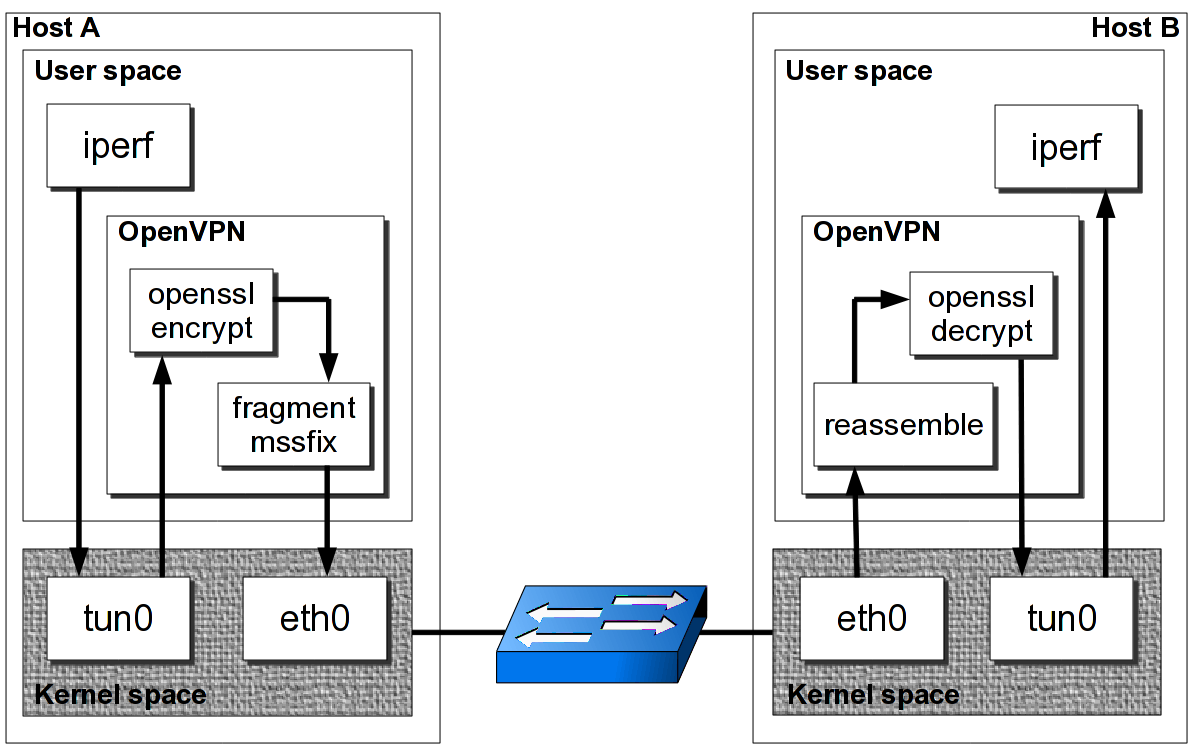
\includegraphics[width=\textwidth]{OpenVPN-packetflow}
\caption{OpenVPN packet flow}{it shows two hosts using \texttt{iperf} inside an OpenVPN tunnel. This figure comes from the OpenVPN documentation~\cite{openvpn-doc-workflow} and has inverted the encryption and fragmentation.}
\label{fig:openvpn-packet-flow}
\end{figure}

\noindent At this point, it is important to note that if the figure~\ref{fig:openvpn-packet-flow} shows a workflow in which the encryption taking place before the fragmentation, a quick look at the source code proves the opposite.
A sample of the said code has been writen down in the listing~\ref{list:openvpn-workflow}.


\lstset{language=c}
\begin{lstlisting}[caption={openvpn compress then encrypt -- sample from \texttt{forward.c}. It clearly shows that the order of operations in the packet workflow is compression, then fragmentation and finally encryption.}, label=list:openvpn-workflow, float]% The 'float' option makes the listing unbreakable.
/* Compress, fragment, encrypt and HMAC-sign an outgoing packet. */
void encrypt_sign (struct context *c, bool comp_frag)
{
	struct context_buffers *b = c->c2.buffers;
	const uint8_t *orig_buf = c->c2.buf.data;

	if (comp_frag){
	/* Compress the packet. */
		if (lzo_defined (&c->c2.lzo_compwork))
			lzo_compress (&c->c2.buf, b->lzo_compress_buf, &c->c2.lzo_compwork, &c->c2.frame);
	/* Fragment the packet. */
		if (c->c2.fragment)
			fragment_outgoing (c->c2.fragment, &c->c2.buf, &c->c2.frame_fragment);
	}

  /* Encrypt the packet and write an optional HMAC signature. */
	openvpn_encrypt (&c->c2.buf, b->encrypt_buf, &c->c2.crypto_options, &c->c2.frame);
}
\end{lstlisting}

An other way to look at this workflow is to completely isolate the OpenVPN part from both hosts, and exporting it to an independent device such as a router.
The hosts would be stripped off the virtual interface -- \texttt{tun0} would become physical, and would communicate normally over the internet, at least from their point of view.
All their communications would be routed by the router of their local area network, incomming on a physical \texttt{tun0} interface and outputed to the internet on the \texttt{eth0} interface.
Such implementation are used when an adminstrator wishes to secure a whole local area network without bloating each client with a VPN application.
In this case, there exist router firmware packages running OpenVPN, such as DD-WRT and OpenWRT.
Whatever the method used, the crucial point is that the VPN tunnel usage is transparent to the application.\newline{}

OpenVPN relies on a cryptographic library, OpenSSL in our case, for all the security operations: encryption, signature, certificate management, etc.

\noindent Note that if one wants to use the \texttt{none} cipher with a version of OpenVPN ealier than 2.3.7, he would have to update it using a community patch~\cite{openvpn-patch-none}.

\subsection{OpenSSH}
% Talk about the MAC=none patch
% connection using SSL/TLS, then AES, but without fragmentation (unlike openvpn)
OpenSSH relies on an external cryptographic library for all its security operations.
Up until the version 6.7 published in october 2014, it had to be compiled against OpenSSL.
However, after the infamous security vulnerability heartbleed in april 2014, the developpers took a step to move towards LibreSSL, a fork of OpenSSL managed by OpenBSD  developers.
Still, there is no official support for any other cryptographic library.

If OpenSSH does support most of OpenSSL ciphers by default, it takes some liberties such as disabling the CBC encryption mode and removing the support of no MAC during a transmission.

\noindent The first liberty is a laste\footnote{A vulnerability note as been issued by Carnegie Mellon University Computer Emergency Response Team in early 2009 (last revision)~\cite{CERT2009}, in response to a research of University of London~\cite{Albrecht:2009} presenting a plaintext-recovering attack against SSH when CBC mode is used, but the OpenSSH update took only place in october 2014.}.
Even if it is not recommended, the user can still enable this mode by explicitly configuring it in the \texttt{sshd\_config} options.

\noindent The second liberty has been taken to prevent the user to strip himself from data authenticity and integrity.
However, in the case of testing and benchmarking, leaving the MAC behind can be interresting, especially if it is not offloaded in hardware such as the encryption in our case.
In order to add this feature to OpenSSH, we wrote a patch to apply on OpenSSH 6.7, available in appendix~\ref{chap:openssh-patch}.




\subsection{OpenSSL}

Offers an high-level interface called EVP to be used by other applications.


It is to be noted that the present work uses an implementation with all the debug flags activated.
Figure~\ref{fig:openssl-speed-dbg-on-off} shows that if it does have an impact on the performance, it is minimal: in the worst case of the benchmark, the throughput drops only by 2.4\%.
Moreover, the benchmark maximizes this difference by doing only OpenSSL operations.
When OpenSSL will have to share the CPU with other applications, the loss will be even less noticeable.
\begin{figure}[ht]
\begin{tikzpicture}
\begin{axis}[
		title = {Openssl speed with debug on/off},
        width  = 0.85*\textwidth,
        height = 8cm,
        major x tick style = transparent,
        ybar,
        bar width=8pt,
        ymajorgrids = true,
        ylabel = {Throughput [$10^3$kB/s]},
        xlabel = {Packet size},
        ymin=0,
        symbolic x coords={16,64,256,1024,8192},
        xtick = data,
        scaled y ticks = false,%Disable the *10^4 exponent applied to all y axis markings.
        legend style={at={(0.5,-0.25)},	anchor=north,legend columns=2},
        enlarge x limits=0.1,
    ]
\addplot[style={MidnightBlue,fill=MidnightBlue,mark=none}]
	coordinates {(16,18400.60) (64,20750.61) (256,21507.33) (1024,21681.15) (8192,21725.18)};
	\label{aes-256-cbc-dbg-off}

\addplot[style={Aquamarine,fill=Aquamarine,mark=none}]
	coordinates {(16,19091.65) (64,20579.24) (256,21106.60) (1024,21216.26) (8192,21203.63)};
	\label{aes-256-cbc-dbg-on}

\addplot[style={ForestGreen,fill=ForestGreen,mark=none}]
	coordinates {(16,23882.41) (64,27781.80) (256,29285.63) (1024,29692.25) (8192,29807.96)};
	\label{aes-128-cbc-dbg-off}

\addplot[style={YellowGreen,fill=YellowGreen,mark=none}]
	coordinates {(16,23806.36) (64,27728.96) (256,29181.70) (1024,29573.46) (8192,29687.81)};
	\label{aes-128-cbc-dbg-on}

\legend{AES-256-CBC debug [off], AES-256-CBC debug [on], AES-128-CBC debug [off], AES-128-CBC debug [on]}
\end{axis}
\end{tikzpicture}
\caption{OpenSSL debugging benchmark}{Software benchmark of Openssl speed for AES mode CBC, with 128- and 256-bit keys, debugging flags (de)activated at compilation (\texttt{-fno-inline -g -marm}). The throughput difference ranges from 0.2\% and 2.4\% , and is more marked for larger keysize, as more debugging data needs to be generated.}
\label{fig:openssl-speed-dbg-on-off}
\end{figure}

% Talk about the assembly implementation, maybe show the difference in an appendice with the C implementation. Not /that/ interresting.


\subsection{Strongswan}
% TODO talk about IKE and SA management
Strongswan is a full implementation of IPSec relying on the kernel drivers for the networking part, on the crypto API for the cryptographic part, and on user space crypto libraries for the connection negociation.
An other popular implementation is ipsec-tools, but its development lags behind modern Linux and is not up-to-date with the 3.14 Linux kernel headers, making its cross-compilation painfull.
%Use strongswan 5.3.0
Strongswan as two advantages: it has a tremendous and exhaustive documentation, and its uer interface is straightforward.
Once configured, a simple \texttt{ipsec start \&\& ipsec up <connection>} on both sides is enough to create a ready to use VPN.

The figure~\ref{fig:ipsec-workflow} illustrates the workflow of Alice communicating with Bob via an IPSec ESP tunnel.
The XFRM, read ``transform", framework is implementing IPSec and handles the incomming and outgoing packets for established VPNs~\cite{rosen2014}.
Its name comes from the fact that the kernel transforms packet frames to incorporate IPSec security.
Depending on the configuration, XFRM uses the AH or ESP kernel module, which in turn calls the crypto API to encrypt and/or sign the IP packet.

We can also clearly see one of the main advantages of IPSec: it works in the kernel space.
Since it does not require a virtual network interface like OpenVPN, the only transfer between the user/kernel space happens when the former wishes to send a packet on the network, passing it to the later -- or \textit{vice versa} for incomming packets.

\begin{figure}[ht]
\Large
\resizebox{\linewidth}{!}{%
% Graphic for TeX using PGF
% Title: /home/para/documents/polytech2015/MA2/Master_thesis/master_thesis/ipsec-transfer.dia
% Creator: Dia v0.97.3
% CreationDate: Sat May 16 13:42:52 2015
% For: para
% \usepackage{tikz}
% The following commands are not supported in PSTricks at present
% We define them conditionally, so when they are implemented,
% this pgf file will use them.
\ifx\du\undefined
  \newlength{\du}
\fi
\setlength{\du}{15\unitlength}
\begin{tikzpicture}
\pgftransformxscale{1.000000}
\pgftransformyscale{-1.000000}
\definecolor{dialinecolor}{rgb}{0.000000, 0.000000, 0.000000}
\pgfsetstrokecolor{dialinecolor}
\definecolor{dialinecolor}{rgb}{1.000000, 1.000000, 1.000000}
\pgfsetfillcolor{dialinecolor}
\pgfsetlinewidth{0.050000\du}
\pgfsetdash{}{0pt}
\pgfsetdash{}{0pt}
\pgfsetmiterjoin
\definecolor{dialinecolor}{rgb}{1.000000, 1.000000, 1.000000}
\pgfsetfillcolor{dialinecolor}
\fill (6.600000\du,9.800000\du)--(6.600000\du,10.800000\du)--(14.400000\du,10.800000\du)--(14.400000\du,9.800000\du)--cycle;
\definecolor{dialinecolor}{rgb}{0.000000, 0.000000, 0.000000}
\pgfsetstrokecolor{dialinecolor}
\draw (6.600000\du,9.800000\du)--(6.600000\du,10.800000\du)--(14.400000\du,10.800000\du)--(14.400000\du,9.800000\du)--cycle;
\pgfsetlinewidth{0.050000\du}
\pgfsetdash{}{0pt}
\pgfsetdash{}{0pt}
\pgfsetmiterjoin
\definecolor{dialinecolor}{rgb}{1.000000, 1.000000, 1.000000}
\pgfsetfillcolor{dialinecolor}
\fill (6.600000\du,9.800000\du)--(6.600000\du,18.600000\du)--(14.400000\du,18.600000\du)--(14.400000\du,9.800000\du)--cycle;
\definecolor{dialinecolor}{rgb}{0.000000, 0.000000, 0.000000}
\pgfsetstrokecolor{dialinecolor}
\draw (6.600000\du,9.800000\du)--(6.600000\du,18.600000\du)--(14.400000\du,18.600000\du)--(14.400000\du,9.800000\du)--cycle;
% setfont left to latex
\definecolor{dialinecolor}{rgb}{0.000000, 0.000000, 0.000000}
\pgfsetstrokecolor{dialinecolor}
\node at (10.500000\du,10.416250\du){Alice};
\pgfsetlinewidth{0.050000\du}
\pgfsetdash{}{0pt}
\pgfsetdash{}{0pt}
\pgfsetmiterjoin
\definecolor{dialinecolor}{rgb}{1.000000, 1.000000, 1.000000}
\pgfsetfillcolor{dialinecolor}
\fill (18.600000\du,9.800000\du)--(18.600000\du,10.800000\du)--(26.400000\du,10.800000\du)--(26.400000\du,9.800000\du)--cycle;
\definecolor{dialinecolor}{rgb}{0.000000, 0.000000, 0.000000}
\pgfsetstrokecolor{dialinecolor}
\draw (18.600000\du,9.800000\du)--(18.600000\du,10.800000\du)--(26.400000\du,10.800000\du)--(26.400000\du,9.800000\du)--cycle;
\pgfsetlinewidth{0.050000\du}
\pgfsetdash{}{0pt}
\pgfsetdash{}{0pt}
\pgfsetmiterjoin
\definecolor{dialinecolor}{rgb}{1.000000, 1.000000, 1.000000}
\pgfsetfillcolor{dialinecolor}
\fill (18.600000\du,9.800000\du)--(18.600000\du,18.600000\du)--(26.400000\du,18.600000\du)--(26.400000\du,9.800000\du)--cycle;
\definecolor{dialinecolor}{rgb}{0.000000, 0.000000, 0.000000}
\pgfsetstrokecolor{dialinecolor}
\draw (18.600000\du,9.800000\du)--(18.600000\du,18.600000\du)--(26.400000\du,18.600000\du)--(26.400000\du,9.800000\du)--cycle;
% setfont left to latex
\definecolor{dialinecolor}{rgb}{0.000000, 0.000000, 0.000000}
\pgfsetstrokecolor{dialinecolor}
\node at (22.500000\du,10.411344\du){Bob};
\pgfsetlinewidth{0.050000\du}
\pgfsetdash{}{0pt}
\pgfsetdash{}{0pt}
\pgfsetmiterjoin
\definecolor{dialinecolor}{rgb}{1.000000, 1.000000, 1.000000}
\pgfsetfillcolor{dialinecolor}
\fill (7.000000\du,13.000000\du)--(7.000000\du,14.000000\du)--(9.400000\du,14.000000\du)--(9.400000\du,13.000000\du)--cycle;
\definecolor{dialinecolor}{rgb}{0.000000, 0.000000, 0.000000}
\pgfsetstrokecolor{dialinecolor}
\draw (7.000000\du,13.000000\du)--(7.000000\du,14.000000\du)--(9.400000\du,14.000000\du)--(9.400000\du,13.000000\du)--cycle;
\pgfsetlinewidth{0.050000\du}
\pgfsetdash{}{0pt}
\pgfsetdash{}{0pt}
\pgfsetmiterjoin
\definecolor{dialinecolor}{rgb}{0.905882, 0.905882, 0.905882}
\pgfsetfillcolor{dialinecolor}
\fill (7.000000\du,13.000000\du)--(7.000000\du,18.200000\du)--(14.000000\du,18.200000\du)--(14.000000\du,13.000000\du)--cycle;
\definecolor{dialinecolor}{rgb}{0.000000, 0.000000, 0.000000}
\pgfsetstrokecolor{dialinecolor}
\draw (7.000000\du,13.000000\du)--(7.000000\du,18.200000\du)--(14.000000\du,18.200000\du)--(14.000000\du,13.000000\du)--cycle;
\pgfsetlinewidth{0.000000\du}
\pgfsetdash{}{0pt}
\pgfsetdash{}{0pt}
\pgfsetmiterjoin
\definecolor{dialinecolor}{rgb}{1.000000, 1.000000, 1.000000}
\pgfsetfillcolor{dialinecolor}
\fill (7.000000\du,10.800000\du)--(7.000000\du,11.800000\du)--(9.000000\du,11.800000\du)--(9.000000\du,10.800000\du)--cycle;
\definecolor{dialinecolor}{rgb}{1.000000, 1.000000, 1.000000}
\pgfsetstrokecolor{dialinecolor}
\draw (7.000000\du,10.800000\du)--(7.000000\du,11.800000\du)--(9.000000\du,11.800000\du)--(9.000000\du,10.800000\du)--cycle;
\pgfsetlinewidth{0.050000\du}
\pgfsetdash{}{0pt}
\pgfsetdash{}{0pt}
\pgfsetmiterjoin
\definecolor{dialinecolor}{rgb}{1.000000, 1.000000, 1.000000}
\pgfsetfillcolor{dialinecolor}
\fill (7.000000\du,10.800000\du)--(7.000000\du,12.600000\du)--(14.000000\du,12.600000\du)--(14.000000\du,10.800000\du)--cycle;
\definecolor{dialinecolor}{rgb}{0.000000, 0.000000, 0.000000}
\pgfsetstrokecolor{dialinecolor}
\draw (7.000000\du,10.800000\du)--(7.000000\du,12.600000\du)--(14.000000\du,12.600000\du)--(14.000000\du,10.800000\du)--cycle;
% setfont left to latex
\definecolor{dialinecolor}{rgb}{0.000000, 0.000000, 0.000000}
\pgfsetstrokecolor{dialinecolor}
\node at (8.000000\du,11.416250\du){User};
% setfont left to latex
\definecolor{dialinecolor}{rgb}{0.000000, 0.000000, 0.000000}
\pgfsetstrokecolor{dialinecolor}
\node at (8.200000\du,13.616250\du){Kernel};
\pgfsetlinewidth{0.050000\du}
\pgfsetdash{}{0pt}
\pgfsetdash{}{0pt}
\pgfsetmiterjoin
\definecolor{dialinecolor}{rgb}{1.000000, 1.000000, 1.000000}
\pgfsetfillcolor{dialinecolor}
\fill (23.600000\du,13.000000\du)--(23.600000\du,14.000000\du)--(26.000000\du,14.000000\du)--(26.000000\du,13.000000\du)--cycle;
\definecolor{dialinecolor}{rgb}{0.000000, 0.000000, 0.000000}
\pgfsetstrokecolor{dialinecolor}
\draw (23.600000\du,13.000000\du)--(23.600000\du,14.000000\du)--(26.000000\du,14.000000\du)--(26.000000\du,13.000000\du)--cycle;
\pgfsetlinewidth{0.050000\du}
\pgfsetdash{}{0pt}
\pgfsetdash{}{0pt}
\pgfsetmiterjoin
\definecolor{dialinecolor}{rgb}{0.905882, 0.905882, 0.905882}
\pgfsetfillcolor{dialinecolor}
\fill (19.000000\du,13.000000\du)--(19.000000\du,18.200000\du)--(26.000000\du,18.200000\du)--(26.000000\du,13.000000\du)--cycle;
\definecolor{dialinecolor}{rgb}{0.000000, 0.000000, 0.000000}
\pgfsetstrokecolor{dialinecolor}
\draw (19.000000\du,13.000000\du)--(19.000000\du,18.200000\du)--(26.000000\du,18.200000\du)--(26.000000\du,13.000000\du)--cycle;
\pgfsetlinewidth{0.000000\du}
\pgfsetdash{}{0pt}
\pgfsetdash{}{0pt}
\pgfsetmiterjoin
\definecolor{dialinecolor}{rgb}{1.000000, 1.000000, 1.000000}
\pgfsetfillcolor{dialinecolor}
\fill (24.000000\du,10.800000\du)--(24.000000\du,11.800000\du)--(26.000000\du,11.800000\du)--(26.000000\du,10.800000\du)--cycle;
\definecolor{dialinecolor}{rgb}{1.000000, 1.000000, 1.000000}
\pgfsetstrokecolor{dialinecolor}
\draw (24.000000\du,10.800000\du)--(24.000000\du,11.800000\du)--(26.000000\du,11.800000\du)--(26.000000\du,10.800000\du)--cycle;
\pgfsetlinewidth{0.050000\du}
\pgfsetdash{}{0pt}
\pgfsetdash{}{0pt}
\pgfsetmiterjoin
\definecolor{dialinecolor}{rgb}{1.000000, 1.000000, 1.000000}
\pgfsetfillcolor{dialinecolor}
\fill (19.000000\du,10.800000\du)--(19.000000\du,12.600000\du)--(26.000000\du,12.600000\du)--(26.000000\du,10.800000\du)--cycle;
\definecolor{dialinecolor}{rgb}{0.000000, 0.000000, 0.000000}
\pgfsetstrokecolor{dialinecolor}
\draw (19.000000\du,10.800000\du)--(19.000000\du,12.600000\du)--(26.000000\du,12.600000\du)--(26.000000\du,10.800000\du)--cycle;
% setfont left to latex
\definecolor{dialinecolor}{rgb}{0.000000, 0.000000, 0.000000}
\pgfsetstrokecolor{dialinecolor}
\node at (25.000000\du,11.416250\du){User};
% setfont left to latex
\definecolor{dialinecolor}{rgb}{0.000000, 0.000000, 0.000000}
\pgfsetstrokecolor{dialinecolor}
\node at (24.800000\du,13.616250\du){Kernel};
\pgfsetlinewidth{0.020000\du}
\pgfsetdash{}{0pt}
\pgfsetdash{}{0pt}
\pgfsetbuttcap
\pgfsetmiterjoin
\pgfsetlinewidth{0.000200\du}
\pgfsetbuttcap
\pgfsetmiterjoin
\pgfsetdash{}{0pt}
\definecolor{dialinecolor}{rgb}{0.000000, 0.588235, 0.831373}
\pgfsetfillcolor{dialinecolor}
\pgfpathmoveto{\pgfpoint{14.600000\du}{14.000632\du}}
\pgfpathlineto{\pgfpoint{14.600000\du}{14.731085\du}}
\pgfpathlineto{\pgfpoint{17.488279\du}{14.731085\du}}
\pgfpathlineto{\pgfpoint{17.488279\du}{14.000632\du}}
\pgfpathlineto{\pgfpoint{14.600000\du}{14.000632\du}}
\pgfusepath{fill}
\pgfsetbuttcap
\pgfsetmiterjoin
\pgfsetdash{}{0pt}
\definecolor{dialinecolor}{rgb}{0.666667, 0.901961, 1.000000}
\pgfsetstrokecolor{dialinecolor}
\pgfpathmoveto{\pgfpoint{14.600000\du}{14.000632\du}}
\pgfpathlineto{\pgfpoint{14.600000\du}{14.731085\du}}
\pgfpathlineto{\pgfpoint{17.488279\du}{14.731085\du}}
\pgfpathlineto{\pgfpoint{17.488279\du}{14.000632\du}}
\pgfpathlineto{\pgfpoint{14.600000\du}{14.000632\du}}
\pgfusepath{stroke}
\pgfsetbuttcap
\pgfsetmiterjoin
\pgfsetdash{}{0pt}
\definecolor{dialinecolor}{rgb}{0.000000, 0.352941, 0.501961}
\pgfsetfillcolor{dialinecolor}
\pgfpathmoveto{\pgfpoint{17.488279\du}{14.000632\du}}
\pgfpathlineto{\pgfpoint{18.381785\du}{13.140000\du}}
\pgfpathlineto{\pgfpoint{18.381785\du}{13.871110\du}}
\pgfpathlineto{\pgfpoint{17.488279\du}{14.731085\du}}
\pgfpathlineto{\pgfpoint{17.488279\du}{14.000632\du}}
\pgfusepath{fill}
\pgfsetbuttcap
\pgfsetmiterjoin
\pgfsetdash{}{0pt}
\definecolor{dialinecolor}{rgb}{0.666667, 0.901961, 1.000000}
\pgfsetstrokecolor{dialinecolor}
\pgfpathmoveto{\pgfpoint{17.488279\du}{14.000632\du}}
\pgfpathlineto{\pgfpoint{18.381785\du}{13.140000\du}}
\pgfpathlineto{\pgfpoint{18.381785\du}{13.871110\du}}
\pgfpathlineto{\pgfpoint{17.488279\du}{14.731085\du}}
\pgfpathlineto{\pgfpoint{17.488279\du}{14.000632\du}}
\pgfusepath{stroke}
\pgfsetbuttcap
\pgfsetmiterjoin
\pgfsetdash{}{0pt}
\definecolor{dialinecolor}{rgb}{0.000000, 0.705882, 1.000000}
\pgfsetfillcolor{dialinecolor}
\pgfpathmoveto{\pgfpoint{17.488279\du}{14.000632\du}}
\pgfpathlineto{\pgfpoint{18.381785\du}{13.140000\du}}
\pgfpathlineto{\pgfpoint{15.492848\du}{13.140000\du}}
\pgfpathlineto{\pgfpoint{14.600000\du}{14.000632\du}}
\pgfpathlineto{\pgfpoint{17.488279\du}{14.000632\du}}
\pgfusepath{fill}
\pgfsetbuttcap
\pgfsetmiterjoin
\pgfsetdash{}{0pt}
\definecolor{dialinecolor}{rgb}{0.666667, 0.901961, 1.000000}
\pgfsetstrokecolor{dialinecolor}
\pgfpathmoveto{\pgfpoint{17.488279\du}{14.000632\du}}
\pgfpathlineto{\pgfpoint{18.381785\du}{13.140000\du}}
\pgfpathlineto{\pgfpoint{15.492848\du}{13.140000\du}}
\pgfpathlineto{\pgfpoint{14.600000\du}{14.000632\du}}
\pgfpathlineto{\pgfpoint{17.488279\du}{14.000632\du}}
\pgfusepath{stroke}
\pgfsetbuttcap
\pgfsetmiterjoin
\pgfsetdash{}{0pt}
\definecolor{dialinecolor}{rgb}{0.000000, 0.000000, 0.000000}
\pgfsetfillcolor{dialinecolor}
\pgfpathmoveto{\pgfpoint{15.544789\du}{13.452300\du}}
\pgfpathlineto{\pgfpoint{15.388968\du}{13.608778\du}}
\pgfpathlineto{\pgfpoint{17.122067\du}{13.608778\du}}
\pgfpathlineto{\pgfpoint{16.989257\du}{13.739615\du}}
\pgfpathlineto{\pgfpoint{17.724970\du}{13.556838\du}}
\pgfpathlineto{\pgfpoint{17.358100\du}{13.374060\du}}
\pgfpathlineto{\pgfpoint{17.278545\du}{13.452300\du}}
\pgfpathlineto{\pgfpoint{15.544789\du}{13.452300\du}}
\pgfusepath{fill}
\pgfsetbuttcap
\pgfsetmiterjoin
\pgfsetdash{}{0pt}
\definecolor{dialinecolor}{rgb}{1.000000, 1.000000, 1.000000}
\pgfsetfillcolor{dialinecolor}
\pgfpathmoveto{\pgfpoint{15.571088\du}{13.478599\du}}
\pgfpathlineto{\pgfpoint{15.413294\du}{13.608778\du}}
\pgfpathlineto{\pgfpoint{17.147051\du}{13.608778\du}}
\pgfpathlineto{\pgfpoint{17.015556\du}{13.739615\du}}
\pgfpathlineto{\pgfpoint{17.724970\du}{13.583794\du}}
\pgfpathlineto{\pgfpoint{17.383084\du}{13.401017\du}}
\pgfpathlineto{\pgfpoint{17.278545\du}{13.478599\du}}
\pgfpathlineto{\pgfpoint{15.571088\du}{13.478599\du}}
\pgfusepath{fill}
\pgfsetlinewidth{0.020000\du}
\pgfsetdash{}{0pt}
\pgfsetdash{}{0pt}
\pgfsetmiterjoin
\definecolor{dialinecolor}{rgb}{1.000000, 1.000000, 1.000000}
\pgfsetfillcolor{dialinecolor}
\fill (11.000000\du,11.500000\du)--(11.000000\du,12.000000\du)--(13.000000\du,12.000000\du)--(13.000000\du,11.500000\du)--cycle;
\definecolor{dialinecolor}{rgb}{0.000000, 0.000000, 0.000000}
\pgfsetstrokecolor{dialinecolor}
\draw (11.000000\du,11.500000\du)--(11.000000\du,12.000000\du)--(13.000000\du,12.000000\du)--(13.000000\du,11.500000\du)--cycle;
% setfont left to latex
\definecolor{dialinecolor}{rgb}{0.000000, 0.000000, 0.000000}
\pgfsetstrokecolor{dialinecolor}
\node at (12.000000\du,11.750000\du){ping};
\pgfsetlinewidth{0.020000\du}
\pgfsetdash{}{0pt}
\pgfsetdash{}{0pt}
\pgfsetmiterjoin
\definecolor{dialinecolor}{rgb}{1.000000, 1.000000, 1.000000}
\pgfsetfillcolor{dialinecolor}
\fill (11.000000\du,13.500000\du)--(11.000000\du,14.500000\du)--(13.000000\du,14.500000\du)--(13.000000\du,13.500000\du)--cycle;
\definecolor{dialinecolor}{rgb}{0.000000, 0.000000, 0.000000}
\pgfsetstrokecolor{dialinecolor}
\draw (11.000000\du,13.500000\du)--(11.000000\du,14.500000\du)--(13.000000\du,14.500000\du)--(13.000000\du,13.500000\du)--cycle;
% setfont left to latex
\definecolor{dialinecolor}{rgb}{0.000000, 0.000000, 0.000000}
\pgfsetstrokecolor{dialinecolor}
\node at (12.000000\du,14.000000\du){XFRM};
\pgfsetlinewidth{0.020000\du}
\pgfsetdash{}{0pt}
\pgfsetdash{}{0pt}
\pgfsetmiterjoin
\definecolor{dialinecolor}{rgb}{1.000000, 1.000000, 1.000000}
\pgfsetfillcolor{dialinecolor}
\fill (11.300000\du,16.000000\du)--(11.300000\du,16.500000\du)--(12.700000\du,16.500000\du)--(12.700000\du,16.000000\du)--cycle;
\definecolor{dialinecolor}{rgb}{0.000000, 0.000000, 0.000000}
\pgfsetstrokecolor{dialinecolor}
\draw (11.300000\du,16.000000\du)--(11.300000\du,16.500000\du)--(12.700000\du,16.500000\du)--(12.700000\du,16.000000\du)--cycle;
% setfont left to latex
\definecolor{dialinecolor}{rgb}{0.000000, 0.000000, 0.000000}
\pgfsetstrokecolor{dialinecolor}
\node at (12.000000\du,16.250000\du){ESP};
\pgfsetlinewidth{0.020000\du}
\pgfsetdash{}{0pt}
\pgfsetdash{}{0pt}
\pgfsetmiterjoin
\definecolor{dialinecolor}{rgb}{1.000000, 1.000000, 1.000000}
\pgfsetfillcolor{dialinecolor}
\fill (7.600000\du,16.000000\du)--(7.600000\du,16.500000\du)--(9.900000\du,16.500000\du)--(9.900000\du,16.000000\du)--cycle;
\definecolor{dialinecolor}{rgb}{0.000000, 0.000000, 0.000000}
\pgfsetstrokecolor{dialinecolor}
\draw (7.600000\du,16.000000\du)--(7.600000\du,16.500000\du)--(9.900000\du,16.500000\du)--(9.900000\du,16.000000\du)--cycle;
% setfont left to latex
\definecolor{dialinecolor}{rgb}{0.000000, 0.000000, 0.000000}
\pgfsetstrokecolor{dialinecolor}
\node at (8.750000\du,16.250000\du){Crypto API};
\pgfsetlinewidth{0.020000\du}
\pgfsetdash{}{0pt}
\pgfsetdash{}{0pt}
\pgfsetmiterjoin
\definecolor{dialinecolor}{rgb}{1.000000, 1.000000, 1.000000}
\pgfsetfillcolor{dialinecolor}
\fill (7.500000\du,17.100000\du)--(7.500000\du,17.600000\du)--(8.700000\du,17.600000\du)--(8.700000\du,17.100000\du)--cycle;
\definecolor{dialinecolor}{rgb}{0.000000, 0.000000, 0.000000}
\pgfsetstrokecolor{dialinecolor}
\draw (7.500000\du,17.100000\du)--(7.500000\du,17.600000\du)--(8.700000\du,17.600000\du)--(8.700000\du,17.100000\du)--cycle;
% setfont left to latex
\definecolor{dialinecolor}{rgb}{0.000000, 0.000000, 0.000000}
\pgfsetstrokecolor{dialinecolor}
\node at (8.100000\du,17.350000\du){S/W};
\pgfsetlinewidth{0.020000\du}
\pgfsetdash{}{0pt}
\pgfsetdash{}{0pt}
\pgfsetmiterjoin
\definecolor{dialinecolor}{rgb}{1.000000, 1.000000, 1.000000}
\pgfsetfillcolor{dialinecolor}
\fill (8.800000\du,17.100000\du)--(8.800000\du,17.600000\du)--(10.000000\du,17.600000\du)--(10.000000\du,17.100000\du)--cycle;
\definecolor{dialinecolor}{rgb}{0.000000, 0.000000, 0.000000}
\pgfsetstrokecolor{dialinecolor}
\draw (8.800000\du,17.100000\du)--(8.800000\du,17.600000\du)--(10.000000\du,17.600000\du)--(10.000000\du,17.100000\du)--cycle;
% setfont left to latex
\definecolor{dialinecolor}{rgb}{0.000000, 0.000000, 0.000000}
\pgfsetstrokecolor{dialinecolor}
\node at (9.400000\du,17.350000\du){H/W};
\pgfsetlinewidth{0.020000\du}
\pgfsetdash{}{0pt}
\pgfsetdash{}{0pt}
\pgfsetbuttcap
{
\definecolor{dialinecolor}{rgb}{0.000000, 0.000000, 0.000000}
\pgfsetfillcolor{dialinecolor}
% was here!!!
\pgfsetarrowsend{stealth}
\definecolor{dialinecolor}{rgb}{0.000000, 0.000000, 0.000000}
\pgfsetstrokecolor{dialinecolor}
\draw (12.000000\du,14.500000\du)--(12.000000\du,16.000000\du);
}
\pgfsetlinewidth{0.020000\du}
\pgfsetdash{}{0pt}
\pgfsetdash{}{0pt}
\pgfsetbuttcap
{
\definecolor{dialinecolor}{rgb}{0.000000, 0.000000, 0.000000}
\pgfsetfillcolor{dialinecolor}
% was here!!!
\pgfsetarrowsend{stealth}
\definecolor{dialinecolor}{rgb}{0.000000, 0.000000, 0.000000}
\pgfsetstrokecolor{dialinecolor}
\draw (11.300000\du,16.250000\du)--(9.900000\du,16.250000\du);
}
\pgfsetlinewidth{0.020000\du}
\pgfsetdash{}{0pt}
\pgfsetdash{}{0pt}
\pgfsetbuttcap
{
\definecolor{dialinecolor}{rgb}{0.000000, 0.000000, 0.000000}
\pgfsetfillcolor{dialinecolor}
% was here!!!
\pgfsetarrowsend{stealth}
\definecolor{dialinecolor}{rgb}{0.000000, 0.000000, 0.000000}
\pgfsetstrokecolor{dialinecolor}
\draw (8.750000\du,16.500000\du)--(8.100000\du,17.100000\du);
}
\pgfsetlinewidth{0.020000\du}
\pgfsetdash{}{0pt}
\pgfsetdash{}{0pt}
\pgfsetbuttcap
{
\definecolor{dialinecolor}{rgb}{0.000000, 0.000000, 0.000000}
\pgfsetfillcolor{dialinecolor}
% was here!!!
\pgfsetarrowsend{stealth}
\definecolor{dialinecolor}{rgb}{0.000000, 0.000000, 0.000000}
\pgfsetstrokecolor{dialinecolor}
\draw (8.750000\du,16.500000\du)--(9.400000\du,17.100000\du);
}
\pgfsetlinewidth{0.020000\du}
\pgfsetdash{}{0pt}
\pgfsetdash{}{0pt}
\pgfsetbuttcap
{
\definecolor{dialinecolor}{rgb}{0.000000, 0.000000, 0.000000}
\pgfsetfillcolor{dialinecolor}
% was here!!!
\pgfsetarrowsend{stealth}
\definecolor{dialinecolor}{rgb}{0.000000, 0.000000, 0.000000}
\pgfsetstrokecolor{dialinecolor}
\draw (13.000000\du,14.000000\du)--(14.600000\du,14.000632\du);
}
\pgfsetlinewidth{0.020000\du}
\pgfsetdash{}{0pt}
\pgfsetdash{}{0pt}
\pgfsetbuttcap
{
\definecolor{dialinecolor}{rgb}{0.000000, 0.000000, 0.000000}
\pgfsetfillcolor{dialinecolor}
% was here!!!
\pgfsetarrowsend{stealth}
\definecolor{dialinecolor}{rgb}{0.000000, 0.000000, 0.000000}
\pgfsetstrokecolor{dialinecolor}
\draw (12.000000\du,12.000000\du)--(12.000000\du,13.500000\du);
}
\pgfsetlinewidth{0.020000\du}
\pgfsetdash{}{0pt}
\pgfsetdash{}{0pt}
\pgfsetmiterjoin
\pgfsetbuttcap
{
\definecolor{dialinecolor}{rgb}{0.000000, 0.000000, 0.000000}
\pgfsetfillcolor{dialinecolor}
% was here!!!
\pgfsetarrowsend{stealth}
{\pgfsetcornersarced{\pgfpoint{0.000000\du}{0.000000\du}}\definecolor{dialinecolor}{rgb}{0.000000, 0.000000, 0.000000}
\pgfsetstrokecolor{dialinecolor}
\draw (12.000000\du,16.500000\du)--(12.000000\du,17.000000\du)--(13.000000\du,17.000000\du)--(13.000000\du,14.500000\du);
}}
\pgfsetlinewidth{0.020000\du}
\pgfsetdash{}{0pt}
\pgfsetdash{}{0pt}
\pgfsetmiterjoin
\definecolor{dialinecolor}{rgb}{1.000000, 1.000000, 1.000000}
\pgfsetfillcolor{dialinecolor}
\fill (20.000000\du,11.500000\du)--(20.000000\du,12.000000\du)--(22.000000\du,12.000000\du)--(22.000000\du,11.500000\du)--cycle;
\definecolor{dialinecolor}{rgb}{0.000000, 0.000000, 0.000000}
\pgfsetstrokecolor{dialinecolor}
\draw (20.000000\du,11.500000\du)--(20.000000\du,12.000000\du)--(22.000000\du,12.000000\du)--(22.000000\du,11.500000\du)--cycle;
% setfont left to latex
\definecolor{dialinecolor}{rgb}{0.000000, 0.000000, 0.000000}
\pgfsetstrokecolor{dialinecolor}
\node at (21.000000\du,11.750000\du){ping};
\pgfsetlinewidth{0.020000\du}
\pgfsetdash{}{0pt}
\pgfsetdash{}{0pt}
\pgfsetmiterjoin
\definecolor{dialinecolor}{rgb}{1.000000, 1.000000, 1.000000}
\pgfsetfillcolor{dialinecolor}
\fill (20.000000\du,13.500000\du)--(20.000000\du,14.500000\du)--(22.000000\du,14.500000\du)--(22.000000\du,13.500000\du)--cycle;
\definecolor{dialinecolor}{rgb}{0.000000, 0.000000, 0.000000}
\pgfsetstrokecolor{dialinecolor}
\draw (20.000000\du,13.500000\du)--(20.000000\du,14.500000\du)--(22.000000\du,14.500000\du)--(22.000000\du,13.500000\du)--cycle;
% setfont left to latex
\definecolor{dialinecolor}{rgb}{0.000000, 0.000000, 0.000000}
\pgfsetstrokecolor{dialinecolor}
\node at (21.000000\du,14.000000\du){XFRM};
\pgfsetlinewidth{0.020000\du}
\pgfsetdash{}{0pt}
\pgfsetdash{}{0pt}
\pgfsetmiterjoin
\definecolor{dialinecolor}{rgb}{1.000000, 1.000000, 1.000000}
\pgfsetfillcolor{dialinecolor}
\fill (20.300000\du,16.000000\du)--(20.300000\du,16.500000\du)--(21.700000\du,16.500000\du)--(21.700000\du,16.000000\du)--cycle;
\definecolor{dialinecolor}{rgb}{0.000000, 0.000000, 0.000000}
\pgfsetstrokecolor{dialinecolor}
\draw (20.300000\du,16.000000\du)--(20.300000\du,16.500000\du)--(21.700000\du,16.500000\du)--(21.700000\du,16.000000\du)--cycle;
% setfont left to latex
\definecolor{dialinecolor}{rgb}{0.000000, 0.000000, 0.000000}
\pgfsetstrokecolor{dialinecolor}
\node at (21.000000\du,16.250000\du){ESP};
\pgfsetlinewidth{0.020000\du}
\pgfsetdash{}{0pt}
\pgfsetdash{}{0pt}
\pgfsetmiterjoin
\definecolor{dialinecolor}{rgb}{1.000000, 1.000000, 1.000000}
\pgfsetfillcolor{dialinecolor}
\fill (23.100000\du,16.000000\du)--(23.100000\du,16.500000\du)--(25.400000\du,16.500000\du)--(25.400000\du,16.000000\du)--cycle;
\definecolor{dialinecolor}{rgb}{0.000000, 0.000000, 0.000000}
\pgfsetstrokecolor{dialinecolor}
\draw (23.100000\du,16.000000\du)--(23.100000\du,16.500000\du)--(25.400000\du,16.500000\du)--(25.400000\du,16.000000\du)--cycle;
% setfont left to latex
\definecolor{dialinecolor}{rgb}{0.000000, 0.000000, 0.000000}
\pgfsetstrokecolor{dialinecolor}
\node at (24.250000\du,16.250000\du){Crypto API};
\pgfsetlinewidth{0.020000\du}
\pgfsetdash{}{0pt}
\pgfsetdash{}{0pt}
\pgfsetmiterjoin
\definecolor{dialinecolor}{rgb}{1.000000, 1.000000, 1.000000}
\pgfsetfillcolor{dialinecolor}
\fill (23.000000\du,17.100000\du)--(23.000000\du,17.600000\du)--(24.200000\du,17.600000\du)--(24.200000\du,17.100000\du)--cycle;
\definecolor{dialinecolor}{rgb}{0.000000, 0.000000, 0.000000}
\pgfsetstrokecolor{dialinecolor}
\draw (23.000000\du,17.100000\du)--(23.000000\du,17.600000\du)--(24.200000\du,17.600000\du)--(24.200000\du,17.100000\du)--cycle;
% setfont left to latex
\definecolor{dialinecolor}{rgb}{0.000000, 0.000000, 0.000000}
\pgfsetstrokecolor{dialinecolor}
\node at (23.600000\du,17.350000\du){S/W};
\pgfsetlinewidth{0.020000\du}
\pgfsetdash{}{0pt}
\pgfsetdash{}{0pt}
\pgfsetmiterjoin
\definecolor{dialinecolor}{rgb}{1.000000, 1.000000, 1.000000}
\pgfsetfillcolor{dialinecolor}
\fill (24.300000\du,17.100000\du)--(24.300000\du,17.600000\du)--(25.500000\du,17.600000\du)--(25.500000\du,17.100000\du)--cycle;
\definecolor{dialinecolor}{rgb}{0.000000, 0.000000, 0.000000}
\pgfsetstrokecolor{dialinecolor}
\draw (24.300000\du,17.100000\du)--(24.300000\du,17.600000\du)--(25.500000\du,17.600000\du)--(25.500000\du,17.100000\du)--cycle;
% setfont left to latex
\definecolor{dialinecolor}{rgb}{0.000000, 0.000000, 0.000000}
\pgfsetstrokecolor{dialinecolor}
\node at (24.900000\du,17.350000\du){H/W};
\pgfsetlinewidth{0.020000\du}
\pgfsetdash{}{0pt}
\pgfsetdash{}{0pt}
\pgfsetbuttcap
{
\definecolor{dialinecolor}{rgb}{0.000000, 0.000000, 0.000000}
\pgfsetfillcolor{dialinecolor}
% was here!!!
\pgfsetarrowsend{stealth}
\definecolor{dialinecolor}{rgb}{0.000000, 0.000000, 0.000000}
\pgfsetstrokecolor{dialinecolor}
\draw (21.000000\du,14.500000\du)--(21.000000\du,16.000000\du);
}
\pgfsetlinewidth{0.020000\du}
\pgfsetdash{}{0pt}
\pgfsetdash{}{0pt}
\pgfsetbuttcap
{
\definecolor{dialinecolor}{rgb}{0.000000, 0.000000, 0.000000}
\pgfsetfillcolor{dialinecolor}
% was here!!!
\pgfsetarrowsend{stealth}
\definecolor{dialinecolor}{rgb}{0.000000, 0.000000, 0.000000}
\pgfsetstrokecolor{dialinecolor}
\draw (21.700000\du,16.250000\du)--(23.100000\du,16.250000\du);
}
\pgfsetlinewidth{0.020000\du}
\pgfsetdash{}{0pt}
\pgfsetdash{}{0pt}
\pgfsetbuttcap
{
\definecolor{dialinecolor}{rgb}{0.000000, 0.000000, 0.000000}
\pgfsetfillcolor{dialinecolor}
% was here!!!
\pgfsetarrowsend{stealth}
\definecolor{dialinecolor}{rgb}{0.000000, 0.000000, 0.000000}
\pgfsetstrokecolor{dialinecolor}
\draw (24.250000\du,16.500000\du)--(23.600000\du,17.100000\du);
}
\pgfsetlinewidth{0.020000\du}
\pgfsetdash{}{0pt}
\pgfsetdash{}{0pt}
\pgfsetbuttcap
{
\definecolor{dialinecolor}{rgb}{0.000000, 0.000000, 0.000000}
\pgfsetfillcolor{dialinecolor}
% was here!!!
\pgfsetarrowsend{stealth}
\definecolor{dialinecolor}{rgb}{0.000000, 0.000000, 0.000000}
\pgfsetstrokecolor{dialinecolor}
\draw (24.250000\du,16.500000\du)--(24.900000\du,17.100000\du);
}
\pgfsetlinewidth{0.020000\du}
\pgfsetdash{}{0pt}
\pgfsetdash{}{0pt}
\pgfsetbuttcap
{
\definecolor{dialinecolor}{rgb}{0.000000, 0.000000, 0.000000}
\pgfsetfillcolor{dialinecolor}
% was here!!!
\pgfsetarrowsend{stealth}
\definecolor{dialinecolor}{rgb}{0.000000, 0.000000, 0.000000}
\pgfsetstrokecolor{dialinecolor}
\draw (18.381785\du,13.871110\du)--(19.980000\du,13.870000\du);
}
\pgfsetlinewidth{0.020000\du}
\pgfsetdash{}{0pt}
\pgfsetdash{}{0pt}
\pgfsetbuttcap
{
\definecolor{dialinecolor}{rgb}{0.000000, 0.000000, 0.000000}
\pgfsetfillcolor{dialinecolor}
% was here!!!
\pgfsetarrowsend{stealth}
\definecolor{dialinecolor}{rgb}{0.000000, 0.000000, 0.000000}
\pgfsetstrokecolor{dialinecolor}
\draw (21.000000\du,12.000000\du)--(21.000000\du,13.500000\du);
}
\pgfsetlinewidth{0.020000\du}
\pgfsetdash{}{0pt}
\pgfsetdash{}{0pt}
\pgfsetmiterjoin
\pgfsetbuttcap
{
\definecolor{dialinecolor}{rgb}{0.000000, 0.000000, 0.000000}
\pgfsetfillcolor{dialinecolor}
% was here!!!
\pgfsetarrowsend{stealth}
{\pgfsetcornersarced{\pgfpoint{0.000000\du}{0.000000\du}}\definecolor{dialinecolor}{rgb}{0.000000, 0.000000, 0.000000}
\pgfsetstrokecolor{dialinecolor}
\draw (21.000000\du,16.500000\du)--(21.000000\du,16.800000\du)--(20.000000\du,16.800000\du)--(20.000000\du,14.500000\du);
}}
\end{tikzpicture}

}
\caption{IPSec user/kernel space workflow, using \texttt{ping} as a test case.}{}
\label{fig:ipsec-workflow}
\end{figure}


\subsection{Linux drivers}
% Mention the fact that we use the assembly implementation of AES, not the generic C one.
% Need an lsmod here.
Several kernel modules are needed to implement the various cryptographic algorithm in software.
The GCM alone needs five different modules, and IPSec three others.
The following description addresses all the kernel modules required to run all the use cases presented in this work.


\begin{description}
	\item[\texttt{aes\_arm}] Assembly implementation of AES. This version is optimized to use the ARMv7 instruction set.
	\item[\texttt{sha256-generic}] C implementation of SHA-256.
	\item[\texttt{gfmult128}] Multiplication in $GF(2^128)$, needed by the GCM mode.
	\item[\texttt{ghash}] GHASH function needed by the authentication of the GCM mode.
	\item[\texttt{seqiv}] Sequence IV number generator, needed by the CTR and GCM modes.
	\item[\texttt{cbc}] C based CBC mode.
	\item[\texttt{gcm}] C base GCM mode.
	\item[\texttt{crypto\_null}] Null cipher. This basically does nothing on the plaintext, but it is still needed to propose the interface in the kernel.
	\item[\texttt{tun}] TUN/TAP network device, needed by OpenVPN.
	\item[\texttt{xfrm\_user}] XFRM operations.
	\item[\texttt{esp4}] IPv4 ESP implementation. The AH counterparty is also available in the \texttt{ah4} module.
	\item[\texttt{ipcomp}] IP compression module. Needed by IPSec if the option is activated in the configuration.
	\item[\texttt{cryptodev}] Creates \texttt{/dev/crypto}, giving access to the crypto API in the user space.
	\item[\texttt{uio}] User-space I/O driver, allowing to access the hardware memory from the user space, needed by our implementation of the BA414E driver.
\end{description}

\section{Offload}

The table~\ref{tab:ip-ciphers} summarizes the ciphers supported by the two Barco Silex' IPs used in this work.

\begin{table}[ht]
\begin{tabular}{|l|c|}\hline
IP & Ciphers \\ \hline
BA414E & RSA, DH, DSA, EC \\ 
BA411E & AES modes CBC, CTR, GCM, CCM, CFB, OFB, CTS, ECB \\ \hline
\end{tabular}
\caption{Summary of the ciphers supported by two of Barco Silex' IPs.}{}
\label{tab:ip-ciphers}
\end{table}

\subsection{BA411E Driver}
Takes the rightern path, which is the cleanest because the most versatile.
By pluging the driver into the crypto API, we offer a standard kernel interface that can be used by any other kernel driver, such as the ESP driver, or user-space application via the cryptodev driver and OpenSSL engine.

However, at the current state of development, the user-space and the kernel applications do not share the same driver.
The former is using an IRQ-based driver, whilst the latter is actively polling the hardware.
The reason why the IRQ-based driver can not be used by kernel-space application is because the current implementation uses sleep methods that, when called on other kernel drivers, put the kernel in panic mode and require the system to reboot.
An alternative is under development and is further discussed in the last part of this work, in section~\ref{sec:future-work}.

Be it IRQ or polling, the inner workings are the same and follow the exact same canvas as the default software implementation the different AES modes.


\subsection{BA414E Driver and Silex engine}
At the moment of development, there is no asymetric cryptography interface in the crypto API\footnote{A request for comment patch as been submitted to the Linux kernel mailing list~\cite{crypto-api-pk-encryption} in late April 2015, proposing a standard interface for public key encryption in the crypto API.}.
The BA414E can thus not be accessed using the same path as the BA411E and a user-space driver will be needed, that is the leftern path of figure~\ref{fig:os-path-generic-b}.
As presented in section~\ref{sec:theory-driver}, we will need to rely on an UIO driver to access the device from the user space.%=> How we will study the problematic, what tool are we going to use to make it clear?

\chapter{Test protocol}\label{chap:test-protocol}
This chapter presents the platform on which the tests will be undertaken, as well as the tests themselves.



\section{Experimental setup}
The experimental environment is built around a standard x86 host and an ARM Cortex-A9 alongside an Altera Cyclone V FPGA as the target.
Both are linked toghether through a network capped by 100Mbps switches.
Both stations have gigabits ethernet interface and could hence be directly connected to each other, but in that case the communication would be limited by the I/O transfers of the storage units -- a hard drive disk in one case, an micro-SD card in the second -- on which we can not depend to set a constant throughput limitation, as it is highly influenced by the data block size and general health of the support.


\subsection{x86 host}
The desktop host runs on Windows 7 Professional 64-bit, but a virtual machine using a Linux distribution is used for the developement and testings.

\begin{framed}
\begin{description}
	\item[OS] Ubuntu 12.04 LTS, kernel 3.16
	\item[CPU] Intel Core-i5 M560, 2.67GHz (two logical core out of four)
	\item[RAM] 1GB DDR3
\end{description}
\end{framed}

\subsection{EBV Socrates board}
The board if based on the SocFPGA from Altera: a combination of ARM cores and Altera Cyclone V FPGA.

\begin{framed}
\begin{description}
	\item[OS] Yocto project, kernel 3.14
	\item[CPU] Dual core ARM Cortex-A9, 800MHz
	\item[RAM] 1GB DDR3
	\item[FPGA] Altera Cyclone V
\end{description}
\end{framed}

\subsection{ARM DS-5 Streamline}
Streamline is a toolsuite included in ARM Development Studio.
By installing a kernel module and running a daemon on the board, it can fetch a huge amount of data without over-loading the system.
This tool is able to gather information on the CPU utilisation, the amount of context switches, of interrupts, of memory used, and much more.
If the applications, libraries and kernel modules have been compiled with the required debugging options, it can also build the call path of a run, giving extensive statistics on the most ressource-hungry functions.

If it has close to no impact on the performance of the board, the same does not go for the hosting machine.
A serious drawback is his memory consumption that, when combined with the ressources used by the virtual machine, bring the hosting machine to its knees.

\noindent The user should also be aware that if Streamline if a very powerfull and versatile tool, it is not reliable at very high resolution.
The data should not be analyzed in windows smaller than a millisecond.

\section{Test cases}
The aim of this work is to test the implementations under realistic situations.
To reach this goal, three test cases will be used:
\begin{itemize}
	\item Lots of connections without fetching any data.
	\item Latency of the connection. This test can also illustrate the transfer of small amount of data.
	\item Large file transfer on an established connection.
\end{itemize}

Each of those tests will go from a raw run, without any encryption nor authentication serving as a comparison ground, gradually increasing security up to a complete encryption/authentication scheme.

The table~\ref{tab:software-version} summarizes the softwares used and tjeir respective version.

\begin{table}
\center
\begin{tabular}{|l|l|} \hline
OpenVPN & 2.3.6 \\ \hline
OpenSSL & 1.0.2a \\ \hline
Strongswan & 5.3.0 \\ \hline
OpenSSH & 6.7p1 \\ \hline
\end{tabular}
\caption{Software used for the test}{note that OpenSSH was updated with the patch in appendix~\ref{chap:openssh-patch}.}
\label{tab:software-version}
\end{table}

\noindent As AES mode CBC and SHA-2 are widely used, they will be used with a serious security paramter using keys of 256-bit.
Some test case will also experiment some implementation of AES-GCM to compare its performance and justify the need for its offloading in hardware.

For the IPsec and OpenVPN implementation, the cipher/authentication pair null/null will be used to quantify the overhead of the encapsulation.
It should however not be forgotten that it is not to be used as a production configuration.
As the RFC 7321~\citep[pg. 7]{rfc7321} sates for IPsec: ``Note that while authentication and encryption can each
   be `NULL', they MUST NOT both be `NULL'".

We will use two types of drivers for the BA411E: an interuption-based for OpenVPN and OpenSSH, and a polling-based for IPsec.

All the tests will be conducted with the ESP protocol in tunnel mode, so that we have the worst case scenario; as AH imposes a smaller overhead, the perfomance could only be better.

\section{TLS Connections}
This benchmark is done only with OpenVPN 2.3.6.
Since there is no standard support for those operation in the kernel yet, it would not have made sense to use IPsec, since it would have had to fallback to OpenSSL, then following the same path as OpenVPN do.
As soon as the public key operations can be plugged into the Linux Crypto API, this use case should however be tested.

For this use case, the board is configured in server mode, so that it can accept connections from any client.
The server does not connect with a specific client and waits for incomming connection requests (see listing~\ref{list:openvpn-server}).
The virtual machine will then execute then clients in parallel using the script~\ref{list:openvpn-client-script}.
The only option differentiating the clients is their IP address and port number.
Otherwise, all the clients share the same basic configuration file (see listing~\ref{list:openvpn-client}), which tell them to renogociate a new connection every second.
Hence, if a connection could be made with no delay and if the processes scheduling were ideal, the server would have to address 600 connections per minute.

\lstinputlisting[language=bash, label=list:openvpn-client-script, caption={Script starting ten clients in parallel who will stress the server.}]{stress-openvpn.sh}

As this experiment can be very unstable and vastly depends on the operating system scheduling, each test case has been repeated five times to ensure stable results.

The security parameter tested is a standard TLS-DHE-RSA, hence forcing the peers the renogociate a new shared secret and ephemeral Diffie-Hellman parameters at each connection attempt.


\section{Response time -- latency}
This use case exchanges ICMP request of various sizes via the \texttt{ping} command.
The initiating peer sends an ICMP echo request to the remote peer, which then answers with an ICMP echo reply.

\noindent For each packet size, 1000 requests were flooded to the board, that is \textit{"outputs packets as fast as they come back or one hundred times per second, whichever is more"}, according to the \texttt{ping} command manual.

The following loop shows the options used for the test as well as the payload sizes:
\begin{lstlisting}[language=bash]
for i in 56 1000 8000 16000; do
	sudo ping -f -s ${i} -c 1000 150.158.232.241
done
\end{lstlisting}

\section{File transfer}
The file transfered is an uncompressed block of 128MB of random data generated using the following command:
\begin{lstlisting}[language=bash]
  $ head -c $((1024*1024*128)) /dev/urandom > heavy.file
\end{lstlisting}~\newline{}

For OpenSSH, the commmand \texttt{scp} will be used to transfer the data securely over an SSH tunnel.
As for OpenVPN and IPsec, a tunnel will be established beforehand, and then the simple \texttt{ftp} command will allow the client to fetch the file on the server.
In order to use custom temporary security configuration with \texttt{scp}, the following command can be used:
\begin{lstlisting}[language=bash]
  $ ./scp -S /path/to/patched_openssh/bin/ssh -o Ciphers=aes256-cbc -o MACs=none@barco.com root@150.158.232.241:heavy.file .
\end{lstlisting}~\newline{}


All the results on the throughput and CPU usage take into account only the file transfer.
The server authentication, the connection establishement and any other securoty negociation is ignored in this particular test case.%=> How we obtained the results

\chapter{Results and Analysis}\label{chap:results}

\section{Response time -- latency}

\section{TLS connections}
% Begin with the benchmark done by Bastien on the raw number of verif/s with openssl.

This benchmark is done only with OpenVPN.
Since there is no standard support for those operation in the kernel yet, it would not have made sense to use IPSec, since it would have had to fallback to OpenSSL, then following the same path as OpenVPN do.
As soon as the public key operations can be plugged into the crypto API, this use case should however be tested immediatly.

\section{File transfer}
%FTP over openvpn and IPSec

%OpenSSH: 	- normal transfer: shows perf difference
%			- capped to software max: show CPU offload

\subsection{openSSH}

\begin{figure}[ht]
\begin{tikzpicture}

%%%%%%%%%%%%%%%%%%%%%%%%
% CPU in the background
%%%%%%%%%%%%%%%%%%%%%%%%
\begin{axis}[
        width  = 0.95*\textwidth,
        height = 8cm,
        major x tick style = transparent,
        ybar=2pt,%space between the bars
        bar width=16pt,
        enlarge x limits={abs=1},
        ylabel = {CPU\#0 usage},
        hide x axis,
        axis y line*=right,
        ymin=0, ymax=100,
        symbolic x coords={none:none, aes256cbc:none, aes256cbc:sha256},
        xtick = data,
        scaled y ticks = false,%Disable the *10^4 exponent applied to all y axis markings.
        legend style={at={(0.5,-0.15)}, anchor=north,legend columns=4},
        enlarge x limits=0.1,
    ]

\addplot[style={black,fill=LimeGreen,postaction={pattern=north east lines},mark=none}]
    coordinates {
        (none:none, 0)
        (aes256cbc:none, 96.26)
        (aes256cbc:sha256, 89.29)
    };
    \label{software}

\addplot[style={black,fill=RedOrange,postaction={pattern=north east lines},mark=none}]
    coordinates {
        (none:none, 0)
        (aes256cbc:none, 46.01)
        (aes256cbc:sha256, 68.19)
    };
    \label{ba411e}

\addplot[style={black,fill=gray,postaction={pattern=north east lines},mark=none}]
    coordinates {
        (none:none, 7.16)
        (aes256cbc:none, 0)
        (aes256cbc:sha256, 0)
    };
    \label{out-of-tunnel}%"oot" for "out of tunnel"
\legend{software, ba411e, out-of-tunnel}
\end{axis}

%%%%%%%%%%%%%%%%%%%%%%%%
% throughput
%%%%%%%%%%%%%%%%%%%%%%%%
\begin{axis}[
        title = {file transfer over SSH tunnel},
        width  = 0.95*\textwidth,
        height = 8cm,
        major x tick style = transparent,
        ybar=10pt,
        bar width=8pt,
        enlarge x limits={abs=1},
        ymajorgrids = true,
        ylabel = {Throughtput [MB/s]},
        xlabel = {},
        ymin=0, ymax=12,
        symbolic x coords={oot, none:none, aes256cbc:none, aes256cbc:sha256},
        xtick = data,
        scaled y ticks = false,%Disable the *10^4 exponent applied to all y axis markings.
        legend style={at={(0.5,-0.25)}, anchor=north,legend columns=2},
        enlarge x limits=0.1,
    ]

\addplot[style={black,fill=ForestGreen,mark=none}]
    coordinates {
        (none:none, 0)
        (aes256cbc:none, 10.89)
        (aes256cbc:sha256, 8.19)
    };
    \label{soft-tp}

\addplot[style={black,fill=BrickRed,mark=none}]
    coordinates {
        (none:none, 0)
        (aes256cbc:none, 10.67)
        (aes256cbc:sha256, 10.39)
    };
    \label{ba411e-tp}

\addplot[style={black,fill=black,mark=none}]
    coordinates {
        (none:none, 11.39)
        (aes256cbc:none, 0)
        (aes256cbc:sha256, 0)
    };
    \label{oot-tp}%"tp" for "throughput"
\legend{}
\end{axis}

\end{tikzpicture}
\caption{file transfer over an SSH tunnel. The background stripped bars are the CPU usage.}{}
\label{fig:openssh-bench}
\end{figure}

\subsection{OpenVPN}

\begin{figure}[ht]
\begin{tikzpicture}

%%%%%%%%%%%%%%%%%%%%%%%%
% CPU in the background
%%%%%%%%%%%%%%%%%%%%%%%%
\begin{axis}[
        width  = 0.95*\textwidth,
        height = 8cm,
        major x tick style = transparent,
        ybar=2pt,%space between the bars
        bar width=16pt,
        enlarge x limits={abs=1},
        ylabel = {CPU\#0 usage},
        hide x axis,
        axis y line*=right,
        ymin=0, ymax=100,
        symbolic x coords={none:none, aes256cbc:none, aes256cbc:sha256},
        xtick = data,
        scaled y ticks = false,%Disable the *10^4 exponent applied to all y axis markings.
        legend style={at={(0.5,-0.15)}, anchor=north,legend columns=4},
        enlarge x limits=0.1,
    ]

\addplot[style={black,fill=LimeGreen,postaction={pattern=north east lines},mark=none}]
    coordinates {
        (none:none, 0)
        (aes256cbc:none, 76.60)
        (aes256cbc:sha256, 76.03)
    };
    \label{software}

\addplot[style={black,fill=RedOrange,postaction={pattern=north east lines},mark=none}]
    coordinates {
        (none:none, 0)
        (aes256cbc:none, 83.74)
        (aes256cbc:sha256, 80.89)
    };
    \label{ba411e}

\addplot[style={black,fill=gray,postaction={pattern=north east lines},mark=none}]
    coordinates {
        (none:none, 7.16)
        (aes256cbc:none, 0)
        (aes256cbc:sha256, 0)
    };
    \label{out-of-tunnel}%"oot" for "out of tunnel"

\addplot[style={black,fill=brown,postaction={pattern=north east lines},mark=none}]
    coordinates {
        (none:none, 42.60)
        (aes256cbc:none, 0)
        (aes256cbc:sha256, 0)
    };
    \label{inside tunnel}%"it" for "in tunnel"
\legend{software, ba411e, out-of-tunnel, inside tunnel}
\end{axis}

%%%%%%%%%%%%%%%%%%%%%%%%
% throughput
%%%%%%%%%%%%%%%%%%%%%%%%
\begin{axis}[
        title = {FTP transfer inside OpenVPN tunnel},
        width  = 0.95*\textwidth,
        height = 8cm,
        major x tick style = transparent,
        ybar=10pt,
        bar width=8pt,
        enlarge x limits={abs=1},
        ymajorgrids = true,
        ylabel = {Throughtput [MB/s]},
        xlabel = {},
        ymin=0, ymax=12,
        symbolic x coords={oot, none:none, aes256cbc:none, aes256cbc:sha256},
        xtick = data,
        scaled y ticks = false,%Disable the *10^4 exponent applied to all y axis markings.
        legend style={at={(0.5,-0.25)}, anchor=north,legend columns=2},
        enlarge x limits=0.1,
    ]

\addplot[style={black,fill=ForestGreen,mark=none}]
    coordinates {
        (none:none, 0)
        (aes256cbc:none, 4.78)
        (aes256cbc:sha256, 3.87)
    };
    \label{soft-tp}

\addplot[style={black,fill=BrickRed,mark=none}]
    coordinates {
        (none:none, 0)
        (aes256cbc:none, 3.35)
        (aes256cbc:sha256, 2.84)
    };
    \label{ba411e-tp}

\addplot[style={black,fill=black,mark=none}]
    coordinates {
        (none:none, 11.39)
        (aes256cbc:none, 0)
        (aes256cbc:sha256, 0)
    };
    \label{oot-tp}%"tp" for "throughput"

\addplot[style={black,fill=RawSienna,mark=none}]
    coordinates {
        (none:none, 5.18)
        (aes256cbc:none, 0)
        (aes256cbc:sha256, 0)
    };
    \label{it-tp}
\legend{}
\end{axis}

\end{tikzpicture}
\caption{FTP file transfer over an OpenVPN tunnel. The background stripped bars are the CPU usage.}{}
\label{fig:openvpn-ftp-bench}
\end{figure}

We can see that adding a MAC computation aside the encryption merely lowers the performance when using the hardware.
Even though OpenSSL uses here an hihgly ARM-optimzed assembly implementation of SHA-256, it shows that the bottleneck is on the hardware side.

Indeed, 

\subsection{IPSec}

\begin{figure}[ht]
\begin{tikzpicture}

%%%%%%%%%%%%%%%%%%%%%%%%
% CPU in the background
%%%%%%%%%%%%%%%%%%%%%%%%
\begin{axis}[
        width  = 0.95*\textwidth,
        height = 8cm,
        major x tick style = transparent,
        ybar=2pt,%space between the bars
        bar width=16pt,
        enlarge x limits={abs=1},
        ylabel = {CPU\#0 usage},
        hide x axis,
        axis y line*=right,
        ymin=0, ymax=100,
        symbolic x coords={none:none, aes256cbc:none, aes256cbc:sha256, aes256gcm},
        xtick = data,
        scaled y ticks = false,%Disable the *10^4 exponent applied to all y axis markings.
        legend style={at={(0.5,-0.15)}, anchor=north,legend columns=4},
        enlarge x limits=0.1,
    ]

\addplot[style={black,fill=LimeGreen,postaction={pattern=north east lines},mark=none}]
    coordinates {
        (none:none, 0)
        (aes256cbc:none, 63.74)
        (aes256cbc:sha256, 74.64)
        (aes256gcm, 89.66)
    };
    \label{software}

\addplot[style={black,fill=RedOrange,postaction={pattern=north east lines},mark=none}]
    coordinates {
        (none:none, 0)
        (aes256cbc:none, 14.87)
        (aes256cbc:sha256, 17.25)
        (aes256gcm, 0)
    };
    \label{ba411e}

\addplot[style={black,fill=gray,postaction={pattern=north east lines},mark=none}]
    coordinates {
        (none:none, 7.16)
        (aes256cbc:none, 0)
        (aes256cbc:sha256, 0)
        (aes256gcm, 0)
    };
    \label{out-of-tunnel}%"oot" for "out of tunnel"

\addplot[style={black,fill=NavyBlue,postaction={pattern=north east lines},mark=none}]
    coordinates {
        (none:none, 14.68)
        (aes256cbc:none, 0)
        (aes256cbc:sha256, 0)
        (aes256gcm, 0)
    };
    \label{inside tunnel}%"it" for "in tunnel"
\legend{software, ba411e, out-of-tunnel, inside tunnel}
\end{axis}

%%%%%%%%%%%%%%%%%%%%%%%%
% throughput
%%%%%%%%%%%%%%%%%%%%%%%%
\begin{axis}[
        title = {FTP transfer insed IPSec tunnel},
        width  = 0.95*\textwidth,
        height = 8cm,
        major x tick style = transparent,
        ybar=10pt,
        bar width=8pt,
        enlarge x limits={abs=1},
        ymajorgrids = true,
        ylabel = {Throughtput [MB/s]},
        xlabel = {},
        ymin=0, ymax=12,
        symbolic x coords={oot, none:none, aes256cbc:none, aes256cbc:sha256, aes256gcm},
        xtick = data,
        scaled y ticks = false,%Disable the *10^4 exponent applied to all y axis markings.
        legend style={at={(0.5,-0.25)}, anchor=north,legend columns=2},
        enlarge x limits=0.1,
    ]

\addplot[style={black,fill=ForestGreen,mark=none}]
    coordinates {
        (none:none, 0)
        (aes256cbc:none, 8.83)
        (aes256cbc:sha256, 6.47)
        (aes256gcm, 5.09)
    };
    \label{soft-tp}

\addplot[style={black,fill=BrickRed,mark=none}]
    coordinates {
        (none:none, 0)
        (aes256cbc:none, 8.52)
        (aes256cbc:sha256, 5.80)
        (aes256gcm, 0)
    };
    \label{ba411e-tp}

\addplot[style={black,fill=black,mark=none}]
    coordinates {
        (none:none, 11.39)
        (aes256cbc:none, 0)
        (aes256cbc:sha256, 0)
        (aes256gcm, 0)
    };
    \label{oot-tp}%"tp" for "throughput"

\addplot[style={black,fill=MidnightBlue,mark=none}]
    coordinates {
        (none:none, 10.21)
        (aes256cbc:none, 0)
        (aes256cbc:sha256, 0)
        (aes256gcm, 0)
    };
    \label{it-tp}
\legend{}
\end{axis}

\end{tikzpicture}
\caption{FTP file transfer over an IPSec tunnel. The background stripped bars are the CPU usage.}{}
\label{fig:ipsec-ftp-bench}
\end{figure}

Some results have to be put into perspective with the fact that the implementation of SHA-256 is entirely C-based.
A more recent one using assembly instructions optimized for the NEON SIMD instruction set of the ARMv7 core could be used and would most probably yield better results.
The CPU usage of the software implementation would drop -- even if not significantly -- as for the hardware, it would be less limited by the software MAC counter part, and if the CPU usage could stay at the same level, we could expect a better throughput.

\subsection{Comparison}

\begin{figure}[ht]
\begin{tikzpicture}

%%%%%%%%%%%%%%%%%%%%%%%%
% CPU in the background
%%%%%%%%%%%%%%%%%%%%%%%%
\begin{axis}[
        width  = 0.95*\textwidth,
        height = 8cm,
        major x tick style = transparent,
        ybar=2pt,%space between the bars
        bar width=16pt,
        enlarge x limits={abs=1},
        ylabel = {CPU\#0 usage},
        hide x axis,
        axis y line*=right,
        ymin=0, ymax=100,
        symbolic x coords={Out-of-tunnel, openSSH, OpenVPN, IPSec},
        xtick = data,
        scaled y ticks = false,%Disable the *10^4 exponent applied to all y axis markings.
        legend style={at={(0.5,-0.15)}, anchor=north,legend columns=4},
        enlarge x limits=0.1,
    ]

\addplot[style={black,fill=LimeGreen,postaction={pattern=north east lines},mark=none}]
    coordinates {
        (Out-of-tunnel, 0)
        (openSSH, 89.29)
        (OpenVPN, 76.03)
        (IPSec, 74.64)
    };
    \label{software}

\addplot[style={black,fill=RedOrange,postaction={pattern=north east lines},mark=none}]
    coordinates {
        (Out-of-tunnel, 0)
        (openSSH, 68.29)
        (OpenVPN, 80.89)
        (IPSec, 17.25)
    };
    \label{ba411e}

\addplot[style={black,fill=gray,postaction={pattern=north east lines},mark=none}]
    coordinates {
        (Out-of-tunnel, 7.16)
        (openSSH, 0)
        (OpenVPN, 0)
        (IPSec, 0)
    };
    \label{out-of-tunnel}%"oot" for "out of tunnel"
\legend{software, ba411e, out-of-tunnel}
\end{axis}

%%%%%%%%%%%%%%%%%%%%%%%%
% throughput
%%%%%%%%%%%%%%%%%%%%%%%%
\begin{axis}[
        title = {Comparison over file transfer methods},
        width  = 0.95*\textwidth,
        height = 8cm,
        major x tick style = transparent,
        ybar=10pt,
        bar width=8pt,
        enlarge x limits={abs=1},
        ymajorgrids = true,
        ylabel = {Throughtput [MB/s]},
        xlabel = {},
        ymin=0, ymax=12,
        symbolic x coords={Out-of-tunnel, openSSH, OpenVPN, IPSec},
        xtick = data,
        scaled y ticks = false,%Disable the *10^4 exponent applied to all y axis markings.
        legend style={at={(0.5,-0.25)}, anchor=north,legend columns=2},
        enlarge x limits=0.1,
    ]

\addplot[style={black,fill=ForestGreen,mark=none}]
    coordinates {
        (Out-of-tunnel, 0)
        (openSSH, 8.19)
        (OpenVPN, 3.87)
        (IPSec, 6.47)
    };
    \label{soft-tp}

\addplot[style={black,fill=BrickRed,mark=none}]
    coordinates {
        (Out-of-tunnel, 0)
        (openSSH, 10.39)
        (OpenVPN, 2.84)
        (IPSec, 5.80)
    };
    \label{ba411e-tp}

\addplot[style={black,fill=black,mark=none}]
    coordinates {
        (Out-of-tunnel, 11.39)
        (openSSH, 0)
        (OpenVPN, 0)
        (IPSec, 0)
    };
    \label{oot-tp}%"tp" for "throughput"
\legend{}
\end{axis}

\end{tikzpicture}
\caption{Comparison of file transfer methods. The background stripped bars are the CPU usage.}{}
\label{fig:ftp-bench-comparison}
\end{figure}%=> Results. Are they expected? Why are they like that? Analyse.

\chapter{Discussion and conclusion}

\section{Future work}\label{sec:future-work}

Although the present work presents some promissing results, the implementation can certainly be improved in several ways and some further experiments should be conducted.

\paragraph{Driver improvement}
The driver of the BA411E can be made less ressources hungry by improving the initialisation of the descriptors and their linking, but the gain would not be significant enough to justify the time investment at this point.
% TODO refer to a stack analysis of an ipsec file transfer, showing the most expensive instructions. If I remember correctly, it was something like the DMA transfer and DMA something freeing.
A better alternative would be to avoid descriptors altogether by modifiying the interface with the IP so that it can use the scatterlist directly.
We would then spare a lot of DMA mapping instruction and thus some precious cycles on the software side.

As we already remarked in \ref{sec:section-where-we-see-the-CPU-usage-of-ba411e-usage-with-active-polling}, the use cases involving IPSec were conducted using a previous revision of the driver still activelly polling the IP for its results.
A better and cleaner way to proceed is to use interruption routines, as shown in \ref{sec:section-ba411e-with-irq}.
However, the kernel does not support their current implementation and panics upon usage.
If one were to be willing to spend the time replacing the active polling by clean asynchronous interruptions, he should be aware of the overhead imposed by an interruption.
In some cases, when the operation is just a few clock cycle long for the IP, an active polling could still be the better way to go.
A more thorough comparison of the mutual trade-off deserves some investigation, and as a starting point, the packet size could be treated as a branching point between the two solutions.


\paragraph{Registering public key verification with the crypto API}
As we saw in \ref{sec:section-with-RSA-BA414}, the driver is already capable of offloading a large portion of public key operations to the IP, but only with very specific libraries at the time being -- openSSL in our case.
The next step is to register the very same operations with the crypto API so it can be used without having to rely on a custom openSSL engine.
This feature would require to work very closely to the linux kernel developpement.
Indeed, if the signature verification using public key cryptography has been available in the kernel since 2013, a public key encryption API has only been introduced in late April 2015~\cite{cyrpto-api-pk-encryption} and is still under request for comments.

\paragraph{Conditional offloading in cryptodev}
%Note this is still under heavy criticism. If the hardware lags so far behind, why the relatively good score in openvpn?
The figure \ref{fig:openssl-benchmark-cbc} clearly shows a threshold on the packet size from which the hardware has a clear advantage, and below which the user mode software implementation is to go for.
%TODO include a listing to where it could be a good place to branch on the packet size. I already found it.
%TODO at least add a pseudo-code to illustrate this shit.
Using this breakeven point, one could patch the cryptodev cryptodev engine of OpenSSL to branch on the packet size, using the hardware if the packet is large enough, or fallback on the default software implementation otherwise. %openssl-1.0.2a/crypto/engine/eng_cryptodev.c
It would probably not be as trivial and beneficial as it may sound:
\begin{itemize}
	\item the encryption contexts would need to be synchronized between the hardware and the software;
	% \item we would already suffer from some context switches when sending the information to the cryptodev driver; %No, we are still in the openssl engine.
	% \item if we always branch to the fallback functions, the time overhead due to crytodev would lower the performance; %No, we don't leave the user space, the overhead is minimum.
	\item as the breakeven point is around 1024kB, the performance for a network application would be very close to those of a full software implementation, knowing that the ethernet frame size, the MTU, is set by default at 1500 bytes.
\end{itemize}

Such a conditional offloading would be interresting for applications involving mainly very large packets and a few periodic smaller ones, like large data transfer between two hosts on a infrastructure supporting ethernet jumbo frames\footnote{Jumbo frames have an ethernet MTU of 9000 bytes, whilst standard frames are set to 1500.} with periodic ICMP heartbeat.

\paragraph{Disk encryption}
As the hardware is better used with larger blocks of data, disk encryption could be an interesting application to look into.

\paragraph{Cryptographic libraries}
OpenSSL is not the only cryptographic library available; GnuTLS is also a very popular alternative and supports cryptodev engines too.

However, one library definitely worth to keep an eye on is mbed TLS, formally known as PolarSSL, recently bought by ARM~\cite{2015-arm-buy-polarssl}.
We can expect the future releases of this library to be more optimized for ARM platforms, and maybe the software footprint and overhead to be reduced.


\paragraph{Cryptodev}
If patches adding the GCM support to cryptodev have already been released, those are not compatible with Barco Silex' driver.
Adapting the interface would open the GCM hardware offload to the whole user space applications park.

\paragraph{MAC offloading}
While the symetric and asymetric encryption ciphers IPs are usable from the operating system, the IP computing MACs does not have a usable driver yet.
Wherever there is encryption, authentication is also needed.
As such, any real day-to-day use case can not be fully offloaded to hardware yet, even if some tricks and patches allowed us to bypass this requirement.
The implementation of the GCM mode, combining encryption and authentication, showed us that stopping relying on the software implementation of MACs would be a huge step forward.


% This work is just the beginning of something far larger. The aim is to build a fully secured platform, from software to hardware, using maximum security at each stage.

\appendix

% \chapter{Raw data}

\section{TLS connections}

\begin{table}[ht]
\center
\begin{tabular}{l|c|c|c|c|c|c|} \cline{2-7}
 & \multicolumn{2}{c|}{RSA-1024} & \multicolumn{2}{c|}{RSA-2048} & \multicolumn{2}{c|}{RSA-4096} \\ \cline{2-7}
 & Con. & CPU & Con. & CPU & Con. & CPU \\ \hline
\multicolumn{1}{|c|}{Soft} & 445.4 & 40.32 & 155.6 & 92.14 & 19.6 & 81.97 \\ \hline
\multicolumn{1}{|c|}{BA414E} & 509.3 & 13.29 & 420.9 & 4.82 & 115.5 & 4.34 \\ \hline
\end{tabular}
\caption{TLS connections per minute}{measures obtained with ten clients concurently connecting to an OpenVPN server.}
\label{tab:tls-con}
\end{table}

\chapter{OpenSSH patch}\label{chap:openssh-patch}

\lstinputlisting[language=diff]{openssh-6.7p1_MAC-none.patch}

% \chapter{Toolchain}

Talk here about linux linaro and shit.
This does not need to be long, just explain which version was used, what environment variable to export.

See if this does not enter in conflict with the "cross-compilation" appendix.

% \chapter{Cross-compilation}

\section{OpenSSL}

\section{OpenVPN}

\section{nginx}

\section{Strongswan}

% \chapter{Stuff}


\begin{figure}[ht]
\begin{tikzpicture}
\begin{axis}[
		title = {Openssl speed with debug on/off},
        width  = 0.85*\textwidth,
        height = 8cm,
        major x tick style = transparent,
        ybar,
        bar width=8pt,
        ymajorgrids = true,
        ylabel = {Throughput [$10^3$kB/s]},
        xlabel = {Packet size},
        ymin=0,
        symbolic x coords={16,64,256,1024,8192},
        xtick = data,
        scaled y ticks = false,%Disable the *10^4 exponent applied to all y axis markings.
        legend style={at={(0.5,-0.25)},	anchor=north,legend columns=2},
        enlarge x limits=0.1,
    ]
\addplot[style={blue,fill=blue,mark=none}]
	coordinates {(16,18400.60) (64,20750.61) (256,21507.33) (1024,21681.15) (8192,21725.18)};
	\label{aes-256-cbc-dbg-off}

\addplot[style={red,fill=red,mark=none}]
	coordinates {(16,19091.65) (64,20579.24) (256,21106.60) (1024,21216.26) (8192,21203.63)};
	\label{aes-256-cbc-dbg-on}

\addplot[style={green,fill=green,mark=none}]
	coordinates {(16,23882.41) (64,27781.80) (256,29285.63) (1024,29692.25) (8192,29807.96)};
	\label{aes-128-cbc-dbg-off}

\addplot[style={yellow,fill=yellow,mark=none}]
	coordinates {(16,23806.36) (64,27728.96) (256,29181.70) (1024,29573.46) (8192,29687.81)};
	\label{aes-128-cbc-dbg-on}

\legend{AES-256-CBC debug [off], AES-256-CBC debug [on], AES-128-CBC debug [off], AES-128-CBC debug [on]}
\end{axis}
\end{tikzpicture}
\label{fig:openssl-speed-dbg-on-off}
\caption{Software benchmark of Openssl speed for AES mode CBC, with 128- and 256-bit keys, debugging flags (de)activated at compilation (\texttt{-fno-inline -g -marm}).}
\end{figure}


\begin{figure}[ht]
\begin{tikzpicture}
\begin{axis}[
        title = {Ping benchmark},
        width  = 0.95*\textwidth,
        height = 8cm,
        major x tick style = transparent,
        ybar,
        bar width=8pt,
        ymajorgrids = true,
        ylabel = {Response time [ms]},
        xlabel = {ICMP packet size [B]},
        ymin=0,
        symbolic x coords={84, 500, 1000, 4000, 8000, 16000},
        xtick = data,
        scaled y ticks = false,%Disable the *10^4 exponent applied to all y axis markings.
        legend style={at={(0.5,-0.25)}, anchor=north,legend columns=2},
        enlarge x limits=0.1,
    ]
% I would have prefered to have "\addplot[marks only]", but they overlap if they have the same x coordinate,
% not like bars that automatically shift.
\addplot[style={black,fill=none}, error bars/.cd, y dir=both, y explicit]
    coordinates {
        (84,1.448) += (0, 2.983) -= (0,0.899)
        (500, 1.603) += (0, 4.312) -= (0, 0.685)
        (1000,1.832) += (0, 5.324) -= (0,0.661)
        (4000, 2.353) += (0, 6.633) -= (0, 0.76)
        (8000, 2.7) += (0, 6.374) -= (0, 0.746)
        (16000, 4.323) += (0, 11.311) -= (0, 0.892)
    };
    \label{raw}

\addplot[style={blue,fill=none}, error bars/.cd, y dir=both, y explicit]
    coordinates {
        (84,1.640) += (0, 3.806) -= (0, 0.696)
        (500, 1.958) += (0, 1.160) -= (0, 6.945)
        (1000,2.375) += (0, 5.379) -= (0, 0.789)
        (4000, 3.824) += (0, 2.654) -= (0, 10.034)
        (8000, 4.966) += (0, 4.013) -= (0, 12.917)
        (16000, 8.444) += (0, 7.196) -= (0, 16.804)
    };
    \label{ipsec-soft-gcm128}

\addplot[style={red,fill=none}, error bars/.cd, y dir=both, y explicit]
    coordinates {
        (84,1.672) += (0, 2.503) -= (0, 0.8)
        (500, 0) += (0, 0) -= (0, 0)
        (1000,1.803) += (0, 4.608) -= (0, 0.601)
        (4000, 0) += (0, 0) -= (0, 0)
        (8000, 0) += (0, 0) -= (0, 0)
        (16000, 0) += (0, 0) -= (0, 0)
    };
    \label{ipsec-ba411e-gcm128}

% \addplot[style={blue,fill=none}, error bars/.cd, y dir=both, y explicit]
%     coordinates {
%         (84, 1.673) += (0, 6.584) -= (0, 0.623)
%         (500, 2.210) += (0, 6.511) -= (0, 1.087)
%         (1000, 2.377) += (0, 1.181) -= (0, 0.706)
%         (4000, 3.806) += (0, 6.053) -= (0, 0.905)
%         (8000, 5.787) += (0, 12.850) -= (0, 1.616)
%         (16000, 9.006) += (0, 8.848) -= (0, 1.313)
%     };
%     \label{ipsec-soft-gcm256}

% \addplot[style={red,fill=none}, error bars/.cd, y dir=both, y explicit]
%     coordinates {
%         (84, 1.625) += (0, 6.766) -= (0, 0.695)
%         (500, 0) += (0, 0) -= (0, 0)
%         (1000, 2.308) += (0, 5.878) -= (0, 0.797)
%         (4000, 0) += (0, 0) -= (0, 0)
%         (8000, 0) += (0, 0) -= (0, 0)
%         (16000, 0) += (0, 0) -= (0, 0)
%     };
%     \label{ipsec-ba411e-gcm256}

\addplot[style={green,fill=none}, error bars/.cd, y dir=both, y explicit]
    coordinates {
        (84, 1.733) += (0, 5.089) -= (0, 0.789)
        (500, 2.063) += (0, 1.856) -= (0, 0.956)
        (1000, 2.324) += (0, 5.173) -= (0, 1.053)
        (4000, 3.172) += (0, 6.766) -= (0, 0.892)
        (8000, 4.363) += (0, 8.178) -= (0, 1.220)
        (16000, 7.433) += (0, 9.859) -= (0, 1.730)
    };
    \label{ipsec-soft-cbc256-sha1}

\addplot[style={orange,fill=none}, error bars/.cd, y dir=both, y explicit]
    coordinates {
        (84, 1.487) += (0, 5.315) -= (0, 0.731)
        (500, 1.697) += (0, 6.691) -= (0, 0.757)
        (1000, 2.052) += (0, 6.914) -= (0, 0.843)
        (4000, 2.351) += (0, 6.192) -= (0, 0.975)
        (8000, 2.754) += (0, 5.08) -=  (0, 0.61)
        (16000, 5.569) += (0, 16.448) -= (0, 2.194)
    };
    \label{ipsec-ba411e-cbc256-sha1}

% \addplot[style={orange,fill=none}, error bars/.cd, y dir=both, y explicit]
%     coordinates {
%         (84,) += (0, ) -= (0, )
%         (500, ) += (0, ) -= (0, )
%         (1000,) += (0, ) -= (0, )
%         (4000, ) += (0, ) -= (0, )
%         (8000, ) += (0, ) -= (0, )
%         (16000, ) += (0, ) -= (0, )
%     };
%     \label{ipsec-ba411e-cbc256-sha1}

\legend{raw, ipsec-soft-gcm128, ipsec-ba411e-gcm128, ipsec-soft-cbc256-sha1, ipsec-ba411e-cbc256-sha1}
\end{axis}
\end{tikzpicture}
\label{fig:ping-benchmark-ipsec}
% Here, I could show the gcm128, which show better performances with the BA411e, but I would be weird to compare it with aes256cbc.
% I need another graph with a CPu usage comparison to show that even if the perf are the same for soft/hard with aes256gcm, the hard loads less the CPU (I hope so, at least).
\caption{Ping min/avg/max response time for different packet sizes using IPsec. For each packet size, 1000 requests were flooded to the board, that is \textit{"outputs packets as fast as they come back or one hundred times per second, whichever is more"}, according to the \texttt{ping} command manual.}
\end{figure}

\chapter{Configuration}

\section{Strongswan}

\lstset{commentstyle=\color{colComments}\textit,
float=hbp,%
basicstyle=\ttfamily\footnotesize, %
identifierstyle=\color{colIdentifier}, %
keywordstyle=\color{colKeys}, %
stringstyle=\color{colString}, %
columns=flexible, %
tabsize=2, %
extendedchars=true, %
showspaces=false, %
showstringspaces=false, %
numbers=left, %
numberstyle=\tiny, %
breaklines=true, %
breakautoindent=true, %
captionpos=b}
\begin{lstlisting}[caption=strongswan configuration files, label=list:strongswan-config]
\end{lstlisting}

\backmatter

% \nocite{*}
\bibliographystyle{plainnat}
\bibliography{bibliography}

\end{document}